\tolerance=10000
\documentclass[12pt]{report}
%\documentclass[12pt]{revtex4-1}
\usepackage{ODUthesis}



%This package is built on the LaTeX2e report class, so any other packages which are
%also compatible with it can also be used in combination with it.  ODUthesis should
%be in the directory in which you are working, or in one of the standard input directories
%for the TeX installation on your system.



%This package causes the first line of a section to be indented as required by the dissertation guide.
\usepackage{indentfirst}

%%%%%Other LaTeX2e packages such as the AMS fonts and graphics packages can be included here.
\usepackage{graphicx}% Include figure files
\usepackage{amsmath}
\usepackage{amssymb}
\usepackage{amsfonts}
\usepackage{bbold}
\usepackage{slashed}
\usepackage[usenames,dvipsnames,svgnames,table]{xcolor}
\usepackage{tabularx}  %tables

\usepackage{textcomp}
\usepackage{afterpage}
\usepackage{rotating}



%\usepackage[justification=centering]{caption} %center captions
\usepackage{caption} %dont center captions

%\usepackage[numbers, square, comma, sort&compress]{natbib}
%\usepackage[sort&compress,numbers]{natbib}
%\usepackage{cite}
%\usepackage[numbers]{natbib}

\usepackage{natbib}
%\setcitestyle{square,numbers,colon}

%This style follows conventions used in Physical Review C. The names of figures, tables and captions can
%be changed by using the commands below with appropriate changes. For example, "FIG." could be replaced by
%"Fig." or "Figure" to change the labeling of figure captions.

\renewcommand{\figurename}{Figure}
\newcommand{\equationname}{Equation}
\newcommand{\sectionname}{Section}
\renewcommand{\tablename}{Table}
\renewcommand{\appendixname}{Appendix}
\renewcommand{\chaptername}{Chapter}
%\renewcommand{\bibname}{BIBLIOGRAPHY}

%% functions 
\newcommand{\figref}[1]{\figurename~\ref{#1}}
\newcommand{\eqnref}[1]{\equationname~\ref{#1}}
\newcommand{\secref}[1]{\sectionname~\ref{#1}}
\newcommand{\tabref}[1]{\tablename~\ref{#1}}
\newcommand{\appref}[1]{\appendixname~\ref{#1}}
\newcommand{\chapref}[1]{\chaptername~\ref{#1}}


\newcommand{\estate}[1]{\ensuremath{\mathfrak{#1}}}
\newcommand{\ecite}{ {\color{red}\bf{[CITE]}}}
\newcommand{\fcite}[1]{ \ecite {\color{red}\bf{--#1}} }
\newcommand{\trace}[1]{\ensuremath{\mathrm{Tr}\{#1\}}}

\newcommand{\psibar}{\ensuremath{\bar{\psi}}}

\newcommand{\specialcell}[2][c]{%
  \begin{tabular}[#1]{@{}c@{}}#2\end{tabular}}
  
\newcommand{\pol}{\varepsilon}  % Polarisation vector/tensor symbol
\newcommand{\Dic}{\text{Dic}}  % Dicyclic group
\newcommand{\C}{\text{C}}



%%%%%%%%%%%
%\DeclareMathSizes{10}{18}{12}{8}   % For size 10 text
%\DeclareMathSizes{11}{19}{13}{9}   % For size 11 text
%\DeclareMathSizes{12}{20}{14}{10}  % For size 12 text

%\DeclareMathSizes{10}{8}{6}{4}   % For size 10 text
%\DeclareMathSizes{11}{8}{6}{4}   % For size 10 text
%\DeclareMathSizes{12}{9}{7}{5}   % For size 10 text
%%%%%%%%%%%




% VITA STUFF SO I CAN COPY SOMETHING ELSE
%%%%%%%%%%%%%%%%%%%%%%%%%%%%%%%%%%%%%%%%

\newenvironment{list1}{
  \begin{list}{\ding{113}}{%
      \setlength{\itemsep}{0in}
      \setlength{\parsep}{0in} \setlength{\parskip}{0in}
      \setlength{\topsep}{0in} \setlength{\partopsep}{0in} 
      \setlength{\leftmargin}{0.17in}}}{\end{list}}
\newenvironment{list2}{
  \begin{list}{$\bullet$}{%
      \setlength{\itemsep}{0in}
      \setlength{\parsep}{0in} \setlength{\parskip}{0in}
      \setlength{\topsep}{0in} \setlength{\partopsep}{0in} 
      \setlength{\leftmargin}{0.2in}}}{\end{list}}


\newcommand{\secskip}{\vspace*{-0.2mm}}
\newcommand{\subsecskip}{\vspace*{-3mm}}

%\newcommand{\myfigurespace}{\vspace*{3\baselineskip}}


%%%%%%%%%%%%%%%%%%%%%%%%%%%%%%%%%%%%%%%%%%%%



\begin{document}

\title{Meson Photo-couplings from Lattice Quantum Chromodynamics}

\author{Christian J. P. Shultz}
\principaladviser{Jozef J. Dudek}
\member{Moskov Amaryan}  %This command produces a signature line for the specified member on the
\member{Charles I. Sukenik}  %title page. Use on instance of this command for each member of the
\member{J. W. Van Orden}                   %committee other than the advisor up to a total of 5 members.
\member{Ruhai Zhou}

\degrees{B.S. June 2008, Union College \\ M.S. December 2011, Old Dominion University}


\dept{Physics}          %for example \dept{physics}

\submitdate{May 2015}

%\phdfalse          %produces language on title page for Masters Thesis. Otherwise the default
                    %is for a Ph.D. dissertation.

%\copyrightfalse    %suppresses copyright notice

%\figurespagefalse  %suppresses List of Figures

%\tablespagefalse   %suppresses List of Tables

\vita{\section*{\sc Education}
\begin{list1}\item[] \end{list1}
\vspace*{-0.3in}
{\bf Old Dominion University}, Norfolk, Virginia\\
%{\em Department of Statistics} 
\vspace*{-.1in}
\begin{list1}
\item[] Ph.D. Candidate, Theoretical Nuclear Physics (matriculation: April 2015)
\vspace*{.05in}
\item[] M.S., Physics,  May 2012
\end{list1}
\vspace*{0.2in}
{\bf Union College}, Schenectady, New York\\
%{\em Department of Mathematics and Statistics} 
\vspace*{-.1in}
\begin{list1}
\item[] B.S., Physics,  June, 2008
\end{list1}
\vspace*{0.2in}
\section*{\sc Honors and Awards} 
\begin{list1}\item[] \end{list1}
\vspace*{-0.3in}
\begin{list1}
\item[] Jefferson Science Associates Graduate Fellowship 2012-14 (2 year maximum)
\item[] Union College: Seward Fellow, Presidential Scholar
\end{list1}
}


\abstract{We explore the calculation of three-point functions featuring a vector current insertion in lattice Quantum Chromodynamics. These three-point functions, in general, contain information about many radiative transition matrix elements simultaneously. We develop and implement the technology necessary to isolate a single matrix element via the use of optimized operators, operators designed to interpolate a single meson eigenstate, which are constructed as variationally  optimized linear combination of meson interpolating fields within a large basis. In order to frame the results we also explore some well known phenomenology arising within the context of the constituent quark model before transitioning to a lattice calculation of the spectrum of isovector mesons in a version of QCD featuring three flavors of quarks all tuned to approximately the physical strange quark mass. We then proceed to calculate radiative transition matrix elements for the lightest few isovector pseudoscalar and vector particles. The dependence of these form factors and transitions on the photon virtuality is extracted and some model intuitions are explored. }

\beforepreface

\prefacesection{Acknowledgements}
I would like to thank my fellow graduate students for the camaraderie, the faculty for patient instruction, the staff for all the happy memories, and most of all Jo whose support, vision, and instruction made this work possible. 

    %text of Acknowledgements goes here
    %any other preface section is inserted similarly by the command
    %\prefacesection{Section Title}

\afterpreface

    %The text of the thesis/dissertation begins here. The basic organization is
    %in chapters, sections, subsections. 

%\chapter{}
%\section{}
%\subsection{}

%
{\color{red}

\begin{enumerate}
\item Overview of strong force
	\begin{itemize}
		\item History
		\item Non-perturbative
		\item We plan to use lattice gauge theory to investigate
		\item Meta writing about organization
	\end{itemize}
	
\item Lattice Gauge Theory
	\begin{itemize}
		\item Path Integra
		\item QCD generating functional 
	\end{itemize}
	
\item QCD on a lattice
	\begin{itemize}
		\item Actions Doublers etc
		\item Gauge Gen, markov, correlator constructions 
	\end{itemize}
	
\item Spectroscopy
	\begin{itemize}
		\item Correlator Overview, GEVP
		\item Operators \& lorentz construction 
		\item Correlator construction, distillation, BiCGStab
		\item Spectroscopy results on 743 
	\end{itemize}	
	
\item Quark Model as a lens 
	\begin{itemize}
		\item Quarkonia Multiplets
		\item Identify Multiplets in lattice data
	\end{itemize}	

\item Radiative Transitions
	\begin{itemize}
		\item Heavy Quarks and Vector Current
		\item Radiation Theory \& Multipoles
	\end{itemize}	

\item Radiative Transitions on the lattice 
	\begin{itemize}
		\item Correlator construction
		\item Analysis Methods 
		\item results
		\item pheno 
	\end{itemize}	

\item Conclusions 

\item Appendix 

\end{enumerate}


} %end color red

\chapter{Introduction} \label{chap::intro}

%{\color{red}
%Goals:
%\begin{enumerate}
%\item I want to get to the idea that photo-couplings are a way of probing exotic hadronic matter, I need to: 
%\begin{itemize} 
%\item Tell people why they should care
%\item define exotic hadron matter
%\end{itemize}
%\end{enumerate}
%} % red

%{\color{blue}
%Why should we care?
%}

Our modern understanding of particle physics is built upon quantum field theories possessing local gauge invariance which describe the interactions of fundamental spin-$\frac{1}{2}$ fermions with spin-$1$ gauge bosons. The standard model is built out of two such theories, Electroweak theory\footnote{Electroweak theory is the unified theory of Quantum Electrodynamics and Weak Theory. Spontaneous symmetry breaking causes $U(1)$ and the `z-projection' of $SU(2)$ to mix, one linear combination becoming the photon of Quantum Electrodynamics, the orthogonal combination the $Z$-boson.} - in which the gauge group is $U(1)\times SU(2)$, and Quantum Chromodynamics, which possesses local $SU(3)$ gauge invariance. 

For orientation we first consider the more familiar case of Quantum Electrodynamics. The Lagrangian for this theory, describing the interaction spin-$\frac{1}{2}$ fermions via exchange of gauge bosons (photons), is 
\begin{equation*}
\mathcal{L} = \psibar \left( i\slashed{\partial} - m \right) \psi +gA^\mu \bar{\psi} \gamma_\mu \psi - \frac{1}{4} F^{\mu\nu } F_{\mu\nu}.
\end{equation*}
The piece $\psibar \left( i\slashed{\partial} - m \right) \psi$ is the Lagrangian for a free spin-$\frac{1}{2}$ particle which yields the Dirac equation. The second piece, $gA^\mu \bar{\psi} \gamma_\mu \psi$, describes the coupling of the gauge field to the electrically charged vector current, while the term $F^{\mu\nu}F_{\mu\nu}$, featuring the field strength tensor $F_{\mu\nu}$, contains the kinetic term for the gauge bosons\footnote{In a  non-abelian theory $F_{\mu\nu}$ also contains the self-couplings of the gauge bosons.}.

In this theory the coupling, $g$, is small and one can perform perturbative expansions. This is to say that one can calculate observables, in a systematically improvable manner, via performing an expansion in the coupling. Such a theory, in which there is a small parameter in which to expand, is called \emph{perturbative}. 

The Weak theory is mediated by three gauge bosons commonly referred to as the charged and neutral currents corresponding to the $W^{\pm}$ and $Z$ gauge bosons. Here the gauge bosons are massive, $m_{Z} \sim 90 \mathrm{GeV}$, $m_{W^\pm} \sim 80 \mathrm{GeV}$, and at low energies one can perform a perturbative expansion in $\frac{p^2}{m^2}$ where $p$ and $m$ are the momentum and mass of the gauge boson. We can construct an \emph{effective field theory}, describing the low energy dynamics of the weak theory, which is perturbative\footnote{This is possible due to the large masses associated with the W and Z bosons. }. 

Quantum Chromodynamics, at low energies, is not perturbative. Like QED and the Weak Theory it is a relativistic gauge theory. The theory corresponds to the $SU(3)$ piece of the $SU(3)\times SU(2) \times U(1)$ Standard Model of particle physics and describes the interaction of color charged fermions, quarks, with gauge bosons, the gluons. A Lagrangian with local $SU(3)$ gauge invariance for the theory can be obtained in the standard manner by `gauging' the derivative and including the lowest dimensional gauge and parity invariant function of the field strength tensor
\begin{equation*}
\mathcal{L}_{QCD} = \psibar \left( i\slashed{\partial} - m \right) \psi +gA^\mu \bar{\psi} \gamma_\mu \psi - \frac{1}{4} G^{\mu\nu } G_{\mu\nu}.
\end{equation*}

%As in the preceding discussion, $\psibar \left( i\slashed{\partial} - m \right) \psi$ is the Lagrangian for a free spin-$\frac{1}{2}$ particle which yields the Dirac equation. 
In QCD, the piece $gA^\mu \bar{\psi} \gamma_\mu \psi$ describes the coupling of the gauge field to the \emph{color} charged vector current, while the term $G_{\mu\nu}$ is the field strength tensor. Owing to the non-abelian\footnote{Non-abelian refers to the fact that generators of the gauge group do not commute. A more familiar physical example is the rotation group, $SO(3)$. Rotating an object $\pi/2$ away followed by a clockwise rotation of $\pi/2$ will not yield the same result as the opposite ordering. This is because the generators of the rotation group do not commute $[J_i,J_j] = \epsilon_{ijk} J_k$. In QCD the gauge group is $SU(3)$; there are matrices at every point in space-time which do not commute. In order to properly account for the color phase we must specify the endpoints and the \emph{path} between them. This is to be contrasted with QED which is an example of an abelian theory.}
 nature of the theory the gauge portion of the Lagrangian, $G^{\mu\nu } G_{\mu\nu}$, also includes gluon-gluon interactions. The field strength tensor can be obtained as the commutator of two gauge covariant derivatives\footnote{The gauge covariant derivative $D_\mu$ is defined as $D_\mu = \partial_\mu - i g A_\mu$.}, 
\begin{equation*}
G_{\mu\nu} = ig^{-1} \left[ D_\mu , D_\nu \right] = \partial_\mu A_\nu - \partial_\nu A_\mu -ig\left[A_\mu, A_\nu\right].
\end{equation*}
From which we can see that the square of this term will contain three and four field combinations which generate the three and four gluon vertices present in QCD. 

The fermion fields featured in $\mathcal{L}_{QCD}$ come in six \emph{flavors}, up, down, charm, strange, top, and bottom. Each quark has a different mass, $u$ and $d$, quarks corresponding to the up and down flavors are quite light\footnote{Quark masses are renormalization scheme and scale dependent quantities. The hierarchy of masses is presented to give the reader an intuitive notion of the range of quark masses featuring in QCD.}, $m_{u,d} \sim \mathcal{O}(5\mathrm{MeV})$. The strange quark is a bit heavier, $m_s \sim \mathcal{O}(100\mathrm{MeV})$, while the charm, top, and bottom are much heavier. The QCD coupling is `flavor-blind' in the sense that each quark flavor couples to gluons with the same  strength, $g$. 

Owing to the approximate mass degeneracy between the up and down quark flavors QCD also possesses an approximate \emph{isospin} symmetry. The gauge field interaction is flavor blind, if the masses of the up and down quark are exactly the same then we would expect to find exact degeneracies in the experimental spectrum corresponding to the $u\rightarrow d$ isospin symmetry\footnote{Even if the quark masses were identical the $u$ and $d$ quarks have different charges and thus the symmetry would be broken by QED interactions. }. This apparent symmetry can be seen in the degenerate masses of different charge states present in the experimental spectrum of QCD. In the meson sector, we could for example look at the different charge states of the kaon, $m_{K^\pm}  = 494 \mathrm{MeV}$, $m_{K^0,\bar{K}^0} = 498 \mathrm{MeV}$.  The $\Delta$ baryon is another example of the apparent isospin symmetry, the four different charge states, corresponding to different combinations of $u$ and $d$ quarks, all have masses at approximately $m_\Delta \sim 1232 \mathrm{MeV}$. 

Another interesting feature of QCD is the `running' of the coupling constant $g$. At high energies $g$ becomes small and perturbative calculations are successful. Indeed the \emph{3-jet} events, first observed at DESY, provide perhaps the strongest evidence of the existence of gluons and the validity of perturbative QCD at large energies\footnote{In a simple sense jets occur when quarks `hadronize'. Since quarks are only produced in pairs an additional particle is required to explain events containing an odd number of jets -- QCD indicates that this extra particle is a particularly energetic gluon radiated by one of the quarks.}. At lower energies however the situation becomes more complicated: $g$ takes large values and perturbative expansions fail to converge. One of the most pressing questions then is understanding how the color charged degrees of freedom present in the Lagrangian bind together to form the experimentally observed spectrum of color-singlet hadrons at low energy. 

To a large degree, our understanding of hadronic spectroscopy is built on phenomenological models, particularly the constituent quark model. Mesons and baryons are thought of as composite objects formed from two and three constituent quarks respectively. Here the constituent quarks can be loosely thought of as spin $\tfrac{1}{2}$ fermions which describe the effective degrees of freedom manifest in the spectrum of observed hadrons\footnote{These constituent quarks are, in the light sector, $\mathcal{O}(300-500\mathrm{MeV})$ fermions. They correspond to `dressed' versions of the $\mathcal{O}(5-100\mathrm{MeV})$ up, down, and strange quarks appearing in the Lagrangian.}. Within such a model we then identify the hadrons as aggregate combinations of constituent quarks bound in a potential of gluonic origin. Allowing for such a picture, in conjunction with the assumption that the potential is central, permits us to construct allowed angular momentum wave functions which in turn enables us to postdict a spectrum of states in terms of their $J^{PC}$ quantum numbers.

%\footnote{Throughout, we shall refer to these hadrons, described only by valence quarks as ``conventional" and loosely refer to the models which describe only conventional quarks as constituent quark models.}. 

The spectral content of these models is not however exhaustive, they have no support for \emph{glueballs}, states composed entirely out of the gauge degrees of freedom. More relevant to our analysis, they also do not feature \emph{hybrid} hadronic matter -- states that can loosely be classified as being composed of both quark and gluonic degrees of freedom. Experimental observation and theoretical investigation of this set of hybrid states is an intriguing prospect. These states probe the thus far unmanifested low-energy gauge degrees of freedom of the underlying field theory, QCD. 

A common thread amongst the hadronic spectroscopists who create these models is a desire to understand the origin of the spectrum of states. This is expected to be difficult; we believe that the theory is confining -- the quark and gluon fields, present in the Lagrangian, are hidden. In a simple sense this means that we do not observe the fundamental field content of the theory, as opposed to, say, the electron featured in Quantum Electrodynamics. Rather we have access to a set of asymptotic hadronic eigenstates, composite objects made of quarks and gluons, whose properties are not easily inferred from the underlying Lagrangian.

Mesons in particular serve as an ideal meeting ground between theory and experiment\footnote{Mesons, unlike baryons, have a charge conjugation quantum number in addition to the spin and parity quantum numbers. This third quantum number makes identifying exotic signals more straightforward.}. Experimentally the spin and parity distribution of states in conjunction with the lack of states with strangeness or isospin greater than one indicates that mesons might be described, in a minimal context, by simply coupling together a constituent quark and antiquark into an object of spin, $S=0,1$. Inclusion of orbital angular momentum allows for a prediction of multiplets of states, based on quantum mechanical angular momentum addition rules, in terms of their spin, parity, and charge conjugation quantum numbers $J^{PC}$. 

For example, considering a quark-antiquark pair in $S$-wave with $I=1$,  yields a prediction of two states, $J^{PC} = 0^{-+}$, the pion, and $J^{PC} = 1^{--}$ the rho meson. Considering instead one unit of orbital angular momentum, a $P$-wave, one predicts $J^{PC} = 1^{+-}$ and $J^{PC} = (0,1,2)^{++}$. Opening the Particle Data Group summary table for mesons one finds experimental candidates, $b_1(1235), a_0(1450), a_1(1260),$ and $a_2(1320)$, which match the expected pattern of states. The same pattern repeats if one considers a quark anti-quark pair in $D$-wave, one again finds experimental candidates matching the predicted pattern of states\footnote{There is no $\rho_2$ experimental candidate.}.

Absent however, under a naive inspection, is any sign of a gluonic contribution. Short of transforming the bare quarks into constituent quarks\footnote{By this we mean the process by which the $\mathcal{O}(5-100\mathrm{MeV})$ quarks featuring in the Lagrangian are `dressed', by QCD, to form the $\mathcal{O}(300-500\mathrm{MeV})$ effective degrees of freedom present in the spectrum.} it seems to play no role in the spectrum. This is unexpected, QCD is a \emph{strongly} coupled gauge theory. The simple $q\bar{q}$ should not be the entire story, indeed even in the absence of quarks, in pure gauge theory, gluons can interact to form bound states formed entirely from glue, \emph{glueballs} \cite{Morningstar:1999dh}. Investigation of this phenomena in the isoscalar sector is however complicated. Glueballs are expected to mix strongly with the quark anti-quark excitations thus making it difficult to extract a clear and concise picture of the role of glue in the spectrum.

The \emph{hybrid} sector provides a more promising testing ground of the hidden gluonic contributions to the spectrum of QCD. Provided the gluonic field excitation has quantum numbers other than $0^{++}$ we can generate $J^{PC}$ outside of the set allowed in a quark-antiquark picture, for example $J^{PC} = 0^{--}, 0^{+-}, 1^{-+}, 2^{+-}$. These quantum numbers are known as \emph{exotic} and are one of the best signature for hadronic physics extending beyond the constituent quark picture. To date there has been no unambiguous experimental observation of any such quantum numbers.  

Existence of exotic excitations might also suggests the existence of hybrid candidates, with conventional quantum numbers, occurring in multiplets which should be embedded in the non-exotic spectrum. Observation of these hybrid candidates, understanding their placement in the spectrum, and calculation of their expected properties provide exciting benchmarks for experimentalists and theorist alike. In fact, a good portion of the theoretical groundwork, aimed at predicting their location in the spectrum of non-exotic states, has already been performed. Hybrid candidates have been identified in a number of lattice calculations, \cite{Dudek:2007wv,Dudek:2009qf,Dudek:2011bn,Dudek:2012ag,Dudek:2013yja,Liu:2012ze}, albeit at unphysical quark masses, the observed pattern of states responding only mildly to changes in the quark mass.  Indeed it is the observation of this hybrid multiplet in lattice calculations which spawned much of the motivation for this dissertation project. 

The tool we propose to use to investigate the dynamics giving rise to the spectrum of hadrons is lattice QCD. This is a first principles numerical approach to estimating correlation functions, theoretical quantities encoding the dynamics of QCD, based on discretizing the theory on a finite grid of Euclidean space-time points. Correlation functions are evaluated over a large but finite number of field configurations providing for a systematically improvable framework within which we can obtain information about the non-perturbative dynamics of Quantum Chromodynamics. 

Utilizing the tool, lattice QCD, in conjunction with intuition, provide by the quark model, promises to be a fruitful avenue of approach when investigating the spectrum of hadrons. In this manuscript we will concern ourselves first with the spectrum, extracting the excitations of the theory in the mesonic sector which in conjunction with novel lattice techniques will allow us to speculatively identify the lowest lying hybrid supermultiplet\footnote{This is a reproduction of work already completed by colleagues \cite{Dudek:2011bn}.}.  We will then take the next step, calculating vector current matrix elements between various hadronic states in order to provide a non-perturbative estimation of their photo-couplings, a quantity relevant to experimental physicists interested in performing photo production studies such as the GlueX experiment due to begin this year. 

When the initial and final state hadrons are of the same type we speak of \emph{formfactors}. Phenomenologically these form-factors can be related to the quark charge and current distributions within the parent hadron. The photon can also induce a transition from one initial hadronic eigenstate to another, in this case we refer to the Lorentz invariant functions encoding dynamics as \emph{transition formfactors}. 

The central problem we will be solving is extracting radiative transition matrix elements from three-point functions calculated non-perturbatively using lattice QCD. These functions have the generic structure
\begin{equation*}
\langle 0 | \mathcal{O}_f(\Delta t) j^\mu(t) \mathcal{O}^\dagger_i(0) | 0 \rangle, 
\end{equation*}
where the \emph{operators}, $\mathcal{O}_{f,i}$, are color singlet constructions, built out of the fermion and gauge fields present in QCD, capable of creating eigenstates of QCD. The vector current,  $j^\mu$, couples the external photon field to the quarks, and induces the transition from the initial to final state. 

We will find that the operators featuring in the preceding equation can create \emph{all} states with the same quantum numbers at the source and sink (e.g. spin, helicity, momentum), each state propagating through time with a factor $e^{-E_\estate{n}t}$ where $E_\estate{n}$ denotes the energy of the $\estate{n}$'th state.  The problem at hand is then to extract a \emph{single} radiative transition matrix element out of one of our three-point functions where in principle we are also interested in excited states whose contributions occur as subleading exponentials. We will show that, via the construction of \emph{optimal} operators, which dominantly produce a single state, we can isolate both ground and excited state contributions to three-point correlation functions. We will then proceed to use these matrix elements to extract radiative transition form factors directly from the lattice. 

There is also a rich phenomenology related to radiative transition formfactors arising from calculations performed in the charmonium sector as well as those obtained via non-relativistic quark models. Observation of relative scales of transition amplitudes, or equivalently relative sizes of photo-couplings, allows for a model interpretation of the underlying hadron structure.   As lattice gauge theorists we are uniquely poised to provide non-perturbative, model independent theoretical input on the size of such photo-couplings.  This manuscript will describe a calculational scheme in which one can extract these parameters from lattice calculations before implementing the method and examining the phenomenology of the results. 


%Of particular note is the notion of heavy quark spin flip suppression -- within a non-relativistic quark model this is the observation that transitions which alter the spin wave function (moving from triplet to singlet or vice versa) are suppressed by a power of the quark mass. 




%distributions of quark charge and currents within the hadron of interest. 

%GlueX proposes to search for exotic mesons via providing photo-production data, with unprecedented levels of statistics. There is some theoretical suggestion\footnote{something about the charm calculation implies they are not small up there} that these exotic an hybrid mesons are preferentially produced via photo-production mechanisms.  As lattice gauge theorists we are uniquely poised to provide theoretical input on the size of such photo-couplings. Previous lattice calculations, in the charmonium sector, indicated that the couplings were not small. The focus of this manuscript will be to adapt and improve the techniques, applying them to the light quark sector and thereby making theoretical predictions, arising from first principles calculations, of manifest experimental relevance.  

% The manuscript itself is structured as follows. 
 
% boiler plate stuff about chapter content 

\chapter{A Quark Picture of Hadrons} \label{chap::QM}

The Quark Model was conceived in the mid-sixties as a classification scheme for the veritable zoo of hadrons which had been discovered (e.g. $\pi, K,p,n,\Lambda,\Sigma,\Xi$) . If one assumed the existence of three elementary particles, called quarks, the masses of experimentally observed states could be organized into specific patterns based on the different ways of combining the quarks\footnote{We will use the term \emph{valence quarks} to describe the minimal number of quarks necessary to construct the spin, flavor, parity, and charge conjugation quantum numbers of hadrons. These are to be distinguished from \emph{constituent quarks} which refer to the dressed or massive quarks used in model calculations. In the simple picture we consider the constituent quarks are also the valence quarks.}. This was an extremely powerful realization. It yielded a theoretical prediction of the existence and mass of the $\Omega^-$ baryon in 1962. Eventual observation of this baryon in 1963 at Brookhaven National Laboratory confirmed suspicions about the existence of quarks, resulted in a Nobel Prize for Murray Gell-Mann, and was an important milestone on the road that led to the discovery of the theory of Quantum Chromodynamics.  

A more modern understanding of QCD tells us that the hadrons are actually strongly interacting admixtures of quarks and gluons, the fundamental fields of the theory.  While we know that valence quarks are an approximation, it turns out to be a quite useful one. 

Quantum Chromodynamics is an asymptotically free Quantum Field Theory. This means that at small distance scales the coupling, which can be thought of as describing the strength of quark-glue and glue-glue interactions, is small. At larger distance scales the coupling takes on a larger value and the theory is said to be confining\footnote{Here a large distance scale can be roughly thought of as $0.1\mathrm{fm} = 10^{-16}\mathrm{m}$, about a tenth of the size of a typical hadron.}. We cannot directly observe the fundamental quark and gluon fields (as opposed to the electrons and photons of Quantum Electrodynamics), rather we only have access to the hadronic excitations of the theory. 

The Quark Model takes advantage of the confining nature of QCD, organizing the hadrons into patterns of multiplets based on the purported existence of constituent quarks corresponding to the up, down, and strange flavor quarks present in the standard model. Effectively we add a minimal number of constituent quarks together to form the valence structure of the hadron. 

 As an example we can consider a simple baryon; generically we think of these objects as being composed of three valance quarks, bound in a potential of gluonic origin, which gives rise to the hadronic states we observe in nature such as protons and neutrons. Although we know that the Quark Model lacks a fundamental feature of the actual gauge theory (the gluons), the valence quark picture yields an extremely effective classification scheme still in use today.

Colloquially we use the term Quark Model as a catch-all phrase for calculations and models which feature quarks without explicitly including the gauge degrees of freedom occurring in QCD. 

In this chapter we introduce some background material pertaining to Quark Models focusing in particular on mesons, hadrons which can be thought of as quark anti-quark pairs. In \secref{QM::CQM} we demonstrate the construction of $q\bar{q}$ states finding that this construction produces a spectrum of allowed states with no support for a subset of quantum numbers which are generically referred to as exotic and are one of the main focuses of this manuscript. 


%%%%%%%%%%%%%%%%%%%%%%%%%%%%%%%%%%%%%%%%%%%%%%%%%%%%%%%%%
%%%%%%%%%%%%%%%%%%%%%%%%%%%%%%%%%%%%%%%%%%%%%%%%%%%%%%%%%
%%%%%%%%%%%%%%%%%%%%%%%%%%%%%%%%%%%%%%%%%%%%%%%%%%%%%%%%%

\section{Quarkonia Multiplets} \label{QM::CQM}

One starting point for quark model calculations is the realization that the bulk properties of the experimentally observed hadronic spectrum appears to favor an interpretation of hadrons as combinations of $\mathcal{O}(300\mathrm{MeV})$ \emph{constituent} quarks. Equivalently, the degrees of freedom manifest in the experimental spectrum appear to be constituent quarks as opposed to the nearly massless quarks featuring in the QCD Lagrangian. Assuming for the moment that constituent quarks do appear as effective degrees of freedom within QCD we illustrate some well known phenomenology related to quark anti-quark angular wave functions. 

By making the approximation that mesons are bound states made up of one quark and one antiquark  we will find that we can derive the allowed $J^{PC}$ (spin, parity, charge-conjugation) quantum numbers. We will specialize to a non-relativistic theory in which there is a single heavy flavor and work under the assumption that the potential between the quarks is central. 

%The generic starting point for a quark model calculation is the approximation that hadrons can be regarded as simple bound states of the ``valance quark content'' which give rise to the quantum numbers of the hadron.  Here we will specialize to a fictitious world in which there is a single flavor heavy quark. We are working under the assumption that the potential between the quarks is central. 

%%%%%%%%%%%%%%%%%%%%%%%%%%%%%%%%%%%%%%%%%%%%%%%%%%%%%%%%%
%%%%%%%%%%%%%%%%%%%%%%%%%%%%%%%%%%%%%%%%%%%%%%%%%%%%%%%%%
%%%%%%%%%%%%%%%%%%%%%%%%%%%%%%%%%%%%%%%%%%%%%%%%%%%%%%%%%
\subsection{Construction of Meson Wavefunctions}
%{\color{blue} Derive something slicker here, start from ladder operators?}

The construction of wavefunctions is easiest in momentum space. Working in the center of momentum frame we can generically decompose the wave-function into a radial momentum space wave-function, $\phi$, multiplying a spherical harmonic.  In order to construct a state of total angular momentum, $J$, we first couple the quark spins together ($S=0,1$) and then add in any additional angular momentum from the spherical harmonic ($L=0,1,2,\ldots$). The generic form of the wave-function for the $n$'th radial quantum number is: 
\begin{align*}
| n^{2S+1}L_J , m_J \rangle_{q\bar{q}} =   &\sum_{m_L, m_s} \langle L m_L; S m_s | J m_J \rangle \sum_{r,\bar{r}} \langle \tfrac{1}{2}  r; \tfrac{1}{2} \bar{r} | S m_s \rangle  \\
& \qquad \times \int  \frac{d^3\vec{p}}{(2\pi)^3}  \;\phi_{nL}( | \vec{p}|) \; Y_{L}^{m_L}(\hat{p}) \; \Big|q_{r}(\vec{p}) \bar{q}_{\bar{r}}(-\vec{p}) \Big\rangle . 
\end{align*}
Here the variable $m_J$ is the projection of spin of the meson along the z-axis while $r$ and $\bar{r}$ are the spin projection of the quark and anti-quark respectively. At rest these $q\bar{q}$ constructions, along with being eigenstates of total angular momentum, $J$, have good quantum numbers under parity and charge-conjugation. 

The parity operator, $\mathcal{P}$, reverses the coordinates of the state. The operator acts only on the $q\bar{q}$ state and takes the momentum $\vec{p} \rightarrow -\vec{p}$. We can derive the transformation of our model hadron under parity. We find: 

\begin{align*}
\mathcal{P}\Big| n^{2S+1}L_J , m_J \Big\rangle_{q\bar{q}} &=   \sum_{m_L, m_s} \langle L m_L; S m_s | J m_J \rangle \sum_{r,\bar{r}} \langle \tfrac{1}{2}  r; \tfrac{1}{2} \bar{r} | S m_s \rangle \\
 & \qquad \qquad\qquad \times \int  \frac{d^3\vec{p}}{(2\pi)^3}  \;\phi_{nL}( | \vec{p}|) \; Y_{L}^{m_L}(\hat{p}) \; \mathcal{P} \Big|q_{r}(\vec{p}) \bar{q}_{\bar{r}}(-\vec{p}) \Big\rangle  \\
&= (-1) \sum_{m_L, m_s} \langle L m_L; S m_s | J m_J \rangle \sum_{r,\bar{r}} \langle \tfrac{1}{2}  r; \tfrac{1}{2} \bar{r} | S m_s \rangle \\
 & \qquad \qquad\qquad \times \int  \frac{d^3\vec{p}}{(2\pi)^3}  \;\phi_{nL}( | \vec{p}|) \; Y_{L}^{m_L}(\hat{p}) \; \Big|q_{r}(-\vec{p}) \bar{q}_{\bar{r}}(\vec{p}) \Big\rangle \\
 &= (-1) \sum_{m_L, m_s} \langle L m_L; S m_s | J m_J \rangle \sum_{r,\bar{r}} \langle \tfrac{1}{2}  r; \tfrac{1}{2} \bar{r} | S m_s \rangle \\
 & \qquad \qquad\qquad \times \int  \frac{d^3\vec{p}}{(2\pi)^3}  \;\phi_{nL}( | \vec{p}|) \; Y_{L}^{m_L}(-\hat{p}) \; \Big|q_{r}(\vec{p}) \bar{q}_{\bar{r}}(-\vec{p}) \Big\rangle \\
&= (-1)^{L+1} \sum_{m_L, m_s} \langle L m_L; S m_s | J m_J \rangle \sum_{r,\bar{r}} \langle \tfrac{1}{2}  r; \tfrac{1}{2} \bar{r} | S m_s \rangle \\
 & \qquad \qquad\qquad \times \int  \frac{d^3\vec{p}}{(2\pi)^3}  \;\phi_{nL}( | \vec{p}|) \; Y_{L}^{m_L}(\hat{p}) \; \Big|q_{r}(\vec{p}) \bar{q}_{\bar{r}}(-\vec{p}) \Big\rangle \\
&= (-1)^{L+1} \Big| n^{2S+1}L_J , m_J \Big\rangle_{q\bar{q}}.
\end{align*}

The first minus sign arises because the quark and antiquark have opposite intrinsic parity quantum numbers. We then perform a change of variables in the momentum integral taking $p_i \rightarrow -p_i$ which changes the argument of the spherical harmonic. Spherical harmonics transform under parity as $Y_{L}^{m_L}(-\hat{p}) = (-1)^L \,Y_{L}^{m_L}(\hat{p})$, we use this relation to arrive at the result,  $\mathcal{P} | n^{2S+1}L_J , m_J \rangle_{q\bar{q}}  = (-1)^{L+1} | n^{2S+1}L_J , m_J \rangle_{q\bar{q}}$.

Charge conjugation is the second discrete symmetry we consider. Under charge conjugation particles are transformed into antiparticles. For example, acting with the charge conjugation operator, $\mathcal{C}$, on the fermion state $|q\rangle$ produces an anti-fermion state, $\mathcal{C} |q \rangle =  | \bar{q} \rangle$. For our purposes we will consider only flavor neutral states\footnote{In general only charge neutral states can be eigenstates of charge conjugation.}.  Considering for the moment any state, the application of the charge conjugation operator twice must return us to the same state,  $\mathcal{C}^2 | \psi \rangle = \eta \; \mathcal{C} | \psi_{\mathcal{C}} \rangle = \eta \eta_{\mathcal{C}} | \psi \rangle = | \psi \rangle$. Now considering our flavor neutral construction it is also the case that $ | \psi \rangle = | \psi_{\mathcal{C}} \rangle$, and so $\eta = \eta_{\mathcal{C}}$. Further we see that for the flavor neutral states, to which we specialize, the eigenvalues, $\eta_{\mathcal{C}}$, under charge conjugation must be $\eta_{\mathcal{C}} = \pm 1$ since $\eta_{\mathcal{C}}^2 = 1$. 

Since our model hadron is composed of a flavor neutral quark-antiquark pair it is an eigenstate of the charge conjugation operator, under charge conjugation this state transforms as:
\begin{align*}
\mathcal{C}| &n^{2S+1}L_J , m_J \rangle_{q\bar{q}} \\
&=   \sum_{m_L, m_s} \langle L m_L; S m_s | J m_J \rangle \sum_{r,\bar{r}} \langle \tfrac{1}{2}  r; \tfrac{1}{2} \bar{r} | S m_s \rangle \\ &\qquad\qquad\qquad\qquad\qquad\times \int  \frac{d^3\vec{p}}{(2\pi)^3}  \;\phi_{nL}( | \vec{p}|) \; Y_{L}^{m_L}(\hat{p}) \; \mathcal{C}|q_{r}(\vec{p}) \bar{q}_{\bar{r}}(-\vec{p}) \rangle  \\
 &=   \sum_{m_L, m_s} \langle L m_L; S m_s | J m_J \rangle \sum_{r,\bar{r}} \langle \tfrac{1}{2}  r; \tfrac{1}{2} \bar{r} | S m_s \rangle \\ &\qquad\qquad\qquad\qquad\qquad\times\int  \frac{d^3\vec{p}}{(2\pi)^3}  \;\phi_{nL}( | \vec{p}|) \; Y_{L}^{m_L}(\hat{p}) \; |\bar{q}_{r}(\vec{p}) q_{\bar{r}}(-\vec{p}) \rangle  \\
 &=  (-1) \sum_{m_L, m_s} \langle L m_L; S m_s | J m_J \rangle \sum_{r,\bar{r}} \langle \tfrac{1}{2}  r; \tfrac{1}{2} \bar{r} | S m_s \rangle  \\ &\qquad\qquad\qquad\qquad\qquad\times\int  \frac{d^3\vec{p}}{(2\pi)^3}  \;\phi_{nL}( | \vec{p}|) \; Y_{L}^{m_L}(\hat{p}) \; | q_{\bar{r}}(-\vec{p}) \bar{q}_{r}(\vec{p}) \rangle  \\
  &=  (-1)^{L+1} \sum_{m_L, m_s} \langle L m_L; S m_s | J m_J \rangle \sum_{r,\bar{r}} \langle \tfrac{1}{2}  r; \tfrac{1}{2} \bar{r} | S m_s \rangle  \\ &\qquad\qquad\qquad\qquad\qquad\times\int  \frac{d^3\vec{p}}{(2\pi)^3}  \;\phi_{nL}( | \vec{p}|) \; Y_{L}^{m_L}(\hat{p}) \; | q_{\bar{r}}(\vec{p}) \bar{q}_{r}(-\vec{p}) \rangle  \\
   &=  (-1)^{L+1}(-1)^{S+1} \sum_{m_L, m_s} \langle L m_L; S m_s | J m_J \rangle \sum_{r,\bar{r}} \langle \tfrac{1}{2}  \bar{r}; \tfrac{1}{2} r | S m_s \rangle  \\ &\qquad\qquad\qquad\qquad\qquad\times\int  \frac{d^3\vec{p}}{(2\pi)^3}  \;\phi_{nL}( | \vec{p}|) \; Y_{L}^{m_L}(\hat{p}) \; | q_{\bar{r}}(\vec{p}) \bar{q}_{r}(-\vec{p}) \rangle  \\
   &= (-1)^{L+S} \; | n^{2S+1} L_J , m_J \rangle_{q\bar{q}}
\end{align*}

Here the first minus sign arises from exchanging the order of the quark and the anti-quark. The factor of $(-1)^L$ arises in the same manner as it did in the parity calculation. Finally the factor of $(-1)^{S+1}$ comes from the exchange symmetry of the $SO(3)$ Clebsch-Gordon coefficients\footnote{The spin wave function for $\frac{1}{2}\otimes \frac{1}{2} \rightarrow 0$ is antisymmetric (e.g. $|\!\!\uparrow\downarrow\rangle - |\!\!\downarrow\uparrow\rangle$), while those for $\frac{1}{2}\otimes \frac{1}{2} \rightarrow 1$ are symmetric ($|\!\!\uparrow\uparrow\rangle$, $|\!\!\uparrow\downarrow\rangle + |\!\!\downarrow\uparrow\rangle$, $|\!\!\downarrow\downarrow\rangle$).}. We see that under charge conjugation our constructions transform as  $\mathcal{C} | n^{2S+1}L_J , m_J \rangle_{q\bar{q}}  = (-1)^{L+S} | n^{2S+1}L_J , m_J \rangle_{q\bar{q}}$.

%%%%%%%%%%%%%%%%%%%%%%%%%%%%%%%%%%%%%%%%%%%%%%%%%%%%%%%%%
%%%%%%%%%%%%%%%%%%%%%%%%%%%%%%%%%%%%%%%%%%%%%%%%%%%%%%%%%
%%%%%%%%%%%%%%%%%%%%%%%%%%%%%%%%%%%%%%%%%%%%%%%%%%%%%%%%%
\subsection{Allowed and Exotic Quantum Numbers}
Having derived the transformation properties of our model hadrons under parity and charge conjugation we are ready to construct the allowed quantum numbers within this model. The procedure boils down to the following: 

\begin{enumerate}
\item Couple the quark spins into $S=0,1$.  
\item Couple the spin and orbital angular momentum together to form the total angular momentum, $J$, using the ordinary angular momentum addition rules $ | L - S | \leq J \leq L + S$. This forms a piece of the \emph{supermultiplet} \footnote{We use the term supermultiplet to refer to the common underlying angular momentum structure amongst mesons of different $J^{PC}$.}.  
\item For each $J$ in the multiplet construct the parity and charge conjugation quantum numbers using the rules $P = (-1)^{L+1}$ and $C=(-1)^{L+S}$. 
\end{enumerate}

The patterns for quark-antiquark bound states in terms of their $J^{PC}$ quantum numbers are identified in \tabref{tab::QM_allowed_table} for the lowest few allowed values of orbital angular momentum. The signal for an apparent underlying bound state structure would manifest itself as an approximate degeneracy in the spectrum of mesons across the multiplet\footnote{In general there are additional forces, for example the fine structure arising from spin-orbit interactions ($\mathbf{L} \cdot \mathbf{S}$) which splits $^3L_{J=L-1,L,L+1}$ states. Tensor interactions, proportional to $\left(\vec{\sigma}_1\cdot \hat{r} \right)\left(\vec{\sigma}_2\cdot \hat{r}\right)$, are also present and cause mixing of the basis states (e.g. $^3D_1$ and $^3S_1$ mix). }. Higher radial excitations would appear as recurring set of degenerate states at higher masses in the spectrum. Later we will compare our expectation to a spectrum of states calculated from first principles on the lattice and find that these patterns indeed manifest themselves. 

\begin{table}[htbp]
\caption{Allowed $q\bar{q} \; ^{2S+1}L_J$ patterns within the quark model and the corresponding $J^{PC}$ supermultiplets. \label{tab::QM_allowed_table}}
\begin{center}
\begin{tabular}{|cc|c|}
\hline
\multicolumn{2}{|c}{$q\bar{q}$} & \multicolumn{1}{c|}{Supermultiplet} \\
\cline{1-2}
Orbital Angular Momentum    & Spin &  ($J^{PC}$) \\
\hline\hline
$L=0 \;(S)$     & \specialcell{$S=0$ \\ $S=1$}   & \specialcell{$0^{-+}$\\$1^{--}$}     \\ \hline
$L=1 \;(P)$     & \specialcell{$S=0$ \\ $S=1$}   & \specialcell{$1^{+-}$\\$(0,1,2)^{++}$}     \\ \hline
$L=2 \;(D)$     & \specialcell{$S=0$ \\ $S=1$}   & \specialcell{$2^{-+}$\\$(1,2,3)^{--}$}     \\ \hline
$L=3 \;(F)$     & \specialcell{$S=0$ \\ $S=1$}   & \specialcell{$3^{+-}$\\$(2,3,4)^{++}$}     \\ \hline
$L=4 \;(G)$    & \specialcell{$S=0$ \\ $S=1$}    & \specialcell{$4^{-+}$\\$(3,4,5)^{--}$}      \\ \hline
\end{tabular}
\end{center}
\end{table}

Conspicuously absent are a set of $J^{PC}$ referred to as \emph{exotic quantum numbers}, the lowest few being $J^{PC} = 0^{--}, (1,3,\cdots)^{-+}, (0,2,\cdots)^{+-}$. In terms of the PDG naming scheme, for the isovector mesons we specialize to, the states are the $\rho_0, \pi_1, \pi_3, b_0, b_2$. \tabref{tab::QM_allowed_table2} presents a reorganization of \tabref{tab::QM_allowed_table} and we can see the absence of exotic quantum numbers. 

\begin{table}[htbp]
\caption{Non-exotic and exotic $J^{PC}$ quantum numbers, $\bigotimes$ represents an exotic quantum number not allowed within our quark anti-quark bound state model.  \label{tab::QM_allowed_table2}}
\begin{center}
\begin{tabular}{|c|c|c|c|c|}
\multicolumn{5}{c}{\specialcell{Possible quantum numbers \\ for $J\leq 3$}} \\
\hline
$J^{PC}$ & $--$ & $-+$ & $++$ & $+-$ \\
\hline 
$J=0$ &$\bigotimes$ & $0^{-+}$ & $0^{++}$ & $\bigotimes$  \\ \hline
$J=1$ &$1^{--}$ & $\bigotimes$ & $1^{++}$ & $1^{+-}$  \\ \hline
$J=2$ &$2^{--}$ & $2^{-+}$ & $2^{++}$ & $\bigotimes$  \\ \hline
$J=3$ &$3^{--}$ & $\bigotimes$ & $3^{++}$ & $3^{+-}$  \\ \hline
\end{tabular}
\end{center}
\end{table}

%%%%%%%%%%%%%%%%%%%%%%%%%%%%%%%%%%%%%%%%%%%%%%%%%%%%%%%%%
%%%%%%%%%%%%%%%%%%%%%%%%%%%%%%%%%%%%%%%%%%%%%%%%%%%%%%%%%
%%%%%%%%%%%%%%%%%%%%%%%%%%%%%%%%%%%%%%%%%%%%%%%%%%%%%%%%%

\section{The lightest hybrid supermultiplet?} \label{QM::hybrid multiplet}

As previously mentioned, the underlying theory, QCD, is strongly interacting. Indeed it would be a strange story if one could exchange the strongly interacting dynamics present in the Lagrangian for a set of effective degrees of freedom, present in the experimental spectrum, which did not feature contributions of gluonic origin. One possible avenue of approach, aimed at resolving this puzzle, is to numerically simulate QCD and explicitly search for exotic excitations. Leaving the details of the numeric simulation and analysis methods to later in the dissertation we now provide, as a primer, a spectrum of states calculated using lattice QCD in \figref{fig::MultipletIdent743Spec}. 

There are three main features of particular relevance to our current analysis of the quark model. The first is the presence of the nearly degenerate quarkonia multiplets presented in red (S-wave), blue (P-wave), and green (D-wave). We observe multiplets that appear to be describable by postulating constituent quarks as effective degrees of freedom. 

The second main feature present in a lattice extraction of the spectrum, but yet to be determined experimentally, is the support for exotic quantum numbers featured at the far right of the figure. Simply stated, exotic states are present in QCD when the theory is computed on the lattice. This suggests that glue does in fact play a non-trivial role in the hadronic spectrum. Analysis of the properties of these exotic states may be one avenue by which we can begin to glean more information about the strongly interacting gluonic degrees of freedom. 

%QCD, when computed on the lattice, has support for a spectrum of exotic states which are not present in the quark model.


A final noteworthy observation is the appearance of a nearly degenerate set of states, lying at approximately $2.2\mathrm{GeV}$, the scale at which the exotic $1^{-+}$ also appears. This set of states appearing with quantum numbers $(0,1,2)^{-+}$ and $1^{--}$ was first tentatively identified as $^3S_1 \otimes 1^{+-}\rightarrow J^{PC} = (0,1,2)^{-+}$ and $^1S_0\otimes 1^{+-} \rightarrow J^{PC} = 1^{--}$ in \cite{Dudek:2011bn}. We may potentially be seeing a signal for a \emph{hybrid} supermultiplet. This is to say that if the lowest gluonic excitation has the quantum numbers, $1^{+-}$, a chromo-magnetic field, then we might expect the lightest set of states to appear as $q\bar{q}$ $S$-wave constructions coupled to an excitation of the gauge field. We seem to see some signal that this could be the case in \figref{fig::MultipletIdent743Spec} (dark blue). 

\afterpage{
\begin{figure}[htbp]
\begin{centering}
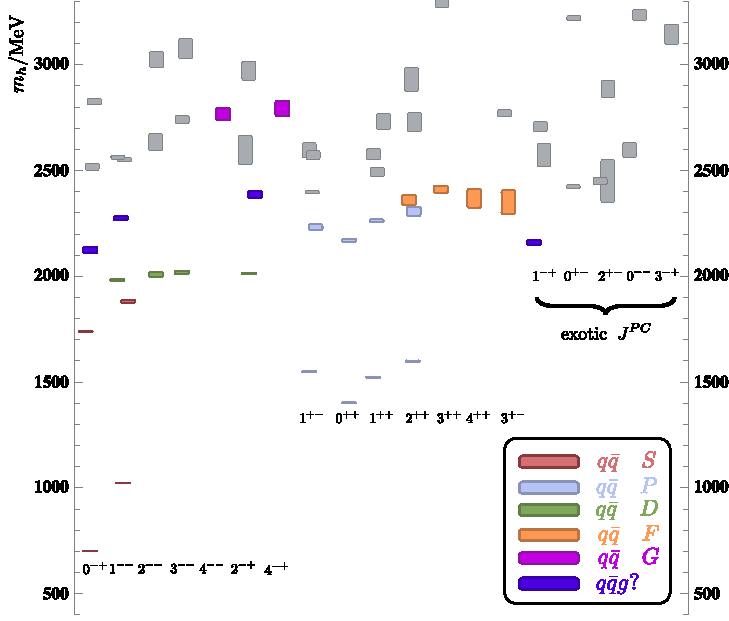
\includegraphics[width=\linewidth]{figures/LatticeSpectrum743/SpinAndWaveIdentAll.pdf}
\caption{ Here we present a lattice calculation where we have identified the spin, parity, and charge conjugation quantum numbers for a variety of states. Boxes represent energy levels extracted in our calculation, the size of the box corresponding to the uncertainty of the extracted energy. Different supermultiplet candidate states are grouped according to color. This calculation was performed in a version of QCD with three flavors of quarks all tuned to approximately the strange quark mass, further details of the lattices can be found in \secref{sec::res::calc_det}. \label{fig::MultipletIdent743Spec}}
\end{centering}
\end{figure}
\clearpage
}
%%%%%%%%%%%%%%%%%%%%%%%%%%%%%%%%%%%%%%%%%%%%%%%%%%%%%%%%%
%%%%%%%%%%%%%%%%%%%%%%%%%%%%%%%%%%%%%%%%%%%%%%%%%%%%%%%%%
%%%%%%%%%%%%%%%%%%%%%%%%%%%%%%%%%%%%%%%%%%%%%%%%%%%%%%%%%







\chapter{Radiative Transitions} \label{chap::radTranQM}

In the previous chapter we reviewed the constituent quark model and constructed the angular momentum wave functions for simple $q\bar{q}$ constructions. We found an allowed spectrum of states which could be labeled by their spin, parity, and charge conjugation quantum numbers, $J^{PC}$. We then proceeded to briefly examine a lattice spectrum and found that we could tentatively identify the spectrum as a conventional set of $q\bar{q}$ eigenstates supplemented by a spectrum of hybrid and exotic states. 

These hybrid states offer an intriguing opportunity to investigate some of the non-perturbative dynamics giving rise to the spectrum of QCD. Specifically we will concern ourselves with the calculation of vector current matrix elements which potentially allow us to probe the underlying quark current and charge distributions within hadrons. 

Here we present a non-relativistic expansion of the vector current and identify the origin of heavy quark spin flip suppression. We then proceed to introduce the multipole expansion of vector current matrix elements which effectively organizes the vector current into reduced matrix elements of irreducible spherical tensors which encode the dynamics of hadron-hadron matrix elements. The chapter concludes with an overview of some of the phenomenology associated with radiative decays. 

%%%%%%%%%%%%%%%%%%%%%%%%%%%%%%%%%%%%%%%%%%%%%%%%%%%%%%%%%
%%%%%%%%%%%%%%%%%%%%%%%%%%%%%%%%%%%%%%%%%%%%%%%%%%%%%%%%%
%%%%%%%%%%%%%%%%%%%%%%%%%%%%%%%%%%%%%%%%%%%%%%%%%%%%%%%%%

\section{Heavy Quarks and the Vector Current} \label {QM::HQ}
\subsection{The Vector Current}
In this section we expand the vector current, $\bar{\psi}\gamma^k\psi$, in the heavy quark limit. Since we will be performing a non-relativistic reduction we use the Dirac gamma matrix convention,

\begin{equation*}
\gamma^0 = \begin{pmatrix}
1 & 0 \\
0 & -1 
\end{pmatrix}
\qquad \qquad
\gamma^k = \begin{pmatrix}
0 & \sigma_k \\
-\sigma_k & 0
\end{pmatrix}.
\end{equation*}
The $\sigma_k$ are the Pauli Matrices,  
\begin{equation*}
\sigma_1 = \begin{pmatrix}0 & 1 \\ 1 & 0\end{pmatrix} \qquad \quad
\sigma_2 = \begin{pmatrix}0 & -i \\ i & 0\end{pmatrix} \qquad \quad
\sigma_3 = \begin{pmatrix}1 & 0 \\ 0 & -1\end{pmatrix}.
\end{equation*}
In this normalization the matrices satisfy the commutation relation $\left[ \sigma_i , \sigma_j \right] = 2i \epsilon_{ijk} \sigma_k $ as well as the anti-commutation relation $\{ \sigma_i , \sigma_j \} =  2\delta_{ij}$.

The quark fields, $\psi$, are represented by vectors in Dirac space which are solutions to the free Dirac equation. 
\begin{equation*}
\big[ i \gamma^\mu \partial_\mu - m_q \big] \psi= 0 
\end{equation*}
The quark field, $\psi$, can be represented in terms of ladder operators: 
\begin{equation*}
\psi(\vec{x}) = \int \frac{d^3p}{(2\pi)^3} \frac{1}{\sqrt{2E_{\vec{p}}}}\sum_{s=\pm}\left[ a^s_{\vec{p}} u^s(\vec{p}) e^{-i\vec{p}\cdot \vec{x}} + b^{s\dagger}_{\vec{p}} v^s(\vec{p}) e^{i\vec{p}\cdot \vec{x}}\right],
\end{equation*}
and the creation and annihilation operators for quarks and antiquarks obey the anti commutation rules, 
\begin{equation*}
\{a_{\vec{p}}^r , a_{\vec{q}}^{s\dagger}\} = \{b_{\vec{p}}^r , b_{\vec{q}}^{s\dagger}\} = (2\pi)^3 \delta^3(\vec{p}-\vec{q})\delta_{r,s}, 
\end{equation*}
with all other anticommutators equal to zero. 

For our purposes it will be sufficient to consider only the positive frequency solutions to the Dirac equation\footnote{We seek a non-relativistic reduction of the current operator $\bar{\psi}\gamma^k\psi$. Writing out the current we find four terms ($a^\dagger a, a^\dagger b , b^\dagger a, b^\dagger b$). Under normal ordering terms proportional to $a^\dagger b $  and $b^\dagger a$ will not contribute. The negative frequency solution ($b^\dagger b$) simply provides a copy of the positive frequency result with quarks exchanged for anti-quarks.}, they are given by\footnote{$\psi^{+}(\vec{x}) = \sum_{s=\pm}\int \frac{d^3p}{(2\pi)^3} \ \psi^{(+)}_{ \vec{p} ,s}(\vec{x})a^s_{\vec{p}}e^{-i\vec{p}\cdot\vec{x}}$ -- we are concerned with the general form of the vector current and it is sufficient to consider only a single momentum.}
\begin{equation*}
\psi^{(+)}_{ \vec{p} ,s}(\vec{x}) = \frac{1}{\sqrt{2E_{\vec{p}}}} u^s(\vec{p}) e^{-i\vec{p}\cdot\vec{x}} \qquad \qquad u^s(\vec{p}) = \sqrt{E_{\vec{p}} + m_q} \begin{bmatrix}1\\ \frac{\vec{\sigma}\cdot \vec{p}}{E_{\vec{p}} + m_q}\end{bmatrix}\chi^{(s)}.
\end{equation*}
$\chi^{(s)}$ is a two-spinor representing a spin 1/2 particle and satisfying $\chi^{(s')\dagger}\chi^{(s)} = \delta_{s's}$. Choosing to quantize along the z-axis yields
\begin{equation*}
\chi^{(\frac{1}{2})} = \begin{bmatrix}1 \\ 0 \end{bmatrix} \qquad \qquad 
\chi^{(-\frac{1}{2})} = \begin{bmatrix}0 \\ 1 \end{bmatrix}.
\end{equation*}

In quantum field theory the dual form of a quark field is given by $\bar{\psi} \equiv \psi^\dagger \gamma^0$. The extra factor of $\gamma^0$ relative to the hermitian adjoint is introduced in order to make bilinear forms well behaved under Lorentz transformations (e.g. $\bar{\psi}\psi$ is a Lorentz scalar while $\psi^\dagger \psi$ is not). Some details of the transformations of Dirac bilinears under Lorentz transformations can be found in \secref{sec::bilinearTransformations}.

Having introduced the machinery and notation we now turn to the problem at hand, namely extracting the heavy quark limit of the bilinear $\bar{\psi} \gamma^k \psi $ which, when contracted with a photon field, provides the interaction between photons and quarks in QED. Explicitly writing the structure of the current we see 
\begin{align*}
&\bar{\psi }_{ \vec{p}\,' ,s'}(\vec{x})  \gamma^k \psi_{\vec{p}, s}(\vec{x}) \\
&\quad= \frac{e^{i\vec{p}\,' \cdot \vec{x}}}{\sqrt{2E_{\vec{p}\,'}}}u(\vec{p}\,',s')^\dagger \gamma^0\gamma^k u(\vec{p},s) \frac{e^{-i\vec{p} \cdot \vec{x}}}{\sqrt{2E_{\vec{p}}}} \\
&\quad= \frac{e^{i (\vec{p}\,'-\vec{p})\cdot \vec{x}} \sqrt{E_{\vec{p}\,'} + m_q}\sqrt{E_{\vec{p}} + m_q}}{\sqrt{2E_{\vec{p}\,'}}\sqrt{2E_{\vec{p}}}}  \;\chi^{(s')\dagger} \left( \frac{\vec{\sigma}\cdot \vec{p}\,'}{E_{\vec{p}\,'} + m_q} \sigma_k +  \sigma_k\frac{\vec{\sigma}\cdot \vec{p}}{E_{\vec{p}} + m_q} \right) \chi^{(s)}.
\end{align*} 

The r.h.s. of the above equation can be further manipulated using the identity $ \left( \vec{\sigma} \cdot \vec{a} \right) \sigma_k = a_k - i \left[ \vec{a} \times \vec{\sigma} \right]_k $, one finds:
\begin{align*}
&\psibar_{\vec{p}\,' ,s'}(\vec{x})   \gamma^k \psi_{\vec{p}, s}(\vec{x}) = \\
&\quad \frac{e^{i (\vec{p}\,'-\vec{p})\cdot \vec{x}}  \sqrt{E_{\vec{p}\,'} + m_q}\sqrt{E_{\vec{p}} + m_q}}{\sqrt{2E_{\vec{p}\,'}}\sqrt{2E_{\vec{p}}}} \;\chi^{(s')\dagger} \left( \frac{ p'_k - i\left[ \vec{p}\,' \times \vec{\sigma} \right]_k}{E_{\vec{p}\,'} + m_q} +  \frac{ p_k + i\left[\vec{p} \times \vec{\sigma} \right]_k}{E_{\vec{p}} + m_q} \right) \chi^{(s)}. 
\end{align*} 
Choosing to work in the frame $|\vec{p}| = |\vec{p}\,'|$ simplifies the result considerably. We find 
\begin{equation*}
\psibar_{\vec{p}\,' ,s'}(\vec{x})  \gamma^k \psi_{\vec{p}, s}(\vec{x}) = \frac{e^{i \vec{q}\cdot\vec{x}} }{2E_{\vec{p}}} \;\chi^{(s')\dagger} \Big(  \left[ p' + p\right]_k  -i\left[\vec{q} \times \vec{\sigma} \right]_k \Big) \chi^{(s)}. 
\end{equation*} 
where $\vec{q} = \vec{p}\,' - \vec{p}$. Recalling that we are working in the limit of large quark mass we remind the reader that in this limit the momentum transfer, $\vec{q}$ is also much smaller than the momentum of the struck quark $\vec{p}$. This is akin to trying to deflect a bowling ball with a ping-pong ball. The relative difference in inertial masses mean that the impulse delivered to the bowling ball is very small relative to the momentum of the bowling ball.  

Expanding the energy for momenta small relative to the quark mass we arrive at\footnote{Working only to order $m^{-1}$ negates the need for making the simplification $|\vec{p}| = |\vec{p}\,'|$.} 
\begin{align*}
&\psibar_{\vec{p}\,' ,s'}(\vec{x})  \gamma^k \psi_{\vec{p}, s}(\vec{x}) \\
&\quad= e^{i \vec{q}\cdot \vec{x}}  \;\chi^{(s')\dagger}\left(  \frac{\left[ p' + p\right]_k}{2m_q}  -i \frac{\left[\vec{q} \times \vec{\sigma} \right]_k}{2m_q} \right) \chi^{(s)} \left( 1 - \frac{1}{2} \frac{p^2}{m_q^2} + \frac{3}{8}\frac{p^4}{m_q^4}   \right) +  \mathcal{O}(\frac{p^6}{m_q^6}). 
\end{align*}
It is sufficient for our purposes to work only to order $m^{-1}$. Exchanging the momenta for a velocity-like term ($\vec{v} = \frac{ \vec{p}\,' + \vec{p}}{2m_q}$), which has a good limit as the quark mass becomes arbitrarily large, the non-relativistic vector current is 
\begin{equation}
\mathcal{J}^k_{\mathrm{NR}}(\vec{p}\,'s',\vec{p}\,s;\vec{x})= e^{i \vec{q} \cdot \vec{x}}  \;\chi^{(s')\dagger} \left(   \vec{v}_k -i \frac{\left[\vec{q} \times \vec{\sigma} \right]_k}{2m_q} \right) \chi^{(s)}. \label{eqn::hq_vector_current_expansion}
\end{equation} 

The second term appearing between the spinors flips the spin of the quark and is the origin of \emph{heavy quark spin-flip suppression} which is the notion that matrix elements of the vector current involving quark spin flips are depleted relative to those which leave the spin wave-function untouched. For example  a $^{2S+1}L_J$ = $^3S_1$ state decaying to  $^1S_0$ should, from the viewpoint of a quark model, be suppressed by a power of the quark mass since the structure of the spin wave-function changes from triplet to singlet. 

%%%%%%%%%%%%%%%%%%%%%%%%%%%%%%%%%%%%%%%%%%%%%%%%%%%%%%%%%
%%%%%%%%%%%%%%%%%%%%%%%%%%%%%%%%%%%%%%%%%%%%%%%%%%%%%%%%%
%%%%%%%%%%%%%%%%%%%%%%%%%%%%%%%%%%%%%%%%%%%%%%%%%%%%%%%%%

\subsection{Multipole Expansion}
Having demonstrated the expansion of the vector current in the case of heavy quarks we now turn to the expansion of the result in terms of multipoles. This procedure eventually reduces to organizing the vector current into a sum over irreducible spherical tensors. The multipole elements then correspond to the reduced matrix elements of these irreducible tensors. 

As usual when considering angular momenta it is most convenient to work in a spherical basis. We choose to quantize along the z-axis. The vector current can be rewritten in terms of its angular momentum components which we label by $m$. The components are defined by

\begin{equation} 
\mathcal{J}^m_{NR}(\vec{p}\,'s',\vec{p}\,s;r)  \equiv \vec{\varepsilon}\,(\vec{q},m) \cdot \vec{\mathcal{J}}_{\mathrm{NR}}(\vec{p}\,'s',ps;r)\label{eqn::hq_vector_current_expansion_ang}
\end{equation}
where $\vec{\varepsilon}\,(\vec{q},m) $ represents a polarization vector for a spin-1 particle quantized about the z-axis. We use the basis 
\begin{gather*}
\vec{\varepsilon}\,(\vec{q} = |q| \hat{z},m=0) = \left[ 0, 0, E/m \right] \\
\vec{\varepsilon}\,(\vec{q}= |q| \hat{z},m=\pm) = \mp \frac{1}{\sqrt{2}}\left[ 1, \pm i , 0 \right].
\end{gather*}

 The plane wave appearing in the vector current (\eqnref{eqn::hq_vector_current_expansion}) can be expanded into products of Bessel functions and Legendre polynomials (Wigner D-matrices) using    
 \begin{equation*}
e^{i\vec{k}\cdot\vec{x}} = \sum_{l=0}^{l = \infty} i^l (2l+1) j_l(kx) P_l(\cos \theta) =  \sum_{l=0}^{l = \infty} i^l (2l+1) j_l(kx) D^{(l)}_{0,0}(0,\theta,0)
\end{equation*}
where we have used the fact that $P_l(\cos\beta) = D^{(l)}_{0,0}(\alpha=0,\beta,\gamma=0)$.


Rewriting \eqnref{eqn::hq_vector_current_expansion} in terms of its angular decomposition yields 
\begin{align*}
\mathcal{J}^m_{NR}(\vec{p}\,'s',\vec{p}\,s;r) &= \sum_{l=0}^{l = \infty} i^l (2l+1) j_l(qr) D^{(l)}_{0,0}(\theta) \\ 
& \qquad \quad \times \left[ \sum_k \varepsilon_k(\vec{q},m)\chi^{(s')\dagger} \left(   \vec{v}_k+ -i \frac{\left[\vec{q} \times \vec{\sigma} \right]_k}{2m_q} \right) \chi^{(s)} \right]. 
\end{align*}
In order to elucidate the transformation properties of the current it is useful to decompose the term in brackets into spherical tensors. 

Specializing our discussion to \emph{real} photons ($m =\pm$) and recalling that for a real photon the polarization is orthogonal to the momentum we can use the scalar triple product identity to rewrite the term featuring a cross-product as 
\begin{align*}
\vec{\varepsilon}(\vec{q},m) \cdot \left[ \vec{q} \times \vec{\sigma} \right] &= \vec{\sigma} \,\cdot \left[ \vec{\varepsilon}\,(\vec{q},m) \times \vec{q} \,\right]  \\
&=  is_m \vec{\sigma} \,\cdot  \vec{\varepsilon}\,(\vec{q},m) |\vec{q}\,| 
\end{align*}
where the variable $s_m$ takes the sign of the spin projection,  $s_+ = 1$ and $s_- = -1$.  So it follows that the combination $\vec{\varepsilon}(\vec{q},m) \cdot \left[ \vec{q} \times \vec{\sigma} \right] $ is nothing more than a raising or lowering operator acting in spinor-space. The vector current becomes 
\begin{equation}
\mathcal{J}^m_{NR}(\vec{p}\,'s',\vec{p}\,s;r) = \sum_{l=0}^{l = \infty} i^l (2l+1) j_l(qr) D^{(l)}_{0,0}(\theta) \left[  \vec{v}_m \delta_{s's}+ s_m\frac{|\vec{q}\,|}{2m} \chi^{(s')\dagger} \vec{\sigma}_{m}  \chi^{(s)} \right]. \label{QM::vec_curren_partial_decomp}
\end{equation}
Both terms transform like spin-1 under rotations. Upon inspection one sees that the velocity term transforms like a vector, it is negative under parity.  The magnetic dipole term, $\chi^{(s')\dagger} \vec{\sigma}_r  \chi^{(s)}$, originates from an axial vector appearing in a cross product with an ordinary vector, it too is negative under parity. 

The problem now reduces to reorganizing the current into a sum over irreducible spherical tensors. Such a tensor is defined by its transformation properties under rotations, namely a rank-$k$ spherical tensor transforms as 
\begin{equation*}
U(R)\mathcal{T}^{(k)}_m U(R)^\dagger = \sum_{m'} \mathcal{T}^{(k)}_{m'}D^{(k)}_{m'm}(R).
\end{equation*}
Where $U(R)$ is a unitary representation of the rotation, $R$, and $D^{(k)}_{m'm}(R)$ is a Wigner D-matrix. 

The angular structure of the current can then be exposed via the group theoretic projection formula (orthogonality relation)
\begin{equation*}
\int dR \; D^{(J')}_{m_1' ,m_2'}(R) D^{(J)}_{m_1 ,m_2}(R) = \frac{8\pi^2}{2J+1} \delta_{JJ'}\delta_{m_1' m_1} \delta_{m_2' m_2}
\end{equation*}
which allows us to pick out various components of arbitrary rank tensors. The integral, $\int dR$, is an integral over the group space, for example the three Euler angles. Projecting out the various irreducible spherical tensors we find the generic formula
\begin{align*}
\mathcal{T}^{(k)}_m = \frac{2J+1}{8\pi^2} \int dR \; U(R) \mathcal{J}^{m'}_{NR}(\vec{p}\,'s',\vec{p}\,s;r) U(R)^\dagger \; D^{(k)}_{m0}(R)
\end{align*}
which tells us how to access any given term in the expansion. 

Generically these current operators will appear sandwiched between states of definite angular momentum which taken with the symmetries of the current restrict the various values of $k$ that may appear. The multipole moments are then identified with the reduced matrix elements in the standard way, denoting the spin, parity, and spin projection eigenstate using $|J^{P}m\rangle$, the reduced matrix elements are given by 
\begin{equation}
\langle J'^{P'} m'  | \mathcal{T}^{(k)}_{\bar{m}} | J^P m \rangle 
= (-1)^{m+J'-k}\begin{pmatrix}J' & k & J \\ m' & \bar{m} & -m\end{pmatrix} \langle J'^{P'} || T^{(k)} || J^P\rangle  \label{QM::3J_decomp}.
\end{equation}
One conventional labeling of the reduced matrix elements is 
\begin{equation*}
\langle J'^{P'} || T^{(k)} || J^{P} \rangle = \frac{1}{2} \Big[ \left( 1 + (-1)^k\delta P \right) E_k + \left( 1 - (-1)^k\delta P \right) M_k\Big] \label{QM::multipole_convention}
\end{equation*}
where $E_k$ and $M_k$ are the electric and magnetic multipole moments and $\delta P$ is the product of the initial and final state parities. This redefinition separates electric from magnetic transitions based on the relative parity of the initial and final state -- for a given $k$ the transition is either of magnetic or electric type. 

There is in fact a phenomenological hierarchy of multipole amplitudes associated with this decomposition. Returning, for a moment, to $q\bar{q}$ angular momentum wave functions within the quark model, we recall that the allowed $J^{PC}$ quantum numbers followed from the symmetries of the $q\bar{q}$ angular momentum constructions. We first coupled the spins of the two fermions into $S=0,1$ and then added in relative orbital angular momentum to form $|L -S| \leq J \leq L+S$. Within our non-relativistic expansion of the vector current the current can either leave the spin wave function invariant or flip the spin of one of the quarks moving from $S=0$ to $S=1$ or vice versa. This may be seen by considering  \eqnref{QM::vec_curren_partial_decomp}. The term in brackets may be rewritten as 
\begin{equation}
\vec{v}_m \delta_{s's}+ s_m\frac{|\vec{q}\,|}{2m} \chi^{(s')\dagger} \vec{\sigma}_{m}  \chi^{(s)} = \vec{v}_m \delta_{s's}  -\frac{|\vec{q}|}{\sqrt{2}m}\delta_{s',s+m}.
\end{equation}
Here we explicitly see that transitions involving quark spin flips get suppressed by a power of the quark mass. Using this decomposition in conjunction with our definition of the multipole matrix elements one can show that the two terms occurring above can be identified as the origins of electric and magnetic multipole transitions respectively. 

As a simple example we can consider a vector ($^3S_1$) state radiatively decaying to a pseudoscalar ($^1S_0$). Using \eqnref{QM::3J_decomp} we see that in order for the 3-$J$ symbol to be non-zero we must have $k=1$. Since the initial and final states are both $S$-wave we see that the product of the initial and final parities is positive an by inspection of \eqnref{QM::multipole_convention} we can identify the transition to be of magnetic dipole type ($M_1$). Now inspecting the relative spin wave functions we also notice that we move from triplet to singlet, a spin flip has occurred. Thus on the basis of our non-relativistic model we expect this transition to be suppressed by the quark mass. 

The current can potentially also connect states of the same spin but different spin projections, for example consider a vector meson interacting with an external photon field via the absorption of a photon which changes the spin wave function from positive to zero spin projection ( $|\!\!\uparrow \uparrow \rangle \rightarrow |\!\!\uparrow \downarrow \rangle +  |\!\!\downarrow \uparrow \rangle$ ) -- this too should be suppressed. 

Transitions in this vein have in fact already been calculated non-perturbatively on the lattice in the charmonium sector where the quark model is expected to be rather successful owing to the heavy nature of the charm quark.  $\chi_{c_1}\rightarrow \gamma J/\psi$ and $\chi_{c_2} \rightarrow \gamma J/\psi$ were calculated using lattice QCD in \cite{Dudek:2009kk,Dudek:2006ej}. For the $\chi_c$ transitions\footnote{$\chi_{c_J} \sim \;^3P_J$} the expected hierarchy of multipoles was observed. In particular for $\chi_{c_1}\rightarrow \gamma J/\psi$ there are three transition amplitudes, one longitudinal\footnote{When considering off shell photons there is a third polarization state, the longitudinal state, corresponding to helicity zero.}, and two transverse ($E_1, M_2$); the authors found that $|\frac{M_2}{E_1}| \sim 0.1$. A similar relative scaling was found in $\chi_{c_2} \rightarrow \gamma J/\psi$, here there are five multipoles, three transverse and two longitudinal. The authors extracted $\frac{M_2}{\sqrt{E_1^2 + M_2^2 + E_3^2}} \sim 0.4$ and $\frac{E_3}{\sqrt{E_1^2 + M_2^2 + E_3^2}} \sim 0.01$.

The gradation of sizes of multipole amplitudes will be of particular interest in our analysis. We expect, on the basis of this non-relativistic expansion for heavy quarks, that all magnetic transitions for conventional $q\bar{q}$ mesons are suppressed.  One possible signal of observation of a non-conventional meson is then a large magnetic transition amplitude where the photon provides the angular momentum for an excitation of gluonic origin. In some sense we will be looking for transitions that do not fit within the expected pattern in the hopes that they may provide some insight into the gauge degrees of freedom of QCD. 

%\footnote{The term quenched refers to an approximation used in earlier calculations where the fermion determinant occurring in the probability density along which we draw configurations is set to 1 in order to reduce the computational complexity of the calculation. Such an approximation effectively removes quark loops from the calculation an may be well motivated at high quark mass where we expect the loops to scale like $m^{-1}$.} 
%%%%%%%%%%%%%%%%%%%%%%%%%%%%%%%%%%%%%%%%%%%%%%%%%%%%%%%%%
%%%%%%%%%%%%%%%%%%%%%%%%%%%%%%%%%%%%%%%%%%%%%%%%%%%%%%%%%
%%%%%%%%%%%%%%%%%%%%%%%%%%%%%%%%%%%%%%%%%%%%%%%%%%%%%%%%%


\chapter{Lattice Gauge Theory} \label{chap::lattice_gauge_thy}

%%%%%%%%%%%%%%%%%%%%%%%%%%%%%%%%%%%%%%%%%%%%%%%%%%%%%%%%%
%%%%%%%%%%%%%%%%%%%%%%%%%%%%%%%%%%%%%%%%%%%%%%%%%%%%%%%%%
%%%%%%%%%%%%%%%%%%%%%%%%%%%%%%%%%%%%%%%%%%%%%%%%%%%%%%%%%
%lattice
The properties of hadrons constructed from strongly interacting quarks and gluons should be calculable within the relevant gauge field theory, Quantum Chromodynamics (QCD). At the energy scale of hadrons, QCD does not have a small coupling constant and must be treated non-perturbatively. The tool we will use to achieve this is lattice QCD, in which the field theory is discretized on a finite grid of Euclidean space-time points, and where we can compute correlation functions as an average over a finite but large number of possible gauge-field configurations. 
%In this chapter we will explore the gauge theory, QCD, and show how one can formulate the theory onto a discrete set of space-time points, which when coupled with an analytic continuation of time, allows for the calculation of observables. 

%%%%%%%%%%%%%%%%%%%%%%%%%%%%%%%%%%%%%%%%%%%%%%%%%%%%%%%%%
%%%%%%%%%%%%%%%%%%%%%%%%%%%%%%%%%%%%%%%%%%%%%%%%%%%%%%%%%
%%%%%%%%%%%%%%%%%%%%%%%%%%%%%%%%%%%%%%%%%%%%%%%%%%%%%%%%%

\section{The Path Integral  } \label{QCD::path_integral}
The functional integral formalism underpins modern understanding of quantum field theory. It was originally introduced by Feynman in the context of quantum mechanics, later gaining widespread use in quantum field theory. Here we sketch the basics of the path integral approach used to simulate QCD.  We will work in natural units in which $\hbar = c = 1$.  

%Throughout this section we will follow the traditional \emph{physics style} mathematics in which we use words like ``function" and ``eigenstate" improperly, exchange the order of limits, and commute integrals without consideration for the deeper mathematical issues in the interest of skipping technical details that would obscure the physical understanding. 

The two most fundamental objects we will be working with are the QCD Lagrangian, $\mathcal{L}_{\mathrm{QCD}}$, and the generating functional, $\mathcal{Z}_{\mathrm{QCD}}$. The Minkowski Lagrangian is

\begin{equation}
\mathcal{L}_{\mathrm{QCD}} = \bar{\psi}\left[i \gamma_\mu \partial^\mu - m\right]\psi + g  A_\mu^a\bar{\psi}\gamma^\mu t_a\psi - \frac{1}{4}G_{\mu\nu}^aG^{\mu\nu}_a.
\end{equation}

The quark fields, denoted by $\psi^\alpha_i(x)$,  are color-spinor fields which are functions of the space-time coordinate, $x$, with a $SU(3)$ color index $i=1,2,3$ and a Dirac spinor index $\alpha=0,1,2,3$. The quark fields transform locally\footnote{Under a gauge transformation the quark field transforms as $\psi^\alpha_i(x) \rightarrow \mathcal{G}_{ij}(x)\psi^\alpha_j(x)$, where $\mathcal{G}_{ij}(x)$ is an element of $SU(3)$ representing the gauge transformation at space-time point $x$.} under $SU(3)$ color gauge rotations while the Lagrange density is a \emph{gauge invariant} scalar density. 

The gluon fields, $A_\mu^a$, transform as Lorentz vectors and have a color index $a=1-8$ corresponding to the adjoint representation of $SU(3)$ while the $t^a$ are the generators of the gauge group, one possible basis being the Gell-Mann matrices. 

The $\gamma_\mu$ are Dirac matrices and in \emph{Minkowski} space obey the anti-commutation relation $\{\gamma_\mu,\gamma_\nu\} \equiv \gamma_\mu\gamma_\nu - \gamma_\nu\gamma_\mu = 2g_{\mu\nu}$\footnote{$g_{\mu\nu}=\mathrm{diag}(+---)$}.  $G_{\mu\nu}^a$ is the field strength tensor for the chromo-magnetic and chromo-electric fields, it is defined as 
\begin{equation*}
G_{\mu\nu}^a = \partial_\mu A_\nu^a - \partial_\nu A_\mu^a - gf^{abc}A^b_\mu A^c_\nu,
\end{equation*}
where $g$ is the coupling and $f^{abc}$ are the structure constants which re-express the Lie brackets of pairs of generators as a linear combination of generators from the same set (i.e. $\left[t^a,t^b\right] = i f^{abc}t^c$).

Having introduced the Lagrangian, we may now turn to the QCD generating functional, it is defined as
\begin{equation*}
\mathcal{Z}_{\mathrm{QCD}} = \int D[\psi,\bar{\psi},A] e^{iS[\psi,\bar{\psi},A]},
\end{equation*} 
which on its own is a non-convergent oscillating integral\footnote{This integral may be defined using for example an $i\epsilon$-prescription. The functional differential, $D[\psi,\bar{\psi},A]$, stands for `integrate over all possible values the field can take at each point in space-time'. We will instead choose to regulate the integral via a Wick rotation which effectively corresponds to integrating along the imaginary direction in time.}. In this expression $S$ is the action, 
\begin{equation*}
S = \int d^4x \mathcal{L}_{\mathrm{QCD}}(x).
\end{equation*}
In order to regularize the functional integral we perform an operation called a \emph{Wick Rotation}. Formally this is an analytic continuation of time into the complex plane which can be practically achieved by taking $t=-i\tau$ for $\tau >0$. This has the advantage of replacing the oscillating weight, $e^{-iS}$, occurring in the generating functional with an exponential damping, $e^{-S}$. 

Specializing our discussion from this point forward to the \emph{Euclidean} path integral  we see the generating functional becomes 
\begin{equation}
\mathcal{Z}_{\mathrm{QCD}} = \int D[\psi,\bar{\psi},A] e^{-S[\psi,\bar{\psi},A]}. 
\end{equation} 
Working in a Euclidean space-time we now introduce the field theoretic quantities of interest, \emph{correlation functions}, which encode information about the spectrum and matrix elements we wish to extract. These correlation functions may be written in a compact manner in path integral form. Allowing, for the moment, a somewhat nebulous definition of an \emph{operator} as a collection of quark and gluon fields, the expectation of these operators may be written as
\begin{equation*}
\langle 0 | \mathcal{T}\{ \hat{\mathcal{O}}_1(t_1) \cdots \hat{\mathcal{O}}_n(t_n) \} | 0 \rangle =  \frac{1}{\mathcal{Z}_{\mathrm{QCD}}}\int D[\psi,\bar{\psi},A] e^{-S[\psi,\bar{\psi},A]} \mathcal{O}_1(t_1)\cdots \mathcal{O}_n(t_n). 
\end{equation*}
Here, and from this point forward, it is to be understood that $t$ represents a time variable that has been analytically continued via a Wick Rotation. 

We stop for a moment to point out one noteworthy property of the preceding equation, namely that on the l.h.s we have \emph{operators} which are operator valued functions of the quark and gluon fields -- on the left the quark and gluon fields are operators\footnote{By this we mean that we could reexpress the quark and gluon fields as creation and annihilation operators for one-particle states.}. This is to be contrasted with the r.h.s. where the quark and gluon fields are just numbers which should be integrated over.  

Integrating over all possible field configurations should be expected to be an arduous task, in fact we do not yet know how to compute  functional integrals analytically except for a few simple systems\footnote{For example the harmonic oscillator in non-relativistic quantum mechanics}. One technique, which allows the integral to be estimated numerically, involves discretizing spacetime onto a mesh of points. This process, of discretizing the path integral, essentially defines a scheme in which we can calculate correlation functions. We will now proceed to sketch the basics of the numerical approach to estimating the path integral of lattice QCD.  

Working in a discrete space-time it is natural to label the nodes of the lattice by a vector of integers, $\vec{n} = [n_x , n_y , n_z , n_t]$. Using $a$ to denote the lattice spacing, the allowed space-time coordinates are $\vec{x}_{\vec{n}} = a\;\vec{n}$. Here we will specialize to a case where the length of the box is the same in all directions, $L_{x}= L_{y} = L_z = L_t = N a = L$, where we have imagined that we have divided each direction into $N$ segments\footnote{Later in the text we will consider QCD on an anisotropic lattice where the discretization along the temporal direction is finer than along the spatial directions.}. 

The quark fields, $\psi^\alpha_i(x)$, reside on the nodes of the lattice. They are chosen to obey periodic boundary conditions in the spatial direction,  $\psi^\alpha_i(x) = \psi^\alpha_i(x + L)$, and anti-periodic boundary conditions in time\footnote{One could in principle choose alternate boundary conditions for the spatial directions -- periodic B.C. will be useful in our calculation as they naturally allow for quantization of momentum in units of $2\pi/L$. The anti-periodic boundary conditions in time are a consequence of putting fermions on a toroid, the sign must be introduced to make the density matrix positive definite.}. 

In the continuum theory the gluon fields $A^a_\mu$ appear in the \emph{parallel transporters} 
\begin{equation*}
U(x,y) \equiv \mathcal{P}\{e^{ig \int_x^y dz_\mu A^c_\mu(z) t^c }\}
\end{equation*} 
which tell us how to accumulate color phase as we move through space. Here the symbol $\mathcal{P}$ denotes a path ordering and means to compute the exponentiated integral along some specific path from $x$ to $y$. When we discretize the theory the parallel transporters must be anchored at the nodes of the lattice, we call the resulting transporters which take us from one node to its neighbor \emph{gauge links}, they are elements of $SU(3)$ and are defined as: 
\begin{equation*}
U_\mu(x) \equiv U(x,x+\hat{\mu}) =  e^{ig a A^c_\mu(x) t^c }. 
\end{equation*} 
Where $a$ is the lattice spacing along the $\mu$ direction\footnote{Note the variable change, when talking about gauge fields in the context of a lattice discretization we exchange the field variable, $A^c_\mu(x)$, for the link variable $U_\mu(x)$ which is the parallel transporter taking us from site $x$ to site $x+a\hat{\mu}$ along the \emph{straight line path}, not for example a path that has the shape of a staple, which is an important distinction in non-abelian theories.}. 

In \figref{fig::QCD_1p1_lattice_fields} we show a toy representation of the discretization of QCD in $1+1$ dimensions. The fermion fields ``live" on the lattice sites while the gluons are contained in the gauge links that connect neighboring sites. The operators $\mathcal{O}$,  defined in more detail in \secref{sec::Spec:ops}, are constructed out of gauge invariant combinations of the quark fields and gauge links. 

\afterpage{
\begin{figure}[htbp]
\centering
\includegraphics[width=0.8\linewidth]{figures/lattice_toroid_fields/lattice_toroid_fields.pdf}
\caption{ A $1+1$ dimensional toroid. When we discretize QCD onto a lattice the quark fields $\psi$ sit on the nodes of the lattice while the gluon fields live along the gauge links in the matrices $U$ which are elements of $SU(3)$. \label{fig::QCD_1p1_lattice_fields}}
\end{figure}
\clearpage
}

The discretization of the underlying field theory onto a lattice provides us a systematically improvable framework in which we can non-perturbatively evaluate correlation functions in the strongly coupled regime of QCD.



%%%%%%%%%%%%%%%%%%%%%%%%%%%%%%%%%%%%%%%%%%%%%%%%%%%%%%%%%
%%%%%%%%%%%%%%%%%%%%%%%%%%%%%%%%%%%%%%%%%%%%%%%%%%%%%%%%%
%%%%%%%%%%%%%%%%%%%%%%%%%%%%%%%%%%%%%%%%%%%%%%%%%%%%%%%%%

\section{Fermions in the Path Integral} \label{QCD::path_integral}

Having introduced the lattice discretization of the Euclidean path integral we now turn to an overview of methods which enable us to numerically estimate correlation functions. We look first to the fermion content of the path integral. Fermions anti-commute. In the language of operators this condition is imposed on the creation/annihilation field \emph{operators}. However, as mentioned previously, within the path integral formulation the fermions are replaced by \emph{numbers} which should be integrated over. In order to build in the anti-commutation under the path integral we represent the fermions by \emph{Grassman} numbers -- anti-commuting complex numbers.  A more detailed discussion of fermions and Grassman algebra can be found \appref{app::grassman}

The main result  is 
\begin{equation}
\label{eqn:fm_det}
\int d\eta d\bar{\xi}e^{\eta^TM\xi}  = \mathrm{det}(M),
\end{equation}
where $\eta$ and $\xi$ are vectors of Grassman numbers. 
 
Armed with this knowledge of Grassman integration, \eqnref{eqn:fm_det}, we now look to how we can use this formula to analytically integrate out the fermionic fields from the path integral. Recalling that we may specify any node on our lattice by a vector of integers, $\vec{n} = [n_x , n_y , n_z , n_t]$, and defining $\psi_n = \psi(a\vec{n})$, we may proceed to write the action in discretized form as 
\begin{equation*}
S[\psi,\bar{\psi},U] = S_{\mathrm{gauge}}[U]  + \sum_{n_1,n_2} \bar{\psi}_{n_1} M_{n_1,n_2}[U] \psi_{n_2} 
\end{equation*}
Where $M_{n_1,n_2}[U]$ represents the lattice discretization of the piece of the continuum Euclidean action appearing between the quark fields, $\left( \slashed{D} - m \right)$, $U$\footnote{$U$, the gauge field corresponds to a link variable. It is an element of $SU(3)$. There is a matrix, describing the gauge field, at each link on the lattice.} is the gauge field\footnote{The matrix, $M_{n_1,n_2}[U]$, contains dependence on the gauge field through the gauge covariant derivative appearing in the Lagrange density.}, and $S_\mathrm{gauge}[U]$ represents a lattice discretization of the gauge portion of the Lagrangian. The generating functional of the discretized Path Integral may be written as 
\begin{equation*}
\mathcal{Z}_{\mathrm{QCD}} = \int D[\psi,\bar{\psi},U] e^{-\bar{\psi}M[U]\psi \; - S_{\mathrm{gauge}}[U]}.
\end{equation*} 
Now using the integration formula for Grassman numbers (\eqnref{eqn:fm_det}) we see the fermion fields may be analytically integrated yielding 
\begin{equation*}
\mathcal{Z}_{\mathrm{QCD}} = \int D[U] e^{- S_{\mathrm{gauge}}[U]} \,\mathrm{det}(M[U]).
\end{equation*} 
This is an extremely powerful realization -- we do not need to represent \emph{anti-commuting complex numbers} on a computer. Further the preceding equation can be estimated via standard Markov-Chain Monte Carlo methods. 

%%%%%%%%%%%%%%%%%%%%%%%%%%%%%%%%%%%%%%%%%%%%%%%%%%%%%%%%%
%%%%%%%%%%%%%%%%%%%%%%%%%%%%%%%%%%%%%%%%%%%%%%%%%%%%%%%%%
%%%%%%%%%%%%%%%%%%%%%%%%%%%%%%%%%%%%%%%%%%%%%%%%%%%%%%%%% 
 
\subsection{Correlation Functions}

As mentioned previously, the fundamental theoretical objects of interest are correlation functions. For now it is useful to consider operators composed entirely of gauge links, we will lift this restriction after we have introduced the essential details related to the numeric estimation of correlation functions. Denoting our operator, composed only out of gauge links, as $\mathcal{O}_G$, such a correlation function takes the form
\begin{equation*}
\langle 0 | \hat{\mathcal{O}}_G  | 0 \rangle =  \frac{1}{\mathcal{Z}_{\mathrm{QCD}}}\int D[U] e^{-S_{\mathrm{gauge}}[U]} \,\mathrm{det}(M[U]) \,\mathcal{O}_G[U]. 
\end{equation*}

The simplest way one could estimate this correlation function is by drawing gauge configurations, at random, and then averaging over a finite but large number of configurations. For a lattice which contains $N$ sites along each direction there are $4N^4$ gauge links. Each link variable can be specified by eight real numbers\footnote{There are 8 generators of $SU(3)$, any element of the group can be written as $e^{i\theta_a t_a}$ where $\theta_a$ is a real number and $t_a$ is a generator. There is an implied summation on $a$.}, thus the parameter space of such a simulation is $32N^4$. Modern lattices contain roughly twenty nodes along any given direction; as a simple baseline we can consider a parameter space consisting of $512\times 10^4$ real numbers in the interval $[0,2\pi]$ -- one may expect that such a naive approach to estimating the correlation function would have poor convergence properties. 

Fortunately we can do much better. We do this by drawing the gauge configurations according to the probability density, 
\begin{equation}\label{eqn::MC_prob_dens}
P(U) = \frac{1}{\mathcal{Z}_{\mathrm{QCD}}}e^{-S_{\mathrm{gauge}}[U]} \,\mathrm{det}(M[U]).
\end{equation}
Integration methods of this form, drawing sample points according to some probability distribution, fall under the general class of algorithms called Markov Chain Monte Carlo methods\footnote{The Metropolis-Hastings algorithm is one such algorithm seen commonly in the context of numeric integration.}. 

Drawing from such a probability density also admits a classic interpretation of the integration path. Consider for a moment the principle of stationary action from Classical Mechanics. Minimization of the action corresponds roughly to a gauge field of maximum probability. Thus in an intuitive sense we can consider this formulation as sampling the Path Integral near the classical equations of motion. Those field configurations which minimize the action are exponentially preferred relative to those which are far from the classical solution\footnote{More correctly the probability is also proportional to $\det(M[U])$. The `action' in this case is then $e^{-S_G[U] + \ln(\det(M[U]))}$.}. 

By drawing a finite but large set of gauge configurations, $\{U_i\}$, according to the probability density in \eqnref{eqn::MC_prob_dens}, we can estimate the expectation value\footnote{This formulation also provides us with an estimate of the variance of the distribution.} as 
\begin{equation*}
\langle 0 | \hat{\mathcal{O}}_G  | 0 \rangle = \frac{1}{N} \sum_{\{U_i\}} \mathcal{O}_G[U_i].
\end{equation*}
More generally we will also be interested in computing correlation functions involving fermion fields. The numeric estimation of such correlation functions proceeds in the same manner and where the fermion fields are contracted together, the combination $\psi \bar{\psi}$ is replaced by the propagator, $M^{-1}[U]$. 
%Further details about Wick contractions and the evaluation of correlation functions featuring fermion fields can be found in \fcite{APPENDIX}.  

%%%%%%%%%%%%%%%%%%%%%%%%%%%%%%%%%%%%%%%%%%%%%%%%%%%%%%%%%
%%%%%%%%%%%%%%%%%%%%%%%%%%%%%%%%%%%%%%%%%%%%%%%%%%%%%%%%%
%%%%%%%%%%%%%%%%%%%%%%%%%%%%%%%%%%%%%%%%%%%%%%%%%%%%%%%%% 
 
\subsection{Symmetries and Intuition}

Having introduced the general technology used to sample correlation functions we now aim to build some intuition for the effect the lattice discretization has on our calculation. In particular we focus on the loss of rotational symmetry. When we consider QCD on a grid we do not have the ability to rotate by any infinitesimal angle as we do in the continuum. Rather, we can only perform rotations and reflections which leave the grid invariant. This means that the Hamiltonian, and thus the eigenstates, of our lattice discretized theory have a different symmetry group than their infinite volume continuum counterparts\footnote{Another way of saying this is that the operator which rotates by an infinitesimal angle does not commute with the lattice discretized Hamiltonian. The traditional set of quantum numbers must be replaced with a set that are good under cubic symmetry.}. 

\afterpage{
\begin{figure}[htbp]
\centering
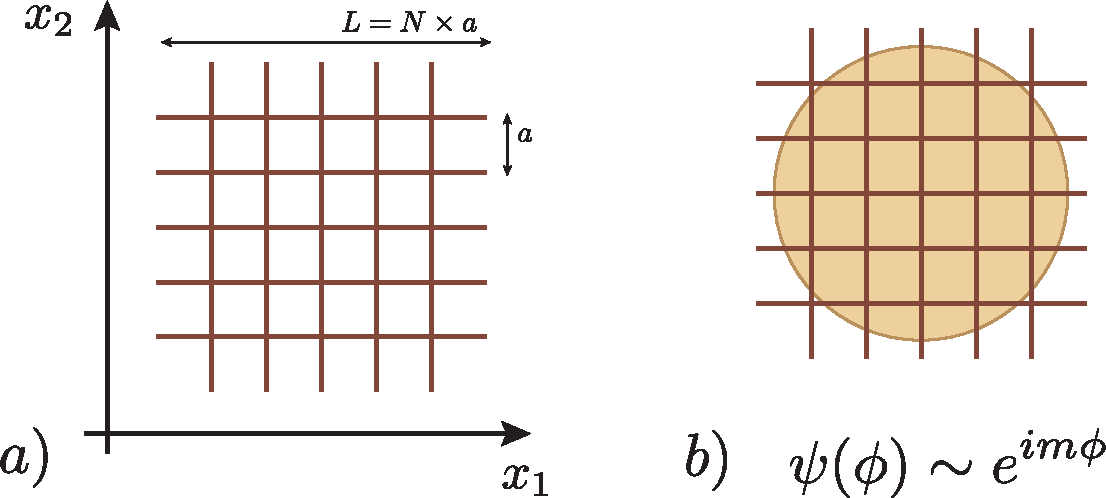
\includegraphics[width=0.7\linewidth]{figures/2DLattice/2dLatticeWavefuncs.pdf}
\caption{ A two dimensional lattice discretization. \label{fig::2DlatticeWavefuncs}}
\end{figure}
\clearpage
}

For example, if we think about a square discretization of a two dimensional theory, \figref{fig::2DlatticeWavefuncs}, we immediately realize that the square is only invariant under rotations by $\pi/2$. In a simple sense we have lost the ability to perform infinitesimal rotations which in turn mixes the angular momentum eigenstates.  For example, considering only rotations by $\pi/2$ we lose the ability to distinguish $m=0$ angular wave functions from $m=4$. 
 
This feature, reduced symmetry arising from the discretization, will reappear when we consider spectroscopy and matrix elements. We will find that particles transforming like spin-$J$ in the continuum are instead labeled by the irreducible representations of the symmetry group of the cube, multiple values of $J$ being present in any one irreducible representation. 























































\chapter{Spectroscopy on the lattice} \label{chap::Spectroscopy}

Extraction of the spectrum begins with the calculation of Euclidean two-point functions which encode the spectrum of eigenstates of lattice QCD. The functions of interest appear as matrix elements between creation and annihilation operators separated by some Euclidean distance in time. We will see that such a two-point function has a spectral representation whose time dependence is governed by the set of eigenstates of the finite volume, lattice discretized Hamiltonian, $\mathbf{H}$.  Here we present the essential details of correlator construction, a variational based analysis method which allows access to the lowest lying hadronic eigenstates, and the results from a spectroscopic calculation. 

%%%%%%%%%%%%%%%%%%%%%%%%%%%%%%%%%%%%%%%%%%%%%%%%%%%%%%%%%
%%%%%%%%%%%%%%%%%%%%%%%%%%%%%%%%%%%%%%%%%%%%%%%%%%%%%%%%%
%%%%%%%%%%%%%%%%%%%%%%%%%%%%%%%%%%%%%%%%%%%%%%%%%%%%%%%%%

\section{Correlation Functions} \label{sec::Spec:corrFunc}

Determination of the excited spectrum of QCD proceeds from the calculation of correlation functions between a \emph{basis} of creation and annihilation operators, $\{\mathcal{O}_i^\dagger\}$, separated by a distance $t$ in Euclidean time. Such a correlation function takes the form 
\begin{equation*}
C_{ij}(t) = \langle 0 | \mathcal{O}_i(t) \mathcal{O}_j^\dagger(0) | 0 \rangle 
\end{equation*}
where $|0\rangle$ denotes the vacuum. By inserting a complete set of states of the lattice discretized Hamiltonian, $\mathbf{H} | \estate{n} \rangle = E_{\estate{n}} | \estate{n} \rangle$, and time evolving the annihilation operator back to the origin, $\mathcal{O}_i(t) = e^{\mathbf{H}t} \mathcal{O}_i(0) e^{-\mathbf{H}t}$, we can decompose the correlation function into its spectral representation \footnote{In a finite volume the spectrum is discrete rather than continuous owing to the quantization of momentum ( $\mathbb{1} = \sum_{\estate{n}} \frac{1}{2E_{\estate{n}}}  | \estate{n} \rangle \langle \estate{n} |$ ). Some details of momentum conservation in a finite volume are presented in \appref{app::two-point}. } .
\begin{equation*}
C_{ij}(t) = \sum_{\estate{n}} \frac{1}{2E_{\estate{n}}} \langle 0 | \mathcal{O}_i(0) | \estate{n} \rangle \langle \estate{n} | \mathcal{O}_j^\dagger(0) | 0 \rangle e^{-E_{\estate{n}}t}
\end{equation*}

The index $\estate{n}$ runs over particle species, angular momentum, and momentum. It is worth noting that formally \emph{all} strongly interacting eigenstates, including for example the nucleus of Carbon-12, are contained in this sum. We will specialize to the case of the lowest few mesonic excitations. 

By constructing operators with good quantum numbers (e.g. total angular momentum, parity, and charge conjugation quantum numbers) we can filter the sum into excitations within a given channel. This is to say that the vacuum operator state overlaps, $ \langle \estate{n} | \mathcal{O}^\dagger(0) | 0 \rangle $, will only be non-zero if the operator $\mathcal{O}$ has the same quantum numbers as the state $\estate{n}$. 

Operators appearing in the two-point functions we consider are constructed to be gauge invariant combinations of the fundamental quark and gluon fields (gauge links).  The generic form of the operators we will use is
\begin{equation*}
\mathcal{O}_i^\dagger(t) = \sum_{\vec{x}, \vec{y} } \psibar_{\vec{x}}(t)\cdot  \mathbf{\Gamma}^i_{\vec{x} \vec{y}}(t) \cdot \psi_{\vec{y}}(t)
\end{equation*}
where $\mathbf{\Gamma}$ acts in the suppressed color and spin spaces as well as coordinate space\footnote{$\mathbf{\Gamma}$ also includes momentum projection. Later, in our three-point function analysis, we will require operators projected to be at rest as well as those projected into definite momentum.}. A two point function between two such operators may be re-expressed in terms of Wick contractions and evaluated numerically. 
\begin{align*}
 \langle 0 | \mathcal{O}_i(t) \mathcal{O}_j^\dagger(0) | 0 \rangle &= \langle 0 |\psibar_{\vec{x}}(t)\mathbf{\Gamma}^i_{\vec{x} \vec{y}}(t) \psi_{\vec{y}}(t)  \cdot \psibar_{\vec{w}}(0)\mathbf{\Gamma}^j_{\vec{w} \vec{z}}(0) \psi_{\vec{z}}(0)  | 0 \rangle \\
 &= - \trace{M^{-1}_{\vec{z}\vec{x}}(0,t)\mathbf{\Gamma}^i_{\vec{x} \vec{y}}(t)M^{-1}_{\vec{y}\vec{w}}(t,0) \mathbf{\Gamma}^j_{\vec{w} \vec{z}}(0)} \\
 & \quad\; + \trace{M^{-1}_{\vec{y}\vec{x}}(t,t) \mathbf{\Gamma}^i_{\vec{x} \vec{y}}(t)} \; \trace{M^{-1}_{\vec{z}\vec{w}}(0,0)\mathbf{\Gamma}^j_{\vec{w} \vec{z}}(0)}
\end{align*}
Here the traces are over color and spin, there are implied sums on the spatial indices. The second term involving a product of two traces is referred to as a \emph{disconnected} diagram and does not feature in the isovector correlation functions to which we specialize. 

The correlation functions are evaluated over the set of gauge configurations. We will see later in this chapter that constructing a matrix of such two point functions and inspecting the time dependence allows for robust extraction of the spectrum. The actual method we use, the variational method, becomes more powerful as one increases the redundancy of operators in a given channel of quantum numbers and, as such, we are well served by techniques that allow for both the efficient construction of a basis of operators\footnote{Details of operator construction appear in the subsequent section.} and subsequent numerical evaluation of correlation functions. Motivated by the need for a large basis in conjunction with the infrastructure to efficiently evaluate two-point functions we now turn to some of the more technical details regarding operator construction before transitioning to spectroscopic methods and results.
%Correlation functions are evaluated over the set of gauge configurations. By building up a matrix of such two point functions from we can extract spectral information via inspection of the time dependence of the matrix of correlators. Having reviewed the general mode of calculation we now turn to the details of the operator construction, smearing algorithms, and the variational calculation used in our analysis. 

%%%%%%%%%%%%%%%%%%%%%%%%%%%%%%%%%%%%%%%%%%%%%%%%%%%%%%%%%
%%%%%%%%%%%%%%%%%%%%%%%%%%%%%%%%%%%%%%%%%%%%%%%%%%%%%%%%%
%%%%%%%%%%%%%%%%%%%%%%%%%%%%%%%%%%%%%%%%%%%%%%%%%%%%%%%%%

\section{Operator Construction} \label{sec::Spec:ops}
We will only be considering the lightest few mesonic excitations and as such it is judicious to construct operators which overlap predominantly onto the low modes of the theory with reduced overlap onto higher lying excitations which are not of interest. One well-known way of improving operator overlap onto the lightest set of hadrons is `smearing' \cite{Allton:1993wc}. The thrust of these methods is to construct a new set of fields, as a combination of the fields appearing in the Lagrangian, which will be used in the operator construction. 

%\footnote{The gauge field smearing used in this analysis is non-linear while the quark field smearing is linear.}

A good smearing algorithm should be gauge covariant; we do not want to change the transformation properties of the quark fields under color gauge rotations. We would also like to preserve the properties of the quark fields under parity, charge conjugation, and rotation. The smearing function we wish to use should then preserve as many symmetries as possible while removing the presence of short range modes, which do not contribute to the long range physics we are interested in. 

Historically the method of choice is Jacobi smearing \cite{Allton:1993wc}. This method is one of several based on use of the lattice Laplacian as a smearing function. One representation   of the Laplacian is
\begin{equation*}
-\nabla^2_{\vec{x}\vec{y}}(t) = 6 \delta_{\vec{x}\vec{y}} - \sum_{j=1}^3 \left[ U_j(\vec{x},t)\delta_{\vec{x}+\hat{j},\vec{y}} + U^\dagger_j(\vec{x}-\hat{j},t)\delta_{\vec{x}-\hat{j},\vec{y}}\right]
\end{equation*}
where $U$ represents a gauge field which may be itself be constructed from a covariant gauge field smearing algorithm \footnote{Since we are working on a grid with finite spacing introduction of a derivative introduces discretization error, relative to the continuum value, which is polynomial in $a$ the lattice spacing. Various formulations of the Laplacian, based on different finite difference derivatives (e.g. forward, backward, central), will introduce different discretization effects. }. The smearing function (operator) is defined as 
\begin{equation*}
S_{\sigma,n_\sigma}(t) = \left( 1 + \frac{\sigma \nabla^2(t)}{n_\sigma}\right)^{n_\sigma} 
\end{equation*}
where the parameters $\sigma$ and $n_\sigma$ are tunable and can be used to optimize overlap onto the states of interest. It should be understood that the smearing function $S_{\sigma,n_\sigma}(t)$ has suppressed color and space indices, it is a polynomial function of the gauge covariant Laplacian, in discretized space-time the operator becomes a matrix with color and $x$-space (3-space) indices. 

When considering the effect of smearing on quark fields it is helpful  to expose the previously suppressed color and space indices of the smearing operator
\begin{equation*}
\left[S_{\sigma,n_\sigma}(t)\right]_{\vec{x}\vec{y}}^{ij} = \left[ \left( 1 + \frac{\sigma \nabla^2(t)}{n_\sigma}\right)^{n_\sigma} \right]_{\vec{x}\vec{y}}^{ij}.
\end{equation*}
The smeared quark fields are defined as 
\begin{equation*}
\tilde{\psi}_{\vec{x}}^i(t) = \sum_{\vec{y},j} \left[S_{\sigma,n_\sigma}(t)\right]_{\vec{x}\vec{y}}^{ij} \psi_{\vec{y}}^j(t)
\end{equation*}
and can be shown to be a weighted average of the quark fields amongst neighboring sites connected by parallel transporters to ensure the proper transformation under color gauge rotations.

It is helpful to consider the limit of large $n_\sigma$ (i.e. many applications of the smearing operation). In this limit the smearing function becomes $e^{\sigma \nabla^2}$ and $\sigma$ can be thought of as a smearing width. This function exponentially damps out the higher lying eigenmodes of the Laplace operator whilst retaining the lowest modes which are of interest\footnote{Recall for the $k$'th eigenvector, $\xi^{(k)}$, the Helmholtz equation is $\nabla^2\xi^{(k)} = - \lambda_k \xi^{(k)}$. Thus $e^{\sigma \nabla^2}$ damps the projection along $k$'th eigenvector with weight $e^{-\sigma \lambda_k}$. If we consider the free field case then this smearing algorithm becomes a projection onto plane waves, $\xi^{(k)} = e^{i\vec{k}\cdot \vec{x}}$ and $\lambda_k = \vec{k}^2$.  }. Indeed in the non-interacting limit the eigenfunctions of the Laplacian are plane waves, damping out the higher modes can be intuitively understood introducing a soft momentum damping on the quark fields which should not be relevant to the spectrum of low lying hadrons. 



%%%%%%%%%%%%%%%%%%%%%%%%%%%%%%%%%%%%%%%%%%%%%%%%%%%%%%%%%
%%%%%%%%%%%%%%%%%%%%%%%%%%%%%%%%%%%%%%%%%%%%%%%%%%%%%%%%%
%%%%%%%%%%%%%%%%%%%%%%%%%%%%%%%%%%%%%%%%%%%%%%%%%%%%%%%%%

\subsection{Distillation Smearing} \label{sec::Spec:ops:Distsmear}

A more modern incarnation of Laplacian based smearing, which we choose to use, is called \emph{Distillation} \cite{Peardon:2009gh}. Distillation can be thought of as a choice of quark fields to use in our operator construction. In this formulation the smearing operator is written as an outer product of some number of vectors in position and color-space. One then exploits the outer product nature of the smearing operator to factorize correlation functions into products of matrices in the distillation space. Our implementation chooses to make use of the eigenvectors of the gauge covariant Laplacian as the smearing basis. 

% It relies on the previously mention observation that as we increase the number of smearing iterations, $n_\sigma$, the resulting smearing function approaches $e^{\sigma \nabla^2}$ which damps projections against the $k$'th eigenvector as $e^{-\sigma \lambda_k}$.
 
%  The magic of distillation is the realization that instead of exponentially damping the high lying eigenmodes we can choose to simply ignore them. This is a strong statement but may be tempered by the realization that we were free all along to choose how to write down our basis of operators. 

The algorithm proceeds as follows: 
\begin{enumerate}
\item Let $V_{D}$ be the vector space of the gauge covariant three dimensional Laplacian, it is rank $N^3\times N_c$ where $N$ is the integer length of the box and $N_c = 3$,  the number of colors.  
\item Define the distillation operator, $\Box$, on timeslice $t$ as the product of an $V_D\times N_D$ matrix, $\Xi$, and its hermitian conjugate. $N_D$ is the rank of the smearing operator and is chosen to be small $N_D << V_D$. 
\begin{equation*}
\Box(t) = \Xi(t) \Xi^\dagger(t)
\end{equation*}
\item Choose the $k$'th column of $\Xi(t)$ to be the $k$'th eigenvector of $\nabla^2$, $\xi^{(k)}$, on timeslice $t$ where the eigenvectors have been ordered by eigenvalue\footnote{In principle one can choose an alternate basis of vectors as well as include some $k$ dependent function which assigns relative weights to the vectors.}. 
\begin{equation*}
\Box(t) = \Xi(t) \Xi^\dagger(t) \quad \Longrightarrow \quad \Box_{\vec{x}\vec{y}}(t) = \sum_{k=1}^N \xi_{\vec{x}}^{(k)}(t)  \xi_{\vec{y}}^{(k)^\dagger}(t) 
\end{equation*}
\item Define the distillation smeared quark fields as
\begin{equation*}
\tilde{\psi}_{\vec{x}}(t) = \sum_{\vec{y}} \Box_{\vec{x}\vec{y}}(t) \psi_{\vec{y}}(t)
\end{equation*}
\end{enumerate}

Such a smearing operator has numerous advantages, namely, the distillation operator is scalar under rotations, covariant under gauge rotations, and is parity and charge conjugation invariant.  The operator is also idempotent, $\Box^2 = \Box$, and has the property that when we increase the number of distillation operators to be the dimension of the space $V_D$ the distillation operator becomes the identity operator and the quark fields are unsmeared. 

The biggest advantage of distillation becomes evident when we consider constructing meson operators out of distillation smeared quark fields. Such an operator may be written as 
\begin{equation*}
\mathcal{O}_i(t) =  \psibar_{\vec{x}}(t)  \Box_{\vec{x}\vec{y}}(t)  \cdot  \mathbf{\Gamma}^i_{\vec{y} \vec{z}}(t)  \cdot   \Box_{\vec{z}\vec{w}}(t) \psi_{\vec{w}}(t).
\end{equation*}
Here repeated indices, as well as the suppressed color and spin indices, are summed over.  We can write a two point function composed of two such distillation smeared operators in shorthand notation (suppressing all indices) as
\begin{align*}
C_{ij}(t) = \langle 0 | \mathcal{O}_i(t) \mathcal{O}_j^\dagger(0) | 0 \rangle &= \langle 0 |\psibar_t \Box_t\mathbf{\Gamma}_t^i \Box_t \psi_t  \cdot \psibar_0 \Box_0\mathbf{\Gamma}_0^j \Box_0\psi_0  | 0 \rangle. 
\end{align*}
 After evaluating the quark field portion of the path integral the connected portion of the two point function is 
\begin{align*}
 C_{ij}(t) = -\trace{\Box_0 M^{-1}_{0t} \Box_t \Gamma^i_t \Box_t M^{-1}_{t0} \Box_0 \Gamma^j_0}.
\end{align*}
Now exposing the outer product nature of the smearing operator we see the true ingenuity of distillation smearing, namely a factorization of the correlation function into a trace over the product of a set of $N_D\times N_D$ matrices where $N_D$ is the rank of the distillation operator. Explicitly,
\begin{align*}
 C_{ij}(t) &= - \trace{\xi^{(p)}_0 \xi^{(p)\dagger}_0 M^{-1}_{0t} \xi^{(q)}_t \xi^{(q)\dagger}_t \Gamma^i_t \xi^{(r)}_t \xi^{(r)\dagger}_t  M^{-1}_{t0} \xi^{(s)}_0 \xi^{(s)\dagger}_0 \Gamma^j_0} \\
 &= -\trace{  \left[ \xi^{(p)\dagger}_0 M^{-1}_{0t} \xi^{(q)}_t  \right] \cdot \left[  \xi^{(q)\dagger}_t \Gamma^i_t \xi^{(r)}_t  \right] \cdot \left[ \xi^{(r)\dagger}_t  M^{-1}_{t0} \xi^{(s)}_0 \right] \cdot \left[ \xi^{(s)\dagger}_0 \Gamma^j_0 \xi^{(p)}_0\right] } \\
 &= - \trace{ \tau_{pq}(0,t) \cdot \Phi^i_{qr}(t) \cdot \tau_{rs}(t,0)\cdot \Phi^j_{sp}(0)},
\end{align*}
where \footnote{Here we have used the cyclic property of the trace ($\trace{ABC} = \trace{BCA}$) to ``slide'' $\xi^{(p)}_0$ around the trace.}
\begin{equation*}
\tau_{pq}(0,t) = \xi^{(p)\dagger}_0 M^{-1}_{0t} \xi^{(q)}_t \qquad \qquad \Phi^i_{qr}(t) =   \xi^{(q)\dagger}_t \Gamma^i_t \xi^{(r)}_t.
\end{equation*}

The \emph{perambulators}, $\tau_{pq}(0,t)$, describe quark propagation while the $\Phi$ encode operator construction. Of particular note is the fact that the choice of source and sink operators $\Phi$ is completely independent of the computation of the perambulators\footnote{This is not the case in traditional smearing algorithms. Older algorithms make use of `point-to-all' propagation which requires knowledge of the source or sink prior to computation of the quark propagators.}. Indeed in practice one precomputes and stores the $\tau$ and $\Phi$, this allows for the efficient calculation of a large number of correlation functions \emph{a posteriori}. A similar factorization occurs for the disconnected correlation functions, those involving the product of two or more traces, arising in isoscalar calculations. 

The essential ingredients, needed to construct our implementation of the distillation operator, are the first few eigenvectors themselves and the object $M^{-1}\xi^{(k)}$\footnote{In practice these vectors can be efficiently extracted using conjugate gradient algorithms to solve the system $Ax=b$ where $A=M$, $b=\xi^{(k)}$, and $x$ is the aptly named solution vector we desire, $M^{-1}\xi^{(k)}$.}. We again stress the value of factorization of the correlation function. In practice the rank of the distillation operator is an $\mathcal{O}(100)$ number which should be compared to the size of the full space propagator, $M^{-1}$, a matrix of rank $\mathcal{O}(10^7)$ even in modest calculations. In practice we actually only have access to $M$, computing the unsmeared correlation function would require the inversion of this entire space of this matrix. Conversely distillation only requires $\mathcal{O}(100)$ inversions. 
%%%%%%%%%%%%%%%%%%%%%%%%%%%%%%%%%%%%%%%%%%%%%%%%%%%%%%%%%
%%%%%%%%%%%%%%%%%%%%%%%%%%%%%%%%%%%%%%%%%%%%%%%%%%%%%%%%%
%%%%%%%%%%%%%%%%%%%%%%%%%%%%%%%%%%%%%%%%%%%%%%%%%%%%%%%%%

\subsection{Meson Interpolators} \label{sec::Spec:ops:MesOps}

Having reviewed the smearing algorithms and exposed the factorization of correlation functions we are now ready to turn to the construction of the operators appearing in these functions. In general the method we use for spectroscopic analysis, the variational method, makes use of a redundancy of operators within any channel of quantum numbers, the robustness of our variational solution being tied to the size and efficacy of our basis of interpolators. 

We will proceed by first considering the simplest set of operators we can construct, local fermion bilinear operators. That is, operators of generic structure $\psibar \Gamma \psi$ where $\Gamma$ is one of the sixteen Dirac matrices (e.g. $\gamma_\mu$, $\gamma_5\gamma_\mu$, $\sigma_{\mu\nu}$).  In distillation the quark fields, $\psi$, will be replaced by the smeared fields $\tilde{\psi}$, but this does not change the nature of the operator under rotations and thus the quantum numbers will be the same. We reproduce a known result, namely that the simplest local bilinears are somewhat limited in that they only allow access to $J^{PC} = 0^{-+}, 0^{++}, 1^{--}, 1^{++}, 1^{+-}$. More complicate operator constructions, considered later, will  include combinations of gauge links in addition to some Dirac structure which offer both redundancy in these channels as well as access to higher spins. 

% \footnote{On an anisotropic lattice we also have access to $0^{+-}$ due to the fact that the scalar portion of $\bar{\psi}\gamma^\delta\psi$ transforms separately from the spatial indices. (e.g. $\bar{\psi}\gamma^0\psi \sim 0^{+-}$ while $\bar{\psi}\gamma^k\psi \sim 1^{--}$} 

%%%%%%%%%%%%%%%%%%%%%%%%%%%%%%%%%%%%%%%%%%%%%%%%%%%%%%%%%
%%%%%%%%%%%%%%%%%%%%%%%%%%%%%%%%%%%%%%%%%%%%%%%%%%%%%%%%%
%%%%%%%%%%%%%%%%%%%%%%%%%%%%%%%%%%%%%%%%%%%%%%%%%%%%%%%%%

\subsubsection{Quantum Numbers of Dirac Bilinears} \label{sec::bilinearTransformations}
In the interest of conveying the essence of the derivation we make use of the familiar Minkowski space conventions in this subsection. We will show how to derive the transformation properties of Dirac bilinear operators using $\psibar \gamma^\mu \psi$ as an example. The quantum numbers $J^{PC}$, of this operator at rest are accessed by examination of its transformation under rotations ($J$), parity ($P$), and charge conjugation ($C$). We first consider the transformation of $\psibar \gamma^\mu \psi$ under rotations. 
 
A general Lorentz Transformation can be parameterized using six numbers, for example rotations using the three Euler angles and boosts along the three cartesian directions, and has the following form \cite{0201503972}.
\begin{equation*}
\Lambda = e^{-i\omega_{\mu\nu}S^{\mu\nu}}, \qquad \Lambda_{\frac{1}{2}} = e^{-\frac{i}{2}\omega_{\mu\nu}S^{\mu\nu}}, \qquad S^{\mu\nu} \equiv \frac{i}{4}\left[\gamma^{\mu},\gamma^{\nu}\right]
\end{equation*}
for $\omega_{\mu\nu}$ an anti-symmetric tensor. Under such a transformation the fermion fields become 
\begin{equation}
\psi(x) \rightarrow \Lambda_{\frac{1}{2}}\psi(\Lambda^{-1}x), \qquad \bar{\psi}(x) \rightarrow \bar{\psi}(\Lambda^{-1}x)\Lambda^{-1}_{\frac{1}{2}}
\end{equation}

Rotations are a subset of Lorentz transformations and can be parameterized\footnote{For example $\omega_{12} = -\omega_{21} = \theta$ with all other components zero is just a rotation in the $xy$-plane.} by $\omega_{\mu\nu}$ where $\omega_{0\mu} = 0$ (ie: no boosts).  We will use a general Lorentz parametrization with the understanding that the boost parameters are zero. It is sufficient to consider infinitesimal transformation to $\mathcal{O}(\omega)$ when determining the transformation laws. For small $\omega$ the operator $\psibar \gamma^\delta \psi$ transforms like 
\begin{equation*}
\psibar \gamma^\delta \psi \rightarrow \bar{\psi}\Lambda^{-1}_{\frac{1}{2}}\gamma^{\delta}\Lambda_{\frac{1}{2}}\psi = \bar{\psi}\left(1 + \frac{i}{2}\omega_{\mu\nu}S^{\mu\nu}\right)\gamma^{\delta}\left(1 - \frac{i}{2}\omega_{\rho\sigma}S^{\rho\sigma}\right)\psi + \mathcal{O}(\omega^2).
\end{equation*}
working on the term $\left(1 + \frac{i}{2}\omega_{\mu\nu}S^{\mu\nu}\right)\gamma^{\delta}\left(1 - \frac{i}{2}\omega_{\rho\sigma}S^{\rho\sigma}\right)$ we see
\begin{align*}
&\left(1 + \frac{i}{2}\omega_{\mu\nu}S^{\mu\nu}\right)\gamma^{\delta}\left(1 - \frac{i}{2}\omega_{\rho\sigma}S^{\rho\sigma}\right) \\
&\qquad\qquad= \left(\gamma^{\delta} + \frac{i}{2}\omega_{\mu\nu}\frac{i}{4}\left[\gamma^{\mu},\gamma^{\nu}\right]\gamma^{\delta}\right)\left(1 - \frac{i}{2}\omega_{\rho\sigma}S^{\rho\sigma}\right) \\
&\qquad\qquad =\left(\gamma^{\delta} + \frac{i}{2}\omega_{\mu\nu}\frac{i}{4}  \left(\gamma^{\mu}\gamma^{\nu}\gamma^{\delta} - \gamma^{\nu}\gamma^{\mu}\gamma^{\delta}  \right) \right)\left(1 - \frac{i}{2}\omega_{\rho\sigma}S^{\rho\sigma}\right).
\end{align*}
Using the formula $\gamma^{\mu}\gamma^{\nu}\gamma^{\delta} = 2\gamma^{\mu}g^{\nu\delta} - 2\gamma^{\nu}g^{\mu\delta} + \gamma^{\delta}\gamma^{\mu}\gamma^{\nu}$ we see
\begin{align*}
&\left(\gamma^{\delta} + \frac{i}{2}\omega_{\mu\nu}\frac{i}{4}  \left(\gamma^{\mu}\gamma^{\nu}\gamma^{\delta} - \gamma^{\nu}\gamma^{\mu}\gamma^{\delta}  \right) \right)\left(1 - \frac{i}{2}\omega_{\rho\sigma}S^{\rho\sigma}\right) \\
&\qquad\qquad= \left(\gamma^{\delta}\left(1 + \frac{i}{2}\omega_{\mu\nu}S^{\mu\nu}\right) - \frac{1}{2}\omega_{\mu\nu}\left(\gamma^{\mu}g^{\nu\delta} - \gamma^{\nu}g^{\mu\delta}\right)\right)\left(1 - \frac{i}{2}\omega_{\rho\sigma}S^{\rho\sigma}\right) \\
&\qquad\qquad=\gamma^{\delta} - \omega_{\mu\nu}\gamma^{\mu}g^{\nu\delta} + \mathcal{O}(\omega^2).
\end{align*}

The operator $\psibar \gamma^\delta \psi$ behaves as a Lorentz 4-vector under transformations\footnote{This is just the 4-vector encoding of the more familiar infinitesimal rotation in three dimensions, $\gamma_j \rightarrow \gamma_j  + \omega_{jk} \gamma_k$, where the matrix $\omega$ encodes the rotation parameters.} 
\begin{equation*}
\psibar \gamma^\delta \psi \rightarrow  \bar{\psi}\gamma^{\delta}\psi - \omega_{\mu}^\delta\bar{\psi}\gamma^{\mu}\psi + \mathcal{O}(\omega^2).
\end{equation*}
Equivalently, the temporal portion of this operator, $\delta=0$, transforms like a scalar while the spatial portion transforms like a vector and can be assigned to total angular momentum $J=1$. 

Under parity transformations, $\mathcal{P}$, the quark fields transform as
\begin{equation*}
\mathcal{P} \psi(t,x) \mathcal{P} = \eta \gamma^0 \psi(t,-x)\end{equation*}
where $|\eta|^2 =1$. Applying this rule to the quark fields we see the bilinear $\psibar \gamma^\delta \psi$ transforms as
\begin{equation*}
\mathcal{P} \psibar \gamma^\delta \psi \mathcal{P} = |\eta|^2\psibar \gamma^0 \gamma^\delta \gamma^0 \psi(t,-x)  = \begin{cases} 
+\psibar \gamma^\delta \psi &\mbox{for } \delta = 0 \\ 
-\psibar \gamma^\delta \psi &\mbox{for } \delta = 1,2,3. \\ 
\end{cases}
\end{equation*} 
Here we see that the operator, $\psibar \gamma^\delta \psi$, acquires the same minus sign on the spatial components as the vector $x^\mu$, thus we conclude that the bilinear transforms as a Lorentz 4-vector under parity transformations. 

The other discrete transformation we will consider, particle-antiparticle symmetry, or charge conjugation ($\mathcal{C}$) effectively changes fermions to antifermions. Under this transformation the quark and antiquark fields transform as 
\begin{equation*}
\mathcal{C} \psi \mathcal{C} = -i (\psibar \gamma^0 \gamma^2)^T \qquad \qquad \mathcal{C}\psibar\mathcal{C} = -i (\gamma^0\gamma^2\psi)^T.
\end{equation*}
Working out the charge conjugation can be a bit tricky and it is helpful to write out the spinor indices. For the vector bilinear we find 
\begin{align*}
\mathcal{C} \psibar \gamma^\delta \psi \mathcal{C} &= \mathcal{C} \psibar_\alpha \mathcal{C}\mathcal{C}\gamma^\delta_{\alpha\beta}\mathcal{C}\mathcal{C} \psi_\beta \mathcal{C} \\
& = -(\gamma^0\gamma^2\psi)^T_{\alpha} \gamma^\delta_{\alpha\beta} (\psibar \gamma^0 \gamma^2)^T_\beta \\
&= \psibar_a \gamma^0_{ab} \gamma^2_{b\beta} \gamma^\delta_{\alpha\beta}\gamma^0_{\alpha c}\gamma^2_{cd}\psi_d 
\end{align*}
Evaluating each component individually and recalling that $\gamma^0$ and $\gamma^2$ are symmetric while $\gamma^1$ and $\gamma^3$ are antisymmetric \footnote{We need to exchange $\gamma^\delta_{\alpha\beta}
$ for its transpose, $\gamma^\delta_{\beta\alpha}$.}  we find 
\begin{equation*}
\mathcal{C} \psibar \gamma^\delta \psi \mathcal{C} = \begin{cases}
\psibar \gamma^0 \gamma^2\gamma^0\gamma^0\gamma^2\psi = \psibar \gamma^0 \gamma^2\gamma^2\psi = - \psibar \gamma^0 \psi & \mbox{for } \delta = 0 \\
-\psibar \gamma^0 \gamma^2\gamma^1\gamma^0\gamma^2\psi = -\psibar \gamma^2\gamma^1\gamma^2\psi = - \psibar \gamma^1 \psi & \mbox{for } \delta = 1 \\
\psibar \gamma^0 \gamma^2\gamma^2\gamma^0\gamma^2\psi = -\psibar \gamma^0 \gamma^0\gamma^2\psi = - \psibar \gamma^2 \psi & \mbox{for } \delta = 2\\
-\psibar \gamma^0 \gamma^2\gamma^3\gamma^0\gamma^2\psi = -\psibar \gamma^2\gamma^3\gamma^2\psi = - \psibar \gamma^3 \psi & \mbox{for } \delta = 3. \\
\end{cases} 
\end{equation*}
Thus we conclude that the operator $\psibar \gamma^\delta \psi$ is has a good charge conjugation quantum number with eigenvalue $-1$ \footnote{Strictly one can only form charge conjugation eigenstates when the quark and antiquark fields are the same flavor. For two degenerate flavors charge conjugation generalizes simply to G-parity.}. For the sake of brevity we summarize the transformation properties of the sixteen fermion bilinears in \tabref{tab::JPCSimpleOps}  separating the vector and scalar positions of the 4-vectors. 

\begin{table}[hbtp]
\begin{centering}
\caption{$J^{PC}$ quantum numbers of the simplest fermion bilinears.  }\label{tab::JPCSimpleOps}
\begin{tabular}{ccccccccc}
& $\psibar \psi$ & $\psibar \gamma^5 \psi$ & $\psibar \gamma^0\psi$ & $\psibar \gamma^k\psi$ & $\psibar \gamma^5\gamma^0\psi$ & $\psibar \gamma^5 \gamma^k\psi$ & $\psibar \gamma^0 \gamma^k\psi$ & $\epsilon_{ijk} \psibar \gamma^i \gamma^j\psi$ \\ \hline
$J^{PC}$ & $0^{++}$ &$0^{-+}$ &$0^{+-}$ &$1^{--}$ &$0^{-+}$ &$1^{++}$ &$1^{--}$ &$1^{+-}$ 
\end{tabular}
\end{centering}
\end{table}

%%%%%%%%%%%%%%%%%%%%%%%%%%%%%%%%%%%%%%%%%%%%%%%%%%%%%%%%%
%%%%%%%%%%%%%%%%%%%%%%%%%%%%%%%%%%%%%%%%%%%%%%%%%%%%%%%%%
%%%%%%%%%%%%%%%%%%%%%%%%%%%%%%%%%%%%%%%%%%%%%%%%%%%%%%%%%

\subsubsection{Derivative Based Meson Operators}
As we have just seen the simple local fermion bilinear operators are limited in the sense that they restrict us to a small set of quantum numbers without very much redundancy in any given channel. In order to construct operators of higher spin and to produce multiple operators within a given symmetry channel one can consider the use of non-local operators. We consider operators of generic structure 

\begin{equation*}
\mathcal{O} \sim \psibar \Gamma \overleftrightarrow{D}_i \overleftrightarrow{D}_j \ldots \psi.
\end{equation*} 
$\overleftrightarrow{D} \equiv \overleftarrow{D} - \overrightarrow{D}$ where $D$ is a gauge covariant derivative. We have suppressed color, space, and spin indices for clarity. The use of the ``forward-backward" derivative is not strictly necessary but it simplifies the construction of operators of definite charge conjugation symmetry at non-zero momentum. Working first with continuum rotational symmetry we form a circular basis of cartesian vector-like operators and gamma matrices (e.g. $\overleftrightarrow{D}_i, \gamma_i, \epsilon_{ijk}\gamma_j\gamma_k, \ldots$),  
\begin{equation*}
\overleftrightarrow{D}_m = i\sum_k \epsilon^*_k(m) \overleftrightarrow{D}_k
\end{equation*}
for 
\begin{equation*}
\vec{\epsilon}(m) = \begin{cases} - \frac{1}{\sqrt{2}} (1,  i, 0) & \mbox{for } m = +1 \\
(0, 0 , 1) & \mbox{for } m = 0 \\
 \frac{1}{\sqrt{2}} (1, - i, 0) & \mbox{for } m = -1. \\
\end{cases}
\end{equation*}

Expressed in this basis the derivatives and vector like gamma matrices transform like $J=1$. Higher spins can be constructed by coupling components together using the standard $SO(3)$ Clebsch-Gordon symbols. For example if we couple a vector-like gamma matrix to a single derivative we can form operators of total angular momentum $J=0,1,2$ as  
\begin{equation*}
\left( \Gamma_{J=1} \times D^{[1]}_{J_D}\right)^{J,M} = \sum_{m_1,m_2} \langle 1,m_1 ; 1, m_2 | J,M\rangle \; \psibar \Gamma_{m_1} \overleftrightarrow{D}_{m_2} \psi . 
\end{equation*}
Two derivative operators may be constructed in a similar manner. We use the convention where the derivatives are first coupled together to form angular momentum $J_D = 0,1,2$, then the angular momentum from the vector-like gamma matrix is added allowing access to total angular momentum $J=0,1,2,3$. 
\begin{align*}
\left( \Gamma_{J=1} \times D^{[2]}_{J_D}\right)^{J,M}  = \sum_{\substack{m_1,m_2 \\ m_3,m_D}} & \langle 1,m_1 ; J_D, m_D | J,M\rangle \\ 
& \quad \times \langle 1,m_2 ; 1, m_3 | J_D,m_D\rangle \; \psibar \Gamma_{m_1} \overleftrightarrow{D}_{m_2} \overleftrightarrow{D}_{m_3} \psi
\end{align*}
Of particular interest in this example is the fact that the Clebsch-Gordon coefficients for $1\otimes1\rightarrow 1$ are antisymmetric in the two indices, this means the operator constructed from two gauge covariant derivatives coupled together into spin 1 is proportional to a commutator of two derivatives. In the absence of gauge fields this commutator is zero, derivatives in different directions commute. Once we promote the derivatives to the gauge covariant derivatives the commutator is proportional to the field strength tensor\footnote{$F^{\mu\nu} = \left[ D^\mu, D^\nu\right]$, since we only work with spatial derivatives we only access the spatial (magnetic) portion of the field strength tensor. } which does not vanish on non-trivial gauge configurations. 

Higher spins may be accessed in a similar manner by coupling together more derivatives. In practice we use up to three derivatives for operators projected into rest and up to two derivatives for mesons projected onto non-zero momentum. We have access to $J\leq 4$ at rest and $J\leq3$ in flight. 


%%%%%%%%%%%%%%%%%%%%%%%%%%%%%%%%%%%%%%%%%%%%%%%%%%%%%%%%%
%%%%%%%%%%%%%%%%%%%%%%%%%%%%%%%%%%%%%%%%%%%%%%%%%%%%%%%%%
%%%%%%%%%%%%%%%%%%%%%%%%%%%%%%%%%%%%%%%%%%%%%%%%%%%%%%%%%

\subsubsection{Subduction into lattice irreps} \label{Spec::Subduce}
In lattice QCD calculations the theory is discretized on a four dimensional Euclidean hyper toroid grid. This means that the full rotational symmetry of the continuum, which gives rise to angular momentum conservation and allows for the classification of eigenstates in terms of their total angular momentum $J$, is broken. Instead, we are left with the symmetry group of the cube, or equivalently the octrahedral group. At rest the single cover cubic group relevant to the integer spin mesons we consider has five irreducible representations (\emph{irreps}): $A_1,A_2,E,T_1,T_2$\footnote{The $A_1$ and $A_2$ irreps are one dimensional. The $E$ irrep has dimension two.  $T_1$ and $T_2$ are three dimensional.}. The process of distributing the various $M$ projections of a spin $J$ meson across the cubic irreps is called \emph{subduction}. The essence of the procedure reduces to taking linear combinations of the projections ($M$) to create operators which transform irreducibly under the cubic symmetry of the box
\begin{equation}
\mathcal{O}_{\Lambda,\mu} \equiv \sum_M S^{J,M}_{\Lambda,\mu}\mathcal{O}^{J,M} 
\end{equation} 
where $\Lambda$ is the cubic irrep, $A_1,A_2,E,T_1,T_2$, and $\mu$ is the ``row" of the irrep ($1\ldots \mathrm{dim}(\Lambda)$). 

 $S^{J,M}_{\Lambda,\mu}$ is a \emph{subduction matrix}, it is unitary, $\sum_{M} S^{J,M}_{\Lambda,\mu} S^{J,M*}_{\Lambda',\mu'} = \delta_{\Lambda,\Lambda'}\delta_{\mu,\mu'}$, which fixes the normalization of the subduction coefficients\footnote{The subduction coefficients for integer spin can be rephased such that all coefficients are real. This is not true in the case half integer spin.}.  The distribution of continuum spins into lattice irreps is presented in \tabref{tab::subduce} \footnote{Table reproduced from \cite{Dudek:2010wm}}. 
 
\begin{table}[htbp]
\caption{Continuum spins subduced into lattice irreps $\Lambda(\mathrm{dim})$.\label{tab::subduce}}
\begin{center}
\begin{tabular}{ccl}
$J$ & & irreps \\
\hline
$0$ & & $A_1(1)$ \\
$1$ & & $T_1(3)$ \\
$2$ & & $T_2(3) \oplus E(2)$\\
$3$ & & $T_1(3) \oplus T_2(3) \oplus A_2(1)$\\
$4$ & & $A_1(1) \oplus T_1(3) \oplus T_2(3) \oplus E(2)$
\end{tabular}  
\end{center}
\end{table}
 
 It is worth noting that, at rest, parity and charge conjugation remain good quantum numbers even in discretized space-time.
 
 A representation of the subduction matrix may be constructed in a number of different ways, here we give one possible derivation. The simplest case we can consider is a $J=0$ operator, considering \tabref{tab::subduce} this only subduces into the $A_1$ irrep. It follows that $S^{0,0}_{A_1,1} = 1$. Subduction of $J=1$ operators is also straightforward, spin 1 only subduces into the $T_1$ irrep. Here $S^{1,M}_{T_1,\mu} = \delta_{\mu,2-M}$, it is simply a relabeling of the continuum angular momentum projections. 
 
 The subduction of higher spins can be constructed with an iterative algorithm starting from the $J=0,1$ coefficients and using\footnote{Discussion and formulas reproduced from \cite{Dudek:2010wm}}
\begin{eqnarray}
\mathcal{S}^{J,M}_{\Lambda, \lambda} &=& N \sum_{\lambda_1, \lambda_2} \sum_{M_1, M_2} 
\mathcal{S}^{J_1,M_1}_{\Lambda_1, \lambda_1} \mathcal{S}^{J_2,M_2}_{\Lambda_2, \lambda_2} \nonumber \\
&& C\Bigl( \begin{array}{ccc}\Lambda & \Lambda_1 & \Lambda_2 \\ \lambda & \lambda_1 & \lambda_2\end{array} \Bigr) 
\left<J_1, M_1; J_2, M_2 | J, M \right>  ~ . \nonumber
\label{Equ:SubductionIteration}
\end{eqnarray}
Here $\langle J_1, M_1; J_2, M_2 | J, M \rangle$ is the usual $SO(3)$ Clebsch-Gordan coefficient for $J_1 \otimes J_2 \rightarrow J$ and $C\Bigl( \begin{array}{ccc}\Lambda & \Lambda_1 & \Lambda_2 \\ \lambda & \lambda_1 & \lambda_2\end{array} \Bigr)$ is the octahedral group Clebsch-Gordan coefficient for $\Lambda_1 \otimes \Lambda_2 \rightarrow \Lambda$.  $N$ is a normalization factor, fixed by the requirement that the subduction coefficients form a unitary matrix as discussed above. Explicit values of subduction coefficients, further discussion, and an alternate derivation via a group projection formula are presented in \cite{Dudek:2010wm}. 

A similar set of subduction coefficients for mesons projected onto non-zero momentum also exists\footnote{These coefficients are reproduced in \appref{app::Subduce}.}. Here the relevant symmetry group is called the \emph{little group} which are the set of rotations that leave the momentum invariant. The corresponding subduction matrices subduce the different helicity components, $\lambda$, of a spin $J$ meson into another set of lattice irreps. 
 
\begin{table}
\caption{Allowed lattice momenta on a cubic lattice in a finite cubic box, along with the corresponding little groups (the double covers relevant for integer and half-integer spin) from Ref.~\cite{Moore:2005dw,Moore:2006ng}.  We list only the single cover irreps relevant for integer spin.  Lattice momenta are given in units of $2\pi / (N a_s)$ where $n,m,p \in \mathbb{Z}^*$ are non-zero integers with $n \neq m \neq p$.  The $A$ and $B$ irreps have dimension one, $E$ two and $T$ three.  $\Dic_n$ is the dicyclic group of order $4n$. Reproduced from \cite{Thomas:2011rh}. \label{tab::littlegroups}}
\begin{center}
\begin{tabular}{c|c|l}
\textbf{Lattice} & \textbf{Little Group} & \textbf{Irreps} ($\Lambda$ or $\Lambda^P$) \\
\textbf{Momentum} & (double cover) & (for single cover) \\
\hline
$(0,0,0)$ & $\text{O}_h^D$ & $A_1^{\pm}$, $A_2^{\pm}$, $E^{\pm}$, $T_1^{\pm}$, $T_2^{\pm}$ \\
$(n,0,0)$ & $\Dic_4$ & $A_1$, $A_2$, $B_1$, $B_2$, $E_2$ \\
$(n,n,0)$ & $\Dic_2$ & $A_1$, $A_2$, $B_1$, $B_2$ \\
$(n,n,n)$ & $\Dic_3$ & $A_1$, $A_2$, $E_2$ \\
$(n,m,0)$ & $\C_4$ & $A_1$, $A_2$ \\
$(n,n,m)$ & $\C_4$ & $A_1$, $A_2$ \\
$(n,m,p)$ & $\C_2$ & $A$ \\
\hline
\end{tabular}
\end{center}
\end{table} 
 


%%%%%%%%%%%%%%%%%%%%%%%%%%%%%%%%%%%%%%%%%%%%%%%%%%%%%%%%%
%%%%%%%%%%%%%%%%%%%%%%%%%%%%%%%%%%%%%%%%%%%%%%%%%%%%%%%%%
%%%%%%%%%%%%%%%%%%%%%%%%%%%%%%%%%%%%%%%%%%%%%%%%%%%%%%%%%

\subsubsection{Cubic Symmetry}\label{Spec::Cubic}

An illustrative example of subduction is $J=2$ at rest. Here the five equivalent `rows' ($M=-2 \ldots 2$) get distributed into a three-dimensional irrep called $T_2$ and a two-dimensional irrep called $E$. Because there are only a finite number of these irreps, they must also accommodate multiple values of $J$, such that $T_2$ additionally contains parts of $J=3,4\ldots$ (see for example \tabref{tab::subduce}). 

Considering only the cubic symmetry of the lattice, and not any underlying continuum-like symmetry, we would not expect there to be any relationship between different irreps. For example a correlation function featuring operators subduced from $J=2$ into  $T_2$ takes values that need not be related to one containing $E$ operators. The correlation functions we extract feature  eigenstates of the finite volume Hamiltonian, the different quantum numbers correspond to different \emph{irreducible} representations, there is no symmetry which links them.

However, were there really to be no relation, we could hardly claim to be approximating QCD in a realistic manner. In practical calculations it should be the case that through a combination of sufficiently fine lattice spacing, reduction of discretization artifacts through improvement of the action \cite{Symanzik:1983dc}, and interpolation of hadrons using operators smoothed over many lattice sites \cite{Davoudi:2012ya}, that the continuum symmetry is manifested to a good approximation with only small deviations. 

For example we might expect to see a relation between $T_2$ and $E$ correlation functions corresponding to them originating from the same $J=2$ meson. In previous two-point function calculations we have observed that the rotational symmetry of the continuum theory is clearly visible in relations amongst the irreps both for eigenstate masses and the values of matrix elements $\big\langle 0 \big| \mathcal{O}_{\Lambda \mu}^{[J]} \big| \mathfrak{n} \big\rangle$ \cite{Dudek:2009qf, Dudek:2010wm}.  

Observation of this approximate restoration of rotational symmetry, present in the continuum theory, indicates that the different eigenstates residing in the $E$ and $T_2$ irreps may be faithfully assigned to different angular momentum projections of a spin $J=2$ meson\footnote{For states lying above two-particle kinematic thresholds the boundary can have an effect and the situation becomes more complicated. A set of methods, generically referred to as L{\"u}scher methods, see for example references \cite{Kim:2005gf,Luscher:1986pf,Rummukainen:1995vs} ,allow one to extract information about two-particle infinite volume scattering below three particle threshold from lattice two-point correlation functions. These methods are beyond the scope of this manuscript. We do not address them further.}. We will make use of this feature when it comes time to explore three-point functions later in this dissertation. 


%%%%%%%%%%%%%%%%%%%%%%%%%%%%%%%%%%%%%%%%%%%%%%%%%%%%%%%%%
%%%%%%%%%%%%%%%%%%%%%%%%%%%%%%%%%%%%%%%%%%%%%%%%%%%%%%%%%
%%%%%%%%%%%%%%%%%%%%%%%%%%%%%%%%%%%%%%%%%%%%%%%%%%%%%%%%%

\section{Correlator Construction and Analysis} \label{sec::Spec:corrConstruct}
We extract the spectrum via the calculation of a set of correlation functions between the distillation smeared creation and annihilation operators previously described. The correlation functions take the generic form 
\begin{equation*}
C_{ij}(t) = \langle 0 | \mathcal{O}_i(t) \mathcal{O}_j^\dagger(0) | 0 \rangle, 
\end{equation*}
where $|0\rangle$ denotes the vacuum. As described earlier we time evolve the annihilation back to the origin and insert a complete set of states yielding a spectral decomposition of the correlation function\footnote{This form of the spectral representation is valid provided $t << L_t$ where $L_t$ is the temporal length of the box. },
\begin{equation}
C_{ij}(t) = \sum_{\estate{n}} \frac{1}{2E_{\estate{n}}} \langle 0 | \mathcal{O}_i(0) | \estate{n} \rangle \langle \estate{n} | \mathcal{O}_j^\dagger(0) | 0 \rangle e^{-E_{\estate{n}}t} \label{eqn::spec_rep_1}.
\end{equation}
We remind the reader that the discrete nature of the identity operator follows from performing the calculation in a finite volume. 

The \emph{variational method} for spectral extraction, which we use throughout, takes advantage of the redundancy of operators within the basis we described previously. The crux of the method reduces to the intuitive notion that there should be a particular linear combination of operators within our basis that is most suited to interpolate the lightest state of the spectrum, another linear combination that optimally interpolates the first excited state, a third combination for the second excited state and so on. 

The method is akin to the Rayleigh-Ritz method in ordinary Quantum Mechanics were one attempts to diagonalize the Hamiltonian in a basis of well motivated trial wave functions when an analytic solution is overly complicated. Here we attempt to diagonalize the exponentiation of the Hamiltonian in a trial basis of well motivated operators that we believe resemble the low lying eigenstates of the theory. 

Mathematically the method arises from a variational optimization problem within a set of trial weights -- we want to maximize the signal to produce, for example, a pion within a basis of operators. More practically, it requires us to solving a generalized eigenvalue problem of the form 
\begin{equation}
C(t)v^{(\estate{n})}(t) = \lambda_{\estate{n}}(t) C(t_0) v^{(\estate{n})}(t). \label{eqn::GEVP}
\end{equation}

$\lambda_{\estate{n}}(t)$ is called a \emph{generalized eigenvalue}, $\lambda_{\estate{n}}(t_0) = 1$. The \emph{generalized eigenvectors}, $v^{(\estate{n})}$, are orthogonal on a metric, $v^{(\estate{n})\dagger} C(t_0) v^{(\estate{m})} = \delta_{\estate{n},\estate{m}}$. For large times the generalized eigenvalues behave like $\lambda_{\estate{n}}(t) \sim e^{-E_{\estate{n}}(t-t_0)}$ \cite{Blossier:2009kd,Luscher:1990ck}. 

We present a derivation of the variational method, cast as a solution to an optimization problem, in \appref{app::GEVP} where we show that this method produces the best, in a variational sense, linear combination of operators to interpolate a single eigenstate of the finite volume Hamiltonian. 

The spectral representation of the correlation function, \eqnref{eqn::spec_rep_1}, can be rewritten in terms of  \emph{operator overlaps}, $Z_i^{\estate{n}} \equiv \langle \estate{n} | \mathcal{O}^\dagger_i | 0 \rangle$, where we have chosen the phases on the operators such that all overlaps are real numbers\footnote{This is a choice, generically the definition of operators appearing in Euclidean correlation functions may be rephased such that all two-point correlation functions are real. The more general form of the spectral representation is $C_{ij}(t) = \sum_{\estate{n}} \frac{Z_i^{\estate{n}*}Z_j^{\estate{n}}}{2E_{\estate{n}}} e^{-E_{\estate{n}}t}$.}, as 
\begin{equation}
C_{ij}(t) = \sum_{\estate{n}} \frac{Z_i^{\estate{n}}Z_j^{\estate{n}}}{2E_{\estate{n}}} e^{-E_{\estate{n}}t} \label{eqn::spec_rep_2}.
\end{equation}
These operator overlaps are time independent numbers which measure the strength with which an operator creates an eigenstate of the Hamiltonian and are related to the generalized eigenvectors via $Z_i^{\estate{n}} = \sqrt{2E_{\estate{n}}} e^{E_{\estate{n}}t_0/2} v^{(\estate{n})}_j C_{ji}(t_0)$
% \footnote{In practice the \emph{extracted} $Z_i^{\estate{n}}$ actually contain some residual time dependence, arising from excited state contamination, which may be fit away.}.

The orthogonality condition on the generalized eigenvectors, $v^{(\estate{n})\dagger} C(t_0) v^{(\estate{m})} = \delta_{\estate{n},\estate{m}}$, also proves to be very powerful in the extraction of near degenerate states, the resolution of which would be complicated by only considering their time dependence. Simply put there are different linear combinations of operators for degenerate states, the different linear combinations orthogonal on the metric $C(t_0)$.  Use of the variational method in conjunction with an extensive basis capable of supporting the spectrum of states allows us to resolve near degeneracies.

Naive inspection of the orthogonality condition also suggests a range of validity of the variational solution. The generalized eigenvectors are forced, by the method, to be orthogonal on the metric $C(t_0)$ -- this is an approximation to the `true orthogonality', which is defined between a much much larger number of states and operators. One then realizes that $t_0$ should be chosen to be large enough that the correlation functions are dominated by the lightest $\mathrm{dim}(C)$ states, the higher excitations having decayed away exponentially, the signals being in a loose sense numerically small enough to neglect\footnote{In actual calculation we explore a number of $t_0$ values and observe that after a sufficiently long time the spectrum tends to `settle', the solution then remaining stable until statistical noise becomes troublesome enough to spoil the data.}. 

The orthogonality condition then implies one should simply push $t_0$ out to larger and larger values in order to further damp out states with energies larger than $E_{\estate{n}'=\mathrm{dim}(C)}$. In practice this approach tends to be unreasonable. We work on a finite set of gauge configurations and so each estimate in time of the correlation function also has some variance associated with it. A general rule of thumb in lattice calculations is that the signal to noise ratio becomes smaller as one considers correlators across longer and longer times\footnote{The signal to noise on correlators typically decreases for all correlators except those featuring the ground state, the pion.}.  As we can see from \eqnref{eqn::GEVP} this noise will also enter into the variational solution and thus the orthogonality condition, we do not want to make $t_0$ so large that the statistical noise spoils the orthogonality and thus the solution. 

%%%%%%%%%%%%%%%%%%%%%%%%%%%%%%%%%%%%%%%%%%%%%%%%%%%%%%%%%
%%%%%%%%%%%%%%%%%%%%%%%%%%%%%%%%%%%%%%%%%%%%%%%%%%%%%%%%%
%%%%%%%%%%%%%%%%%%%%%%%%%%%%%%%%%%%%%%%%%%%%%%%%%%%%%%%%%
%\subsection{$\chi^2$ reconstruction} \label{sec::Spec:corrConstructPcorr} -- kill this, too much to digest
%
%The choice of $t_0$ is something of a dark-art, we work in an economy in which we trade statistical precision for false orthogonality. In order to provide a mathematical justification of our choice of $t_0$ we define a chi-square-like quantity which allows us to gauge how well an variational solution describes our two-point correlation functions. For any choice of $t_0$ we solve the generalized eigenvalue problem which produces as set of energies (via fits to the principal correlators described later) and operator overlap values. With these in hand we can reconstruct any element of the correlation matrix using \eqnref{eqn::spec_rep_2}. The chi-square-like quantity is defined as 
%\begin{align}
%\label{eqn:chisq}
%\chi^2 &= \frac{1}{\frac{1}{2}N\left(N+1\right)\left(t_{max}-t_0\right) -\frac{1}{2}N\left(N+3\right)} \notag\\
%&\quad\times\sum_{i,j\ge i}\sum_{t,t^{\prime}=t_0+1}^{t_{max}}\left(C_{ij}(t) - C_{ij}^{\mathrm{recon.}}(t)\right)\mathbb{C}_{ij}^{-1}(t,t^{\prime}) \left(C_{ij}(t^{\prime}) - C_{ij}^{\mathrm{recon.}}(t^{\prime})\right).
%\end{align}
%Where $N = \mathrm{dim}(C)$ and $\mathbb{C}$ is the timeslice covariance matrix for the correlator element $C_{ij}$. An optimal value of $t_0$ can be obtained by minimizing this chi-square-like quantity.  In practice we choose to solve the generalized eigenvalue problem for multiple values of both $t$ and $t_0$. For each $t_0$ an optimal $t_Z$, $t_Z > t_0$, is chosen, via the chi-square-like quantity. The chi-square values from multiple $t_0$'s are then compared in order to extract the variational best solution.  
%
%Deferring the details of extraction of the spectrum and overlaps to the next two sections we now present a brief overview of the actual $\chi^2$ fitting and reconstruction procedure just outlined using the $T_1^{--}$ irrep which contains $J^{PC}=(1,3,4,\ldots)^{--}$ mesons, we specialize to the $I=1$ case. 
 %
% \begin{figure}[htbp]
%\begin{centering}
%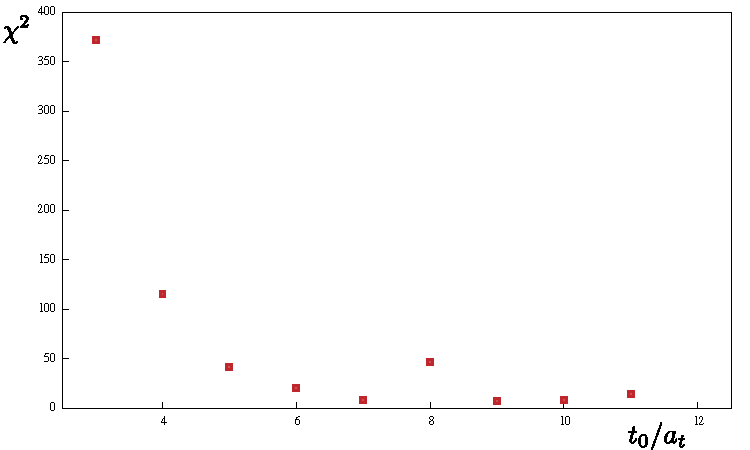
\includegraphics[width=0.8\linewidth]{figures/ChisquareT1mP/chisquare.pdf}
%\caption{ A $\chi^2$-like quantity in the $\Lambda^{PC} = T_1^{--}$ irrep for isovector correlators. \label{fig::ChisqT1mP} {\color{red} update to $A_1^{-+}$}}. 
%\end{centering}
%\end{figure}
%
%
%{\color{blue} RECONSTRUCTION PLOTS AND MORE WORDS}

 
 
%%%%%%%%%%%%%%%%%%%%%%%%%%%%%%%%%%%%%%%%%%%%%%%%%%%%%%%%%
%%%%%%%%%%%%%%%%%%%%%%%%%%%%%%%%%%%%%%%%%%%%%%%%%%%%%%%%%
%%%%%%%%%%%%%%%%%%%%%%%%%%%%%%%%%%%%%%%%%%%%%%%%%%%%%%%%%


\subsection{Principal Correlators} \label{sec::Spec:corrConstructPcorr}
The actual details of the implementation of our variational solution in terms of Singular Value Decomposition is discussed along with the derivation in \appref{app::GEVP}. We now turn to the details of spectral extraction from the \emph{principal correlators}, $\lambda_{\estate{n}}(t)$. The principal correlators can be shown by perturbation theory \cite{Blossier:2009kd} to behave asymptotically like
\begin{equation*}
\lambda_{\estate{n}}(t) \sim e^{-E_\mathfrak{n}(t-t_0)} + \mathcal{O}(e^{-E_{\estate{N+1}}t}).
\end{equation*}
Here, for a basis of $N$ operators, $E_{\estate{N+1}}$, is the energy of the $N+1$'th state.  The corrections, as expected, are proportional to the exponentiation of the energies of states that lie outside the reach of our variational basis, the smallest of which produces the largest correction. 

In practice we fit the principal correlators to the form 
\begin{equation*}
\lambda_{\estate{n}}(t) = (1-A_{\estate{n}})e^{-E_\estate{n}(t-t_0)} + A_{\estate{n}}e^{-E'_\estate{n}(t-t_0)}
\end{equation*}
where the fit parameters are $A_{\estate{n}}$, $E_{\estate{n}}$, and $E'_{\estate{n}}$. The second exponential term is present to help stabilize the fit and allows us to consider the behavior of the principal correlator at smaller times. We require the energy of the second exponential, $E'_\estate{n}$ to be larger than  $E_\estate{n}$ typically finding in practice that $E'_\estate{n}$ is of roughly the same size as $E_\estate{N}$ (i.e. it is of the size of the energy of states lying just outside the reach of our basis of operators). 

We plot a subset of principal correlators, extracted in this analysis, along with their fits, in the left and right panels of  \figref{fig::PcorrLevel}. The dominant time dependence, due to state $\estate{n}$, has been divided out such that the correlator becomes flat at the point the fit becomes dominated by the single state of interest. Empirically the importance of the second exponential becomes smaller as one increases the value of $t_0$. Further, in agreement with the perturbative analysis, the mass scale of the second exponential becomes larger than $E_\estate{N}$, $\estate{N} = \mathrm{dim}(C)$. At too early values of $t_0$ this is not necessarily true, and indication that we are forcing an incorrect orthogonality relation as discussed previously. 

\afterpage{
 \begin{figure}[htbp]
\begin{centering}
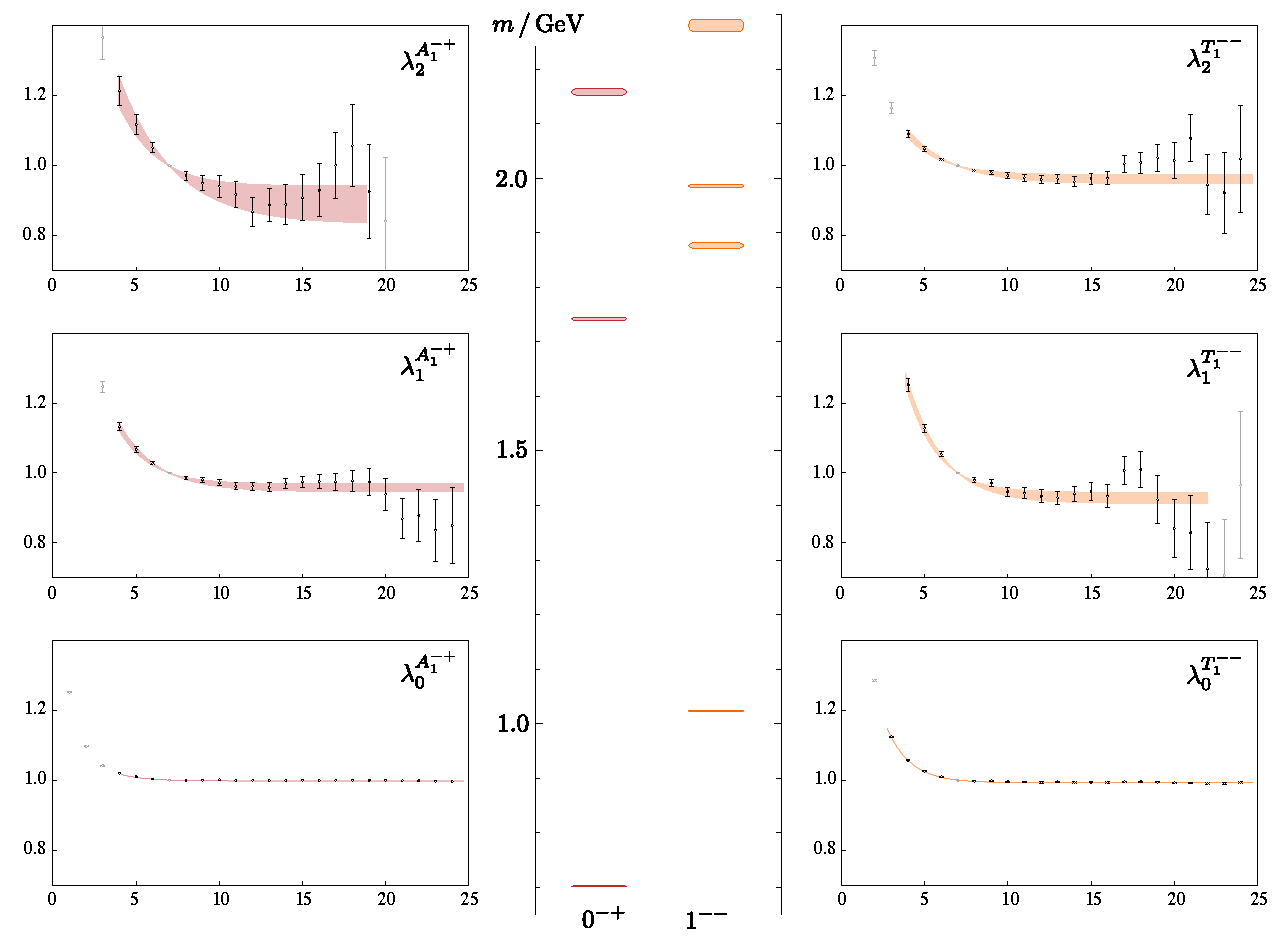
\includegraphics[width=\linewidth]{figures/PrinCorrT1mPA1mM/LevelDiagramWithT1mP_A1mM_PCorrs.pdf}
\caption{ Principal Correlators in the  $\Lambda^{PC} = A_1^{-+}$ and $T_1^{--}$ irreps containing $J^{PC}= 0^{-+}$ and $1^{--}$ mesons. We plot $e^{E_{\mathfrak{n}}(t-t_0)}\lambda_{\mathfrak{n}}(t)$. \label{fig::PcorrLevel}}
\end{centering}
\end{figure}
\clearpage
}



%%%%%%%%%%%%%%%%%%%%%%%%%%%%%%%%%%%%%%%%%%%%%%%%%%%%%%%%%
%%%%%%%%%%%%%%%%%%%%%%%%%%%%%%%%%%%%%%%%%%%%%%%%%%%%%%%%%
%%%%%%%%%%%%%%%%%%%%%%%%%%%%%%%%%%%%%%%%%%%%%%%%%%%%%%%%%


\subsection{Continuum Symmetries} \label{sec::Spec:corrConstructContSym}
As discussed previously, it should be possible through appropriate smearing, construction of operators with good continuum symmetry, and a reduction of discretization effects via improvements to the action and a sufficiently fine mesh, to restore continuum rotational symmetry to a good approximation with only small deviations. We do in fact see this apparent restoration in our lattice calculations. In \figref{fig::RotSymT1mP} we plot a correlation matrix for $\Lambda^{PC} = T_1^{--}$, organized by the continuum spin-$J$ of each operator, and normalized such that the diagonal elements are unity. We see, in explicit calculation, a nearly block diagonal matrix, an indication that the underlying continuum symmetry is approximately restored. 

\afterpage{
 \begin{figure}[htbp]
\begin{centering}
\includegraphics[width=0.8\linewidth]{figures//EmergentRotationalSymmetryT1mP/MatrixPlotLabelsCrop.pdf}
\caption{ Approximate restoration of rotational symmetry in the $\Lambda^{PC} = T_1^{--}$ irrep. We plot the normalized correlation matrix, $|C_{ij}/\sqrt{C_{ii}C_{jj}}|$ on timeslice 5. Operators subduced from spin 1 appear first followed by those subduced from spin 3 and then spin 4. \label{fig::RotSymT1mP}}
\end{centering}
\end{figure}
\clearpage
}

%%%%%%%%%%%%%%%%%%%%%%%%%%%%%%%%%%%%%%%%%%%%%%%%%%%%%%%%%
%%%%%%%%%%%%%%%%%%%%%%%%%%%%%%%%%%%%%%%%%%%%%%%%%%%%%%%%%
%%%%%%%%%%%%%%%%%%%%%%%%%%%%%%%%%%%%%%%%%%%%%%%%%%%%%%%%%


\subsection{State Identification} \label{sec::Spec:corrConstructStateIdent}

\afterpage{
 \begin{figure}[htbp]
\begin{centering}
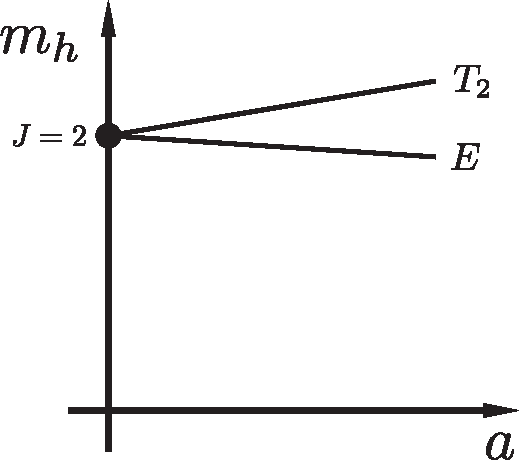
\includegraphics[width=0.3\linewidth]{figures/ContinuumExtrapolationMass/ContinuumExtrapolation.pdf}
\caption{A toy continuum limit on a $J=2$ meson. In general the extrapolation to the continuum limit may also include higher powers of the lattice spacing $a$.  \label{fig::contExtrapMass}}
\end{centering}
\end{figure}
\clearpage
}

Having identified an approximate restoration of rotational symmetry we can ask the question ``Can we identify the continuum $J^{PC}$ quantum numbers of a state from our lattice calculation?" Formally the most rigorous method to determine the spin of a state would be to perform a set of lattice calculations on successively finer meshes and then extrapolate the result to the continuum limit in which the discretization is removed. Such an extrapolation would involve a fit of the lattice masses to a function that is polynomial in $a$, the lattice spacing. One expects that after performing such a fit patterns of degeneracies would emerge, according to the patterns of subduction, and the result would be free of the discretization effects present in any single calculation. For example a spin-2 meson would appear as a degenerate set of energies in the $T_2$ and $E$ irreps (as in \figref{fig::contExtrapMass}), a spin-3 state as a degeneracy across $T_1$, $T_2$, and $A_2$, and so on. Such extrapolations have indeed been performed in pure gauge theory, $SU(3)$ Yang-Mills Theory, in the extraction of the low-lying glueball spectrum  \cite{Morningstar:1999rf}. 

\afterpage{
\begin{figure}[htbp]
\begin{centering}
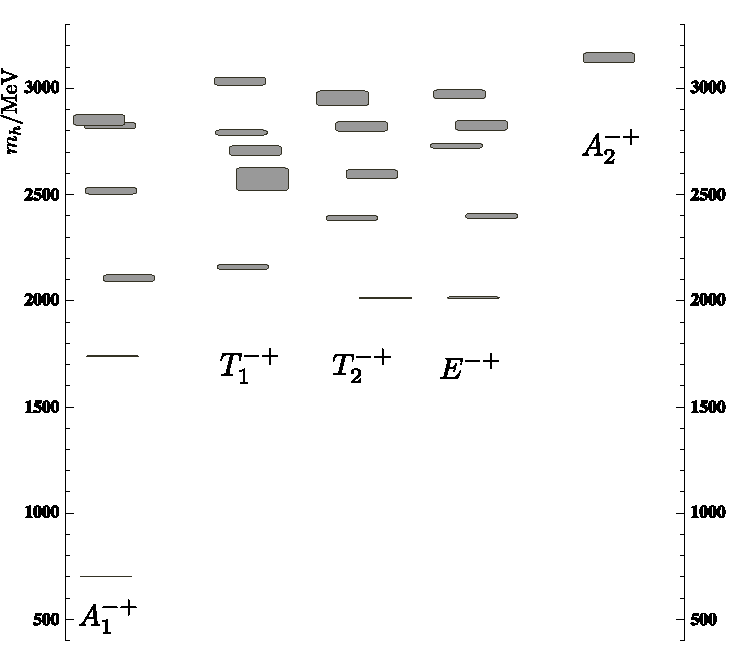
\includegraphics[width=0.8\linewidth]{figures/LatticeSpectrum743/BoxPlotUnlabeledmM.pdf}
\caption{ $\Lambda^{PC} = (A_1,T_1,T_2,E,A_2)^{-+}$ $SU(3)_F$ spectrum. \label{fig::LatticemMSpec743Raw}}
\end{centering}
\end{figure}
\clearpage
}

This procedure, applied to hadrons, is more complicated. Firstly it relies on a series of calculations on finer and finer meshes and thus comes at a large computational cost. Additionally one must simulate at a fixed quark mass, a quantity which has non-trivial dependence on the lattice spacing, thus one has complications associated with generating the required lattices beyond just the price tag. Even more troublesome however is the degree of near degeneracy manifest in the continuum spectrum when organized in terms of $J^{PC}$. When we move to the lattice the problem of degeneracy is vastly magnified, we exchange an infinite number of irreducible representations, spin-J, for the finite number of irreps of the cube. This means that the extracted spectrum becomes significantly more dense and would require statistical precision beyond that which we show here\footnote{The prototypical example of the difficulty in level identification comes from considering the subduction patterns of a $J^{PC} = 4^{++}$ meson. The fingerprint of such a continuum state would be nearly degenerate energy levels lying in $(A_1,T_1,T_2,E)^{++}$. This fingerprint is not however unique. $J^{PC} = (0,1,2)^{++}$, corresponding to a $^3P_J$ multiplet would have the same pattern. Further, on the basis of the quark model outlined earlier, we would also expect these states to also be nearly degenerate.} .  

In order to demonstrate the density of states in any given irrep we plot the spectrum of states obtained by considering $\Lambda^{PC} = (A_1,T_1,T_2,E,A_2)^{-+}$ mesons in \figref{fig::LatticemMSpec743Raw}. While the ground states in any given channel are readily identified we see the spectrum becomes fairly dense once one considers excited states. The calculation we present is performed at the $SU(3)_F$ point where all of the quarks are tuned approximately to the strange quark mass. 

%Further, this calculation is being performed at the $SU(3)_F$ point where all of the quarks are tuned approximately to the strange quark mass. %As one moves toward the physical point the constituent $u$ and $d$ quarks become lighter, multi-particle states become important, and the spacing between levels begins to shrink. 

To alleviate the difficulties with spin identification it would be useful to have a procedure which is effective at only a single spacing. This spacing should be fine enough that the spectrum exhibits, to a sufficient degree, the underlying rotational symmetry present in QCD. As shown in \figref{fig::RotSymT1mP} the lattices we employ, coupled with appropriate smearing and operator construction, appear to manifest the requisite underlying symmetry. 

The procedure, first demonstrated in \cite{Dudek:2009qf}, which we employ, makes use of both the spectrum and the operator state overlaps,  $Z_i^{\estate{n}} \equiv \langle \estate{n} | \mathcal{O}^\dagger_i | 0 \rangle$, to identify the continuum $J^{PC}$ quantum numbers. As mentioned previously, our operator basis is constructed to fully respect cubic symmetry. However, from \figref{fig::RotSymT1mP}, it is also apparent that these operators contain a `memory' of the continuum spin from which they were subduced\footnote{If they did not there would be no block diagonal sub structure in  \figref{fig::RotSymT1mP}.}.  The correlation matrix appears to be approximately block diagonal when the operators are ordered according to the spin from which they were subduced. %\footnote{In the case of $J=4$, featuring three derivatives, the symmetry is not as good. Two and three derivative operators are dimension 5 and 6 respectively, under renormalization these higher mass dimension operators can mix with lower mass dimension operators generating effects that scale like the inverse of the lattice spacing. These renormalization artifacts, while present, are not so large as to spoil the method. We expect that the use of smeared fields suppressed these dimensional mixings as they are most sensitive to the high energy physics that smearing removes. The lattice only serves to regulate the quantum field theory; renormalization must be dealt with separately.}. 

Motivated by the block diagonal nature of the correlation matrix we propose to use the operator overlaps, $Z_i^{\estate{n}} \equiv \langle \estate{n} | \mathcal{O}^\dagger_i | 0 \rangle$, in order to assign, to each state in our spectrum, an integer continuum spin, $J$. 

The essence of the method relies on the observation that operator overlaps should be degenerate in each irrep up to discretization artifacts. Our operators are constructed to be of definite spin, $\langle 0 | \mathcal{O}^{J,M} | J',M' \rangle = Z^{[J]}\delta_{J,J'}\delta_{M,M'}$ from which it follows\footnote{For a sufficiently fine discretization one might imagine that the cubic degrees of freedom are an approximate relabeling of the continuum spin degrees of freedom, $| \Lambda, \mu \rangle \approx \sum_{M} S^{J,M}_{\Lambda,\mu} | J, M\rangle$. } that  $\langle 0 | \mathcal{O}^{[J]}_{\Lambda,\mu} | \Lambda',\mu' \rangle \approx S^{J,M}_{\Lambda,\mu}S^{J',M*}_{\Lambda',\mu'}Z^{[J]}\delta_{J,J'} \approx Z^{[J]}\delta_{\Lambda,\Lambda'}\delta_{\mu,\mu'}$. Spin-J states should have the same operator overlap up to small deviations. 

This sort of logic, states overlapping dominantly onto a single spin, is indeed present in explicit calculation. In \figref{fig::StateIdentT2mP} we plot the unit normalized overlap for a hierarchy of extracted masses in the $T_2^{--}$ irrep corresponding to spin $J=2,3,4,\ldots$ mesons. 

\afterpage{
\begin{figure}[htbp]
\begin{centering}
\includegraphics[height=0.6\textheight]{figures/state_ident_T2mP/StateIdent_crop.pdf}
\caption{ State identification in the $\Lambda^{PC} = T_2^{--}$ irrep. Each operator has been normalized, across states, so that $\langle 0 | \mathcal{O}_{T_2} | \estate{n}; T_2 \rangle$ takes a maximal value of one.   \label{fig::StateIdentT2mP}}
\end{centering}
\end{figure}
\clearpage
}

In order to make use of this information we should also show that we do observe the degeneracy previously outlined. This conjectured degeneracy of both masses and operator overlaps is indeed observed in our lattice calculations \cite{Dudek:2010wm,Dudek:2009qf}.  In \figref{fig::J4mMDegen} we show a pattern of  degenerate masses and operator overlaps across the $\Lambda^{PC} = (A_1,T_1,T_2,E)^{-+}$ irreps consistent with a spin-4 meson. We plot the state overlaps with the three derivative operator\footnote{The symbol  $D^{[3]}_{2,3}$ means `construct a three derivative operator, couple the outer two derivatives into $J=2$, then couple the third derivative to make $J=3$'.}
\begin{equation*}
\mathcal{O} \sim  (\epsilon_{ijk} \gamma_i\gamma_j \times D^{[3]}_{2,3})^{J=4} .
\end{equation*}
This is to say an operator in which three gauge covariant derivatives are coupled together to form spin-3 which is then combined with a positive parity vector gamma matrix structure to form $J^{PC} = 4^{-+}$. In all four irreps we find that the tentatively identified $J^{PC}=4^{-+}$ state overlaps predominantly with this operator. Further, we find that the extracted masses and overlaps are statistically compatible across each irrep and indicating the observation of a spin-4 meson. 

\afterpage{
\begin{figure}[htbp]
\begin{centering}
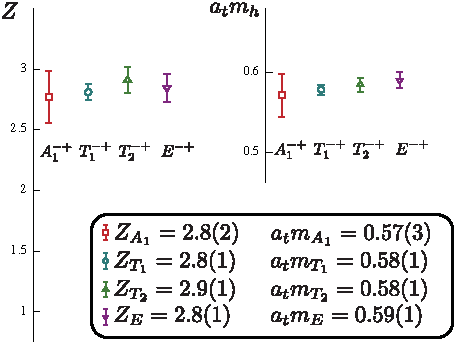
\includegraphics[width=0.8\linewidth]{figures/operator_overlap_degeneracy_J4mM/Degeneracy2.pdf}
\caption{ Degeneracy patterns in the $\Lambda^{PC} = (A_1,T_1,T_2,E)^{-+}$ irreps.\label{fig::J4mMDegen}}
\end{centering}
\end{figure}
\clearpage
}

Turning now to the state identification, the procedure proceeds by identifying the dominant $J$ overlapping with each state. Returning to  \figref{fig::StateIdentT2mP} we explicitly demonstrate the efficacy of our  procedure using a subset of the available operators corresponding to the most relevant constructions. Read, along any single histogram, from top to bottom, the operators are 
% \begin{align*}
%rho_a1xD1_J1__J2_T2 1 0 * \\
%rho_a1xD3_J132_J3__J2_T2 1 0 * \\
%rho_b1xD3_J131_J1__J2_T2 1 0 * \\
%rho_rho_2xD2_J2__J3_T2 1 0 * \\
%rho_a1xD3_J132_J3__J3_T2 1 0 * \\
%rho_b1xD3_J131_J2__J3_T2 1 0 * \\
%rho_a1xD3_J132_J3__J4_T2 1 0 
%\end{align*}
\begin{align*}
\mathcal{O}_{T_2}^{(1),[J=2]} &\sim \left( \gamma_5\gamma_k \times D^{[1]} \right)^{J=2}   \\
\mathcal{O}_{T_2}^{(2),[J=2]} &\sim  \left( \gamma_5\gamma_k \times D^{[3]}_{2,3}\right)^{J=2}   \\
\mathcal{O}_{T_2}^{(3),[J=2]} &\sim  \left( \epsilon_{ijk} \gamma_i\gamma_j \times D^{[3]}_{1,1} \right)^{J=2}   \\
\mathcal{O}_{T_2}^{(4),[J=3]} &\sim  \left( \gamma_0 \gamma_k \times D^{[2]}_2 \right)^{J=3}  \\
\mathcal{O}_{T_2}^{(5),[J=3]} &\sim  \left( \gamma_5\gamma_k \times D^{[3]}_{2,3} \right)^{J=3}   \\
\mathcal{O}_{T_2}^{(6),[J=3]} &\sim  \left( \epsilon_{ijk} \gamma_i\gamma_j \times D^{[3]}_{1,2}\right)^{J=3}   \\
\mathcal{O}_{T_2}^{(7),[J=4]} &\sim  \left( \gamma_5\gamma_k \times D^{[3]}_{2,3}\right)^{J=4} .  
\end{align*}

We find, as might be expected assuming that rotational symmetry is approximately restored, that each state appears to have dominant overlap onto only a single spin. The other irreps, both at rest and in flight, also exhibit similar behavior. By repeating this procedure, identifying the dominant spin component of each state in each irrep, we are able to find the patterns of degenerate states in our lattice calculation. We reproduced the spin identified spectra, for the lowest set of isovector mesons, in Figures \ref{fig::LatticemMSpec743SpinIdent}, \ref{fig::LatticemPSpec743SpinIdent}, \ref{fig::LatticepMSpec743SpinIdent}, and \ref{fig::LatticepPSpec743SpinIdent}. Across each of these plots vertical ellipses represent additional states, present in the spectrum, but whose spin we were unable to unambiguously identify.

%\footnote{The signals for these highly excited states decay rapidly and are often noisy even in the face of the extensive suite of variational tools we have at out disposal.}. 

\afterpage{
\begin{figure}[htbp]
\begin{centering}
\includegraphics[width=\linewidth]{figures/LatticeSpectrum743/BoxPlotLabeledmM_crop.pdf}
\caption{ Spin identified $J^{PC} = J^{-+}$ $SU(3)_F$ spectrum. \label{fig::LatticemMSpec743SpinIdent}}
\end{centering}
\end{figure}
\clearpage
}

\afterpage{
\begin{figure}[htbp]
\begin{centering}
\includegraphics[width=\linewidth]{figures/LatticeSpectrum743/BoxPlotLabeledmP_crop.pdf}
\caption{ Spin identified $J^{PC} = J^{--}$ $SU(3)_F$ spectrum. \label{fig::LatticemPSpec743SpinIdent}}
\end{centering}
\end{figure}
\clearpage
}

\afterpage{
\begin{figure}[htbp]
\begin{centering}
\includegraphics[width=\linewidth]{figures/LatticeSpectrum743/BoxPlotLabeledpM_crop.pdf}
\caption{ Spin identified $J^{PC} = J^{++}$ $SU(3)_F$ spectrum. \label{fig::LatticepMSpec743SpinIdent}}
\end{centering}
\end{figure}
\clearpage
}

\afterpage{
\begin{figure}[htbp]
\begin{centering}
\includegraphics[width=\linewidth]{figures/LatticeSpectrum743/BoxPlotLabeledpP_crop.pdf}
\caption{ Spin identified $J^{PC} = J^{+-}$ $SU(3)_F$ spectrum. \label{fig::LatticepPSpec743SpinIdent}}
\end{centering}
\end{figure}
\clearpage
}
%%%%%%%%%%%%%%%%%%%%%%%%%%%%%%%%%%%%%%%%%%%%%%%%%%%%%%%%%
%%%%%%%%%%%%%%%%%%%%%%%%%%%%%%%%%%%%%%%%%%%%%%%%%%%%%%%%%
%%%%%%%%%%%%%%%%%%%%%%%%%%%%%%%%%%%%%%%%%%%%%%%%%%%%%%%%%

\section{$SU(3)_F$ Spectrum} \label{sec::Spec:results}

We conclude this chapter by presenting the spin identified $SU(3)_F$ spectrum.  

\afterpage{
\begin{figure}[htbp]
\begin{centering}
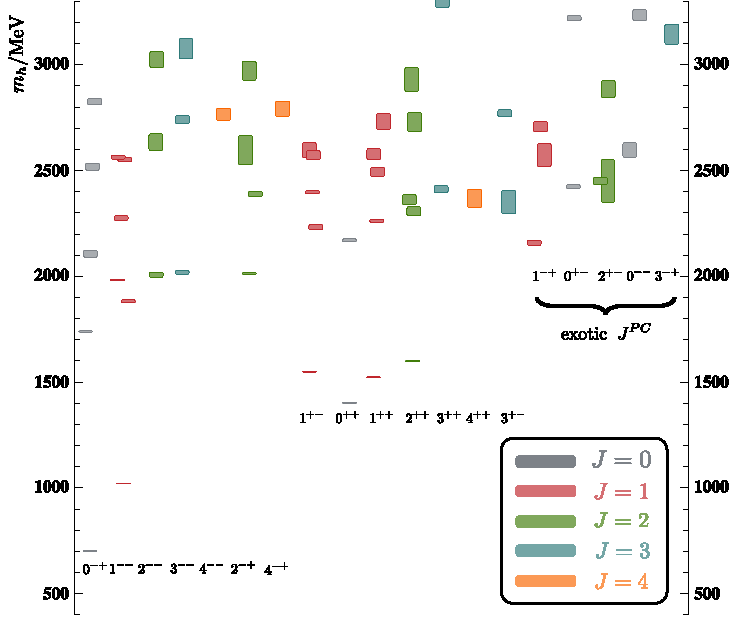
\includegraphics[width=\linewidth]{figures/LatticeSpectrum743/SpinIdentAll.pdf}
\caption{ Spin identified $J^{PC}$ $SU(3)_F$ spectrum. \label{fig::LatticeSpec743SpinIdent}}
\end{centering}
\end{figure}
\clearpage
}


\chapter{Radiative Transitions on the lattice} \label{chap::radTranLattice}

In this chapter we first introduce radiative transition matrix elements and show how they can be decomposed into kinematic factors, transforming with the symmetries of the vector current, multiplying scalar form factors which encode the dynamics of the transition. On the lattice these matrix elements are encoded in three-point functions which feature a local vector current insertion appearing between mesonic creation and annihilation operators. 

By performing a spectral decomposition of the three-point functions, we will find, in a manner similar to our two point calculation,  that any three-point function in principle contains contributions from all states that have the same quantum numbers as the source and sink operators. Each contribution will propagate through Euclidean time and contribute a factor of $e^{-Et}$ such that for large times only the lightest state survives. In general we will also be interested in the excited state matrix elements, their contributions arising from subleading exponentially damped contributions. We circumvent the problem via the use of `optimal' operators. These optimal operators are constructed as linear combinations of operators within our basis. We will show they do in fact dominantly produce a \emph{single} state, and further, that their use in three-point function allows for the non-perturbative determination of matrix elements featuring \emph{excited states} at both the source and sink.

%%%%%%%%%%%%%%%%%%%%%%%%%%%%%%%%%%%%%%%%%%%%%%%%%%%%%%%%%
%%%%%%%%%%%%%%%%%%%%%%%%%%%%%%%%%%%%%%%%%%%%%%%%%%%%%%%%%
%%%%%%%%%%%%%%%%%%%%%%%%%%%%%%%%%%%%%%%%%%%%%%%%%%%%%%%%%

\section{Form-factors and Transitions \label{sec::formfactor}}

The theoretical object we wish to extract is the matrix element, 
\begin{equation}
\langle h'_{J'}(\vec{p}\,',\lambda')|j^\mu | h_J(\vec{p},\lambda) \rangle, 
\end{equation}
 which describes the vector current transition of a spin-$J$, helicity projection $\lambda$, hadron, $h$, to another spin-$J'$, helicity projection $\lambda'$, hadron ,$h'$. The photon couples to the quark fields \footnote{In this calculation we use a non-physical version of QCD in which there are three as opposed to six flavors. Each quark flavor is tuned to approximately the physical strange quark mass such that there is an exact $SU(3)$ flavor symmetry.} within the hadrons (up to a factor of e) via the vector current, $j^\mu = \frac{2}{3}\bar{u}\gamma^\mu u -\frac{1}{3}\bar{d}\gamma^\mu d -\frac{1}{3}\bar{s}\gamma^\mu s $.  
 
 The matrix elements are related to the helicity amplitude for the process $h\rightarrow h'\gamma$ via the inclusion of the final state photon polarization vector, 
 \begin{equation*}
 \mathcal{M}\Big(h(\vec{p},\lambda)\rightarrow h'(\vec{p}\,',\lambda')\gamma(\vec{q},\lambda_\gamma)\Big) = \epsilon_\mu^*(\vec{q},\lambda_\gamma)\langle h'_{J'}(\vec{p}\,',\lambda')|j^\mu | h_J(\vec{p},\lambda) \rangle.
 \end{equation*}
 where $\vec{q} = \vec{p}\,'-\vec{p}$ and the photon has virtuality $Q^2 = |\vec{q}|^2 - \left( E_{h'}(\vec{p}\,') - E_h(\vec{p})\right)^2$. 
 
 In general one writes the matrix element as a sum over products of kinematic factors, transforming with the symmetries of the current, times an unknown coupling which is a function of the photon virtuality, the form factor. For example when one calculates the form factor of a pseudoscalar meson such as the pion a convenient parameterization of the matrix element is 
\begin{equation*}
\langle \pi^+ (p^\prime) | j^\mu | \pi^+ (p) \rangle = \left( p^\prime + p\right)^\mu F_\pi(Q^2).
\end{equation*}
Here the kinematic factor is $\left( p^\prime + p\right)^\mu$ which transforms under parity in the same way as the matrix element. The careful reader will realize that there is another independent kinematic factor which could appear in the decomposition, namely, $  \left( p^\prime - p\right)^\mu F^{[-]}_\pi(Q^2) $, which also transforms correctly under rotations and parity. This quantity can be eliminated via the constraint imposed from current conservation.

In this analysis we consider formfactors and transitions between meson states of integer angular momentum $J$. Form-factors are accessed via vector current matrix elements in which the current appears sandwiched between meson states  that have been projected onto definite momentum $\vec{p}$ and helicity $\lambda$.  A general parameterization of such a matrix element is 

\begin{equation}
\langle h'_{J'}(\vec{p}\,',\lambda')|j^\mu | h_J(\vec{p},\lambda) \rangle = \sum_i K^\mu_i(J^\prime,\vec{p}\,',\lambda';J,p,\lambda)F_i(Q^2) \label{eqn::genericDecompositionHelicity}
\end{equation}
where $K^{\mu}_i$ is a kinematic factor which transforms in the same way as the matrix element. 
%%%%%%%%%%%%%%%%%%%%%%%%%%%%%%%%%%%%%%%%%%%%%%%%%%%%%%%%%
%%%%%%%%%%%%%%%%%%%%%%%%%%%%%%%%%%%%%%%%%%%%%%%%%%%%%%%%%
%%%%%%%%%%%%%%%%%%%%%%%%%%%%%%%%%%%%%%%%%%%%%%%%%%%%%%%%%
\subsection{Vector current matrix elements} \label{ssec::RadTranLat::Decomp}

We adopt a straightforward approach in which we write down the most general Lorentz covariant and parity invariant decomposition of a vector current matrix element in terms of a number of arbitrary form factors. It is convenient in this approach to use the $z$-component of the spin which is not in general equal to the helicity and which we denote by $r$. The choice of using $j_z$ makes the transformation properties of the polarization tensors simpler, one can derive a similar result using a helicity representation. As an illustrative example we demonstrate the method for a pseudoscalar-vector transition relevant to a process such as $\rho \rightarrow \pi \gamma$.   The most general set of kinematic factors one could write down for such a transition is 

\begin{align*}
\langle P(p^\prime) | j^\mu | V(p,r) \rangle &= A_1(Q^2) \epsilon^\mu(p,r)p_+^\alpha q_\alpha \\
&+A_2(Q^2) p_+^\mu \epsilon_\alpha(p,r)q^\alpha \\
&+A_3(Q^2) q^\mu \epsilon_\alpha(p,r) p_+^\alpha \\
&+B_1(Q^2) \epsilon^{\mu\nu\rho\sigma}\epsilon_\nu(p,r)p_{+\rho}q_\sigma
\end{align*}
In which we have chosen to use the basis $p_+ = p^\prime + p$, and $q = p^\prime -p$ for the momenta. $\epsilon_\alpha(p,r)$ represents a polarization vector for a spin-1 particle with momentum $p$ and spin projection $r$. 

Parity invariance requires that 
\begin{align*}
\langle P(p^\prime) | j^\mu | V(p,r) \rangle &= \langle P(p^\prime) | \mathcal{P}^{-1}\mathcal{P} j^\mu  \mathcal{P}^{-1}\mathcal{P}  | V(p,r) \rangle  \\
&= \left[ \mathcal{P} \right]^\mu_\nu \langle P(-p^\prime) | j^\mu | V(-p,r) \rangle
\end{align*}

Where we have used the fact that under parity our states transform as $\mathcal{P} | P(p,r)\rangle = -|P(-p,r)\rangle $, $\mathcal{P} | V(p,r)\rangle = -|V(-p,r)\rangle $, and $\mathcal{P} j^\mu\mathcal{P}^{-1}  = \left[ \mathcal{P}^{-1} \right]^\mu_\nu j^\nu$ \footnote{  \unexpanded{$ \left[ \mathcal{P}^{-1} \right]^\mu_\nu  = \left[ \mathcal{P} \right]^\mu_\nu  = \mathrm{diag}(+---)$ } } . Using the fact that $\epsilon^\mu(-p,r) = - \left[\mathcal{P}\right]^\mu_\nu \epsilon^\nu(p,r)$ we see that the above decomposition is invariant under parity provided $A_i(Q^2) =0$. 
Current conservation provides an additional constraint on the decomposition, 
\begin{align*} 
&0 = \partial_\mu \langle A(p^\prime,r^\prime) | j^\mu | V(p,r) \rangle \\
\Rightarrow \quad & 0 = q_\mu \langle A(p^\prime,r^\prime) | j^\mu | V(p,r) \rangle
\end{align*}
In this case the kinematic factor vanishes when we dot in the photon momentum, $q_\mu  \epsilon^{\mu\nu\rho\sigma}\epsilon_\nu(p,r)p_{+\rho}q_\sigma = 0$. Using these tools we can build parity invariant Lorentz covariant decompositions of vector current matrix elements for mesons of arbitrary spin at the source and sink. We find 
\begin{align*}
\langle P(p^\prime) | j^\mu | V(p,r) \rangle =B_1(Q^2) \epsilon^{\mu\nu\rho\sigma}\epsilon_\nu(p,r)p_{+\rho}q_\sigma
\end{align*}

More generally there can be more than one form factor occurring in such a decomposition\footnote{For example a vector particle has three form factors.}. In this case there is some ambiguity associated with the decomposition. As a first example we can consider the variables used, for example $p$ and $p^\prime$ are an equally valid set of variables to use in the decomposition (as opposed to our choice of $p_+$ and $q$) but would lead to a different normalization of the form-factor $B_1(Q^2)$. In the case of multiple form factors one is also free to perform a linear transformation on the $K^{\mu}_i$ as $\tilde{K}^\mu_i = L_{ij}K^\mu_j$, which in turn causes a redefinition of the $F_i$. Further in the case that one wants to compare results between two different calculations using different bases it is necessary to construct the mapping, $L$, which in the case of several form-factors becomes algebraically cumbersome.
 
A conventional parameterization for the matrix elements is the Multipole Expansion introduced earlier in \chapref{chap::QM}. For convenience of calculation we work with an arbitrary set of form-factors which we then eliminate in favor of the multipole form-factors where appropriate. This is done in direct analogy with \cite{Durand:1962zza,Dudek:2009kk}.

We now proceed to sketch the derivation\footnote{A more complete description can be found in \cite{Durand:1962zza}}. Defining the vertex function in the Breit frame ($\vec{p} = |p|\hat{z}$ , $\vec{p^\prime} = -\vec{p}$) 
\begin{align*}
\Gamma_{J^\prime\lambda^\prime;J\lambda}^\nu &= \langle J^\prime \lambda^\prime p^\prime | e^{i \pi J_2} j^\nu | J \lambda  p\rangle = \langle J^\prime \lambda^\prime| e^{i\xi_{p^\prime} K_3} e^{i \pi J_2} j^\nu e^{-i\xi_p K_3}  | J \lambda  \rangle
\end{align*}
where the operator $e^{-i\xi_p K_3}$ acting on a rest state effects to boost the state along the $z$-axis to momentum $p\hat{z}$. One can show that this matrix element can be reexpressed as a sum over matrix elements of tensors which transform irreducably under the rotation group -- this is the essence of the multipole decomposition. Each tensor appearing in the decomposition also independently satisfies the Wigner-Eckart Theorem allowing us to solve for the reduced matrix elements which we identify as the various multipole moments of the system. Our construction is identical to Durand's and we refer the reader to \cite{Durand:1962zza} for further details. 

The longitudinal and transverse components\footnote{Here longitudinal refers to the helicity zero polarization state which appears for virtual photons while transverse means the plus/minus helicity projections.} of the vector current transform differently under rotations and one must allow for a different set of reduced matrix elements for each. In the Breit frame the scalar and $z$ component are linked through current conservation as $(E^\prime - E ) \Gamma_{J^\prime\lambda^\prime;J\lambda}^0 = -2p_z \Gamma_{J^\prime\lambda^\prime;J\lambda}^3$ and one can reconstruct the charge moments using only the scalar portion of the vertex function as
\begin{equation}
 \Gamma_{J^\prime\lambda^\prime;J\lambda}^0 = \left(-1\right)^{2J^\prime} \sum_k \begin{pmatrix} 
 J^\prime & k & J \\
 \lambda^\prime & 0 & \lambda 
 \end{pmatrix} \langle J^\prime || T^k_0 || J \rangle  \bigg|_{(-1)^k = \delta P}
\end{equation}
where the variable $\delta P$ is the product of the initial and final parities. A similar expression for the transverse components may be derived, one obtains 

\begin{equation}
 \Gamma_{J^\prime\lambda^\prime;J\lambda}^\pm = \left(-1\right)^{2J^\prime} \sum_{k=1}
  \begin{pmatrix} J^\prime & k & J \\
 \lambda^\prime & \pm 1 & \lambda  \end{pmatrix} 
 \langle J^\prime || T^k_\pm || J \rangle  .
\end{equation}

We note that in the case of identical particles the sum ocurring above is restriced to odd values of $k$. A conventional redefinition of the reduced matrix elements is 
\begin{align*}
 \langle J^\prime || T^k_\pm || J \rangle &= \frac{1}{2}\left[ \left(1 + (-1)^k\delta P\right)E_k + \left(1 - (-1)^k \delta P \right)  M_k  \right] \\
  \langle J^\prime || T^k_0 || J \rangle &= \frac{1}{2} \left(1 + (-1)^k\delta P\right)C_k 
\end{align*} 
where E(M)[C] indicate electric(magnetic)[charge] multipole elements.  

Returning now to our pseudoscalar-vector example we see that $B_1(Q^2)$ can be identified as a magnetic dipole ($M_1$) form factor. More generally there can be multiple form factors occurring in any decomposition, each form factor being a linear combination of the multipoles occurring above. One procedure, which allows for efficient conversion between multipole form factors and some arbitrary basis, is to use the equations above to build a linear system, featuring both sets of formfactors, which can be inverted in order to convert to the multipole basis. 

%%%%%%%%%%%%%%%%%%%%%%%%%%%%%%%%%%%%%%%%%%%%%%%%%%%%%%%%%
%%%%%%%%%%%%%%%%%%%%%%%%%%%%%%%%%%%%%%%%%%%%%%%%%%%%%%%%%
%%%%%%%%%%%%%%%%%%%%%%%%%%%%%%%%%%%%%%%%%%%%%%%%%%%%%%%%%
\subsection{Kinematic Decompositions}

Having introduced the technical machinery used to decompose vector current matrix elements we now turn to the decompositions used in this analysis. In particular we will be interested in extracting form factors a transition matrix elements of pseudoscalar and vector mesons. As mentioned previously the form factor decomposition for a pseudoscalar such as the pion may be written as
\begin{equation} \label{eqn::pion_decomp}
\langle \pi^+ (p^\prime) | j^\mu | \pi^+ (p) \rangle = \left( p^\prime + p\right)^\mu F_\pi(Q^2).
\end{equation}

We will also be interested in transitions between two different pseudoscalar particles. Again there is a single form factor, but here the kinematic factor is different due to the difference in mass between the initial and final states. The decomposition we will use is 
\begin{align}\label{eqn::pipip_decomp}
\big\langle \pi'^+ & (\vec{p}\,') \big| j^\mu \big| \pi^+(\vec{p}) \big\rangle = \left[ (p\!+\!p')^\mu \!+\! \tfrac{m'^2 - m^2}{Q^2} (p' \!-\! p)^\mu \right]\!  F_{\pi'\pi}(Q^2). 
\end{align} 

The transition matrix-element between a vector particle and a pseudoscalar can be expressed as\footnote{Note that here we use a slightly different normalization relative to that presented in \secref{ssec::RadTranLat::Decomp}.}
\begin{align}
\big\langle \pi^+(\vec{p}\,') \big| j^\mu \big| \rho^+(\lambda, \vec{p}) \big\rangle  = \epsilon^{\mu \nu \rho \sigma} p'_\nu\, p^{\,}_\rho \,\epsilon^{\,}_\sigma(\lambda, \vec{p}\,) \, \tfrac{2}{m_\pi + m_\rho} F_{\rho \pi}(Q^2),\label{rho_pi_ff}
\end{align} 
and for a vector meson stable under the strong interactions, the transition form-factor at ${Q^2=0}$ can be related to the radiative decay width ${\Gamma( \rho^+ \to \pi^+ \gamma) = \frac{4}{3} \alpha \frac{\lvert \vec{q}\,  \rvert^3}{(m_\rho + m_\pi)^2} \lvert F_{\rho \pi}(0) \rvert^2    }$, where $\vec{q}$ is the momentum of the final-state photon in the rest-frame of the decaying $\rho$ meson.


A vector particle has three form factors once current conservation, parity invariance, and time reversal invariance are demanded  \cite{Arnold:1979cg}. One basis is 
\begin{align}
\big\langle \rho&^+(\lambda',\vec{p}\,') \big| j^\mu \big| \rho^+(\lambda, \vec{p}) \big\rangle \nonumber \\
= 	&- \big[(p+p')^\mu \; \epsilon^*(\lambda',\vec{p}\,') \cdot \epsilon(\lambda,\vec{p}) \big]\; G_1(Q^2) \nonumber \\
	&+ \big[\epsilon^\mu(\lambda,\vec{p}) \, \epsilon^*(\lambda',\vec{p}\,') \!\cdot\! p + \epsilon^{\mu*}(\lambda',\vec{p}\,')\, \epsilon(\lambda,\vec{p})\!\cdot\! p' \big]\, G_2(Q^2) \nonumber \\
	&- \big[(p+p')^\mu \; \epsilon^*(\lambda',\vec{p}\,') \!\cdot\! p \;  \epsilon(\lambda,\vec{p})\!\cdot\! p' \, \tfrac{1}{2m^2} \big]\; G_3(Q^2), \label{eqn::rho_Gi_basis}
\end{align} 
with a corresponding set of three independent dimensionless form-factors $G_1$, $G_2$, $G_3$. A convenient basis having a clearer physical motivation is provided by the expansion of the vector current in terms of multipoles \cite{Durand:1962zza}, which in this case leads to a set of form-factors,
\begin{align}
G_C &= \left(1 + \tfrac{Q^2}{6m^2} \right) G_1 - \tfrac{Q^2}{6m^2} \, G_2 + \tfrac{Q^2}{6m^2} \left(1 + \tfrac{Q^2}{4m^2} \right) G_3 \nonumber \\
G_M &= G_2 \nonumber \\
G_Q &= G_1 - G_2 + \left(1 + \tfrac{Q^2}{4m^2} \right) G_3, \label{eqn::rho_Gmultipole_basis}
\end{align}
which are proportional to the charge ($C_0$), magnetic dipole ($M_1$), and quadrupole ($C_2$) multipoles respectively. At $Q^2=0$ they are related to the charge, magnetic moment and quadrupole moment of the vector meson: $G_C(0) = 1$, $G_M(0) = 2 m\cdot  \mu_\rho$, $G_Q(0) = m^2 \cdot Q_\rho$.

The other form-factors we considered above may also be identified with a particular multipolarity -- in the ${\rho \to \pi \gamma}$ transition case the single form-factor is of magnetic dipole ($M_1$) type, while for the $\pi$ cases it is a charge form-factor  $(C_0)$. The form factors we extract are real functions of $Q^2$. 

%%%%%%%%%%%%%%%%%%%%%%%%%%%%%%%%%%%%%%%%%%%%%%%%%%%%%%%%%
%%%%%%%%%%%%%%%%%%%%%%%%%%%%%%%%%%%%%%%%%%%%%%%%%%%%%%%%%
%%%%%%%%%%%%%%%%%%%%%%%%%%%%%%%%%%%%%%%%%%%%%%%%%%%%%%%%%

\section{Three Point Functions} \label{sec::3ptFun}
Now that we have introduced the objects of interest, vector current matrix elements, and shown how they can be decomposed into form factors encoding the dynamics of hadronic transitions, we can proceed to illustrate how one can apply the machinery of lattice QCD to extract the matrix elements of interest from three-point correlation functions. The essential structure of the correlation functions of interest is 
\begin{equation}
C_{f\mu i}(\Delta t, t) = \langle 0 | \mathcal{O}_f(\Delta t) j_\mu(t) \mathcal{O}_i^\dagger(0) | 0 \rangle. 
\end{equation}
Here the operators, $\mathcal{O}_{f,i}$, are capable of interpolating the mesonic states of interest from the vacuum. Insertion of a complete set of states and performing time evolution of the operators yields, in a manner similar to that presented in \secref{sec::Spec:corrFunc}, a spectral decomposition, 
\begin{align}
C_{f\mu i}(\Delta t, t) = \sum_{\mathfrak{n}_f,\mathfrak{m}_i} \frac{1}{2E_{\mathfrak{n}_f}}\frac{1}{2E_{\mathfrak{m}_i}}e^{-E_{\mathfrak{n}_f}(\Delta t -t)} e^{-E_{\mathfrak{m}_i}t}  \langle 0 | \mathcal{O}_f(0) | \mathfrak{n}_f \rangle \, \langle \mathfrak{n}_f |  j_\mu(0)  | \mathfrak{m}_i \rangle \, \langle \mathfrak{m}_i | \mathcal{O}_i^\dagger(0) | 0 \rangle. 
\end{align}
In this manner we see that the three-point correlation function encodes the matrix element of interest, $ \langle \mathfrak{n}_f |  j_\mu(0)  | \mathfrak{m}_i \rangle$, as well as \emph{all} other transition matrix elements having the same quantum numbers as the source and sink operators. 

Our job now is to determine how we can extract a \emph{single} matrix element from such a correlation function. The summation above runs over all states, but clearly, if the separation between operators is large, $\Delta t >> t >> 0 $, we see that the correlation function will become dominated by the lightest states in the $i$ and $f$ channels. At more modest separations we expect there to be subleading, exponentially suppressed, `pollution' terms which could potentially be a source of systematic error in a calculation interested only in ground state matrix elements. One general feature, present in lattice calculations, is that statistical noise tends to increase with increasing operator separation -- the naive approach of simply pulling the source and sink far apart may not be practical in explicit calculation. 

For our purposes we are also interested in extraction of \emph{excited} state matrix elements whose contribution to the above correlation function is exponentially suppressed. In principle one could attempt to determine the value of these matrix elements via their time dependence but the resolution of such subleading, exponentially suppressed signals proves troublesome in practice.  

%%%%%%%%%%%%%%%%%%%%%%%%%%%%%%%%%%%%%%%%%%%%%%%%%%%%%%%%%
%%%%%%%%%%%%%%%%%%%%%%%%%%%%%%%%%%%%%%%%%%%%%%%%%%%%%%%%%
%%%%%%%%%%%%%%%%%%%%%%%%%%%%%%%%%%%%%%%%%%%%%%%%%%%%%%%%%

\subsection{Optimized Operators} \label{sec::OptOps}

Our solution to this problem is to generate `optimal' operators which dominantly create only a single state in the spectrum. In general a color-singlet operator $\mathcal{O}_i^\dag$ having definite $J^{PC}$ can produce all QCD eigenstates having those quantum numbers,
\begin{equation}
	\mathcal{O}_i^\dag |0\rangle = \sum_\mathfrak{n} \frac{1}{2E_{\mathfrak{n}}} |\mathfrak{n} \rangle \langle \mathfrak{n} | \mathcal{O}_i^\dag |0\rangle.  \nonumber
\end{equation}
We seek to determine optimized interpolators, $\Omega_\estate{n}^\dagger$, which when acting on the vacuum strongly interpolate only a \emph{single} state with much reduced contributions from other states,
\begin{align*}
\Omega_\estate{n}^\dagger | 0 \rangle &= \frac{1}{2E_{\mathfrak{n}}}|\estate{n}\rangle \langle \estate{n} | \Omega^\dagger_\estate{n} | 0 \rangle + \sum_{\estate{m} \neq \estate{n}} \frac{1}{2E_{\mathfrak{m}}}  |\estate{m}\rangle \langle \estate{m} | \Omega^\dagger_\estate{n} | 0 \rangle \\
&=\frac{1}{2E_{\mathfrak{n}}} |\estate{n}\rangle \langle \estate{n} | \Omega^\dagger_\estate{n} | 0 \rangle + \sum_{\estate{m} \neq \estate{n}}  |\estate{m}\rangle \varepsilon_\estate{m}.
\end{align*}
In essence we seek a procedure by which we can minimize the $\varepsilon_\estate{m}$ ($\estate{m} \neq \estate{n}$) relative to the strength with which our operator creates the $\estate{n}$'th state, $\langle \estate{n} | \Omega^\dagger_\estate{n} | 0 \rangle/2E_{\estate{n}}$. 

We will define these optimal operators to be linear combinations of operators within a variational basis. That is operators of generic structure
\begin{equation*}
\Omega_\estate{n}^\dagger = \sum_i w_i^{(\estate{n})} \mathcal{O}_i^\dagger.
\end{equation*}
Returning for a moment to the variational analysis presented in \chapref{chap::Spectroscopy}, we alluded to the fact that the generalized eigenvalue problem we solve, $C(t)v^{(\estate{n})}(t) = \lambda_{\estate{n}}(t) C(t_0) v^{(\estate{n})}(t)$, arises in the context of a variational optimization of the amplitude to create the $\estate{n}$'th state. In the same manner, the best estimate, in a variational sense, for the weights $w_i^{(\estate{n})}$, are the generalized eigenvectors occurring in the generalized eigenvalue problem. We define the optimized operators as 
\begin{equation*}
\Omega_\estate{n}^\dagger = \sqrt{2E_{\estate{n}}}e^{-E_{\estate{n}}t_0/2} \sum_i v_i^{(\estate{n})} \mathcal{O}_i^\dagger,
\end{equation*}
where the coefficient appearing in front of the sum is chosen to give the normalization $\langle \estate{n}| \Omega_\estate{n}^\dagger | 0 \rangle = 2E_{\estate{n}}$. In practice we use the \emph{mean} value of $v_i^{(\estate{n})}$ over the ensemble of gauge configurations to generate the weights. This procedure, of solving the generalized eigenvalue problem in a basis of variational interpolating fields and using the generalized eigenvectors to construct optimal operators, is repeated independently for each quantum number and momentum projection that we will use. 

In order to motivate the use of projected operators we first demonstrate their efficacy in projecting a single state out of a two point correlation function. In \figref{fig::TwoPointRelax} we plot the two point function $\langle 0 | \mathcal{O}(t) \mathcal{O}^\dagger(0) | 0 \rangle$ for $\mathcal{O} = \bar{\psi}\gamma_5\psi, \Omega_\pi$, where the data have been normalized such that they `flatten' to a value of one once the pion dominates the correlation function\footnote{$\bar{\psi}\gamma_5\psi$ is one of the simplest local fermion bilinears that is capable of producing a pion.}. We find that the optimized operator is capable of isolating the pion at significantly earlier times than the fermion bilinear $\bar{\psi}\gamma_5\psi$. 

\afterpage{
\begin{figure}[htbp]
\begin{centering}
\includegraphics[width=0.8\linewidth]{figures/radTrans/TwoPointRelaxation.pdf}
\caption{ Rest frame pion correlator using $\bar{\psi}\gamma_5\psi$ (red) as compared to the optimized operator $\Omega_0$ in blue. We plot $2m_\pi e^{m_\pi t} \langle 0 | \mathcal{O}(t) \mathcal{O^\dagger}(0) | 0 \rangle / | \langle 0 | \mathcal{O} |\pi\rangle | ^2$ \label{fig::TwoPointRelax}}
\end{centering}
\end{figure}
\clearpage
}

In this manner optimized operators can be used to make the calculation of ground state matrix elements more efficient. As mentioned perviously, we aim to move beyond ground state matrix elements. In order to demonstrate the efficacy of our optimized operators, applied to \emph{excited} states, we plot the \emph{effective mass}\footnote{Denoting the two point function $C(t)$, the effective mass is $-\frac{d}{dt} \ln(C(t))$, which is a constant, specifically the mass, provided a single state dominates the two point function, $C(t)\sim Ae^{-mt}$. The derivative is approximated using a forward finite difference derivative.} for the lightest four states in the $A_2^+$ irrep of momentum direction $\vec{p} = \frac{2\pi}{L}[1,0,0]$\footnote{From this point forward we will adopt the convention that we describe momentum using a directional vector of integers, $\vec{n}_{\vec{p}}$, where the momentum is specified via $\vec{p} = \frac{2\pi}{L}\vec{n}_{\vec{p}}$.}.  

\afterpage{
\begin{figure}
\begin{centering}
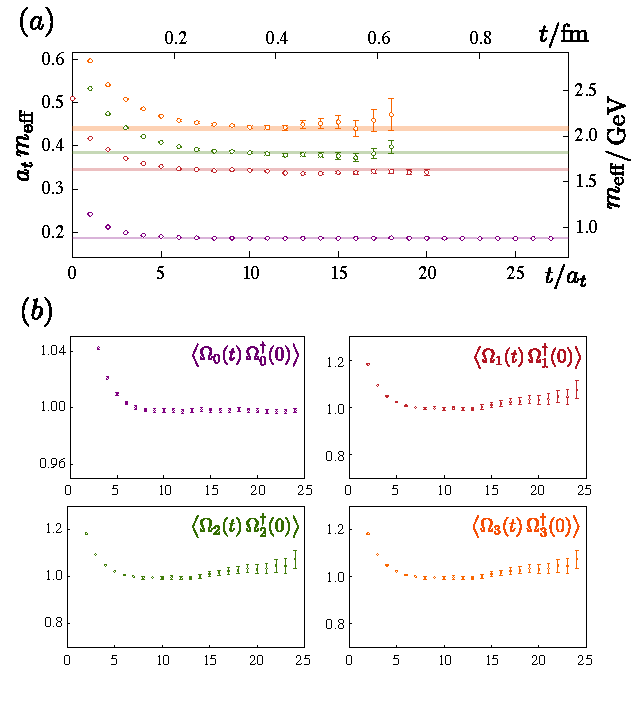
\includegraphics[width=0.8\linewidth]{figures/radTrans/PrinCorr_Eff_D4A2M_mom1.pdf}
\caption{(a) Effective masses of principal correlators for four lightest states in the $A_2^+$ irrep for momentum direction $\vec{n}_{\vec{p}} = [1,0,0]$ along with the energy determined from a two exponential fit. (b) `Optimized' operator correlation functions, $(2E_\mathfrak{n})^{-1} e^{E_\mathfrak{n}t} \big\langle \Omega_\mathfrak{n}(t) \, \Omega_\mathfrak{n}^\dag(0) \big\rangle$, for the four states shown above.\label{fig::SpecD4A2M}}
\end{centering}
\end{figure}
\clearpage
}

%%%%%%%%%%%%%%%%%%%%%%%%%%%%%%%%%%%%%%%%%%%%%%%%%%%%%%%%%
%%%%%%%%%%%%%%%%%%%%%%%%%%%%%%%%%%%%%%%%%%%%%%%%%%%%%%%%%
%%%%%%%%%%%%%%%%%%%%%%%%%%%%%%%%%%%%%%%%%%%%%%%%%%%%%%%%%

\subsection{Three-Point Functions Using Optimized Operators} \label{sec::OptOps}
Turning first to the case of three-point functions with pion-like operators at the source and sink, we plot in \figref{fig::ThreePointRelaxationPion} the form-factor (as defined in \eqnref{eqn::pion_decomp}) extracted from the three-point function, 
\begin{equation*}
\langle 0 | \mathcal{O}_\pi(\Delta t,\vec{p}_f) j^\mu(t, \vec{q}) \mathcal{O}^\dagger_\pi(0,\vec{p}_i) | 0 \rangle
\end{equation*}
where $\mathcal{O}_\pi$ represents either $\bar{\psi}\gamma_5\psi$ (in red) or the optimized operator $\Omega_\pi$ (in blue). The sink operator, located at $\Delta t = 28\, a_t \sim 0.9 \;\mathrm{fm}$, is in the $\Lambda^C = A_2^+$ irrep of momentum $\vec{n}_{\vec{p}_f} = [1,0,0]$, while the source operator, located at $t = 0$, is at rest in the $\Lambda^{PC} = A_1^{-+}$ irrep. We clearly observe that the optimized operators give rise to a signal which is flat over a number of timeslices away from the source and sink, corresponding to the contribution of just the ground-state pion, while the simpler $\bar{\psi}\gamma_5\psi$ operators over this time range always retain a non-negligible pollution from excited states. Such behavior is expected from our two-point function analysis: for example, at rest we find $\left| \tfrac{ \langle 0 | \bar{\psi}\gamma_5 \psi | \mathfrak{n} = 1\rangle}{  \langle 0 | \bar{\psi}\gamma_5 \psi | \mathfrak{n} = 0\rangle} \right| \sim 0.73$, so the distillation smeared operator $\left[ \bar{\psi} \gamma_5 \psi \right]^\dagger $, acting on the vacuum, creates both the ground and first excited state with comparable strength.

Our principal motivation for using optimized operators is to get access to transitions involving excited states. \figref{rhopiproj} we show matrix elements extracted from three-point correlation functions computed using either the ground-state $\pi$ or first-excited state $\pi'$ optimized operator at the source ($t_i=0,\, \vec{p}_i=[\text{-}1, 0, \text{-}1]$) and either the ground-state $\rho$ or first-excited state $\rho'$ operator at the sink ($t_f = 20\,a_t,\, \vec{p}_f=[1, 0, \text{-}1]$). We observe that there are clear statistically significant signals for excited-state transitions when using the appropriate optimized operators.

%%%%%%%%%%%% OPTIMIZED VERSUS STANDARD OPS %%%%%%%%%%%%%%%%%%%%
\afterpage{
\begin{figure}[htbp]
\begin{centering}
\includegraphics[width=0.8\linewidth]{figures/radTrans/ThreePointRelaxationPion.pdf}
\caption{Form-factor from vector current three-point function with pion operators at source ($t=0$, $\vec{n}=[0,0,0]$) and sink ($\Delta t = 28\,a_t$, $\vec{n} = [1,0,0]$). Red points correspond to using the `unoptimized' bilinear $\bar{\psi} \gamma_5 \psi$;  the `optimized' operator is shown in blue. \label{fig::ThreePointRelaxationPion}}
\end{centering}
\end{figure}
\clearpage
}

%%%%%%%%%%%% OPTIMIZED GROUND STATES & EXCITED %%%%%%%%%%%%%%%%%%%%
\afterpage{
\begin{figure}[htbp]
\begin{centering}
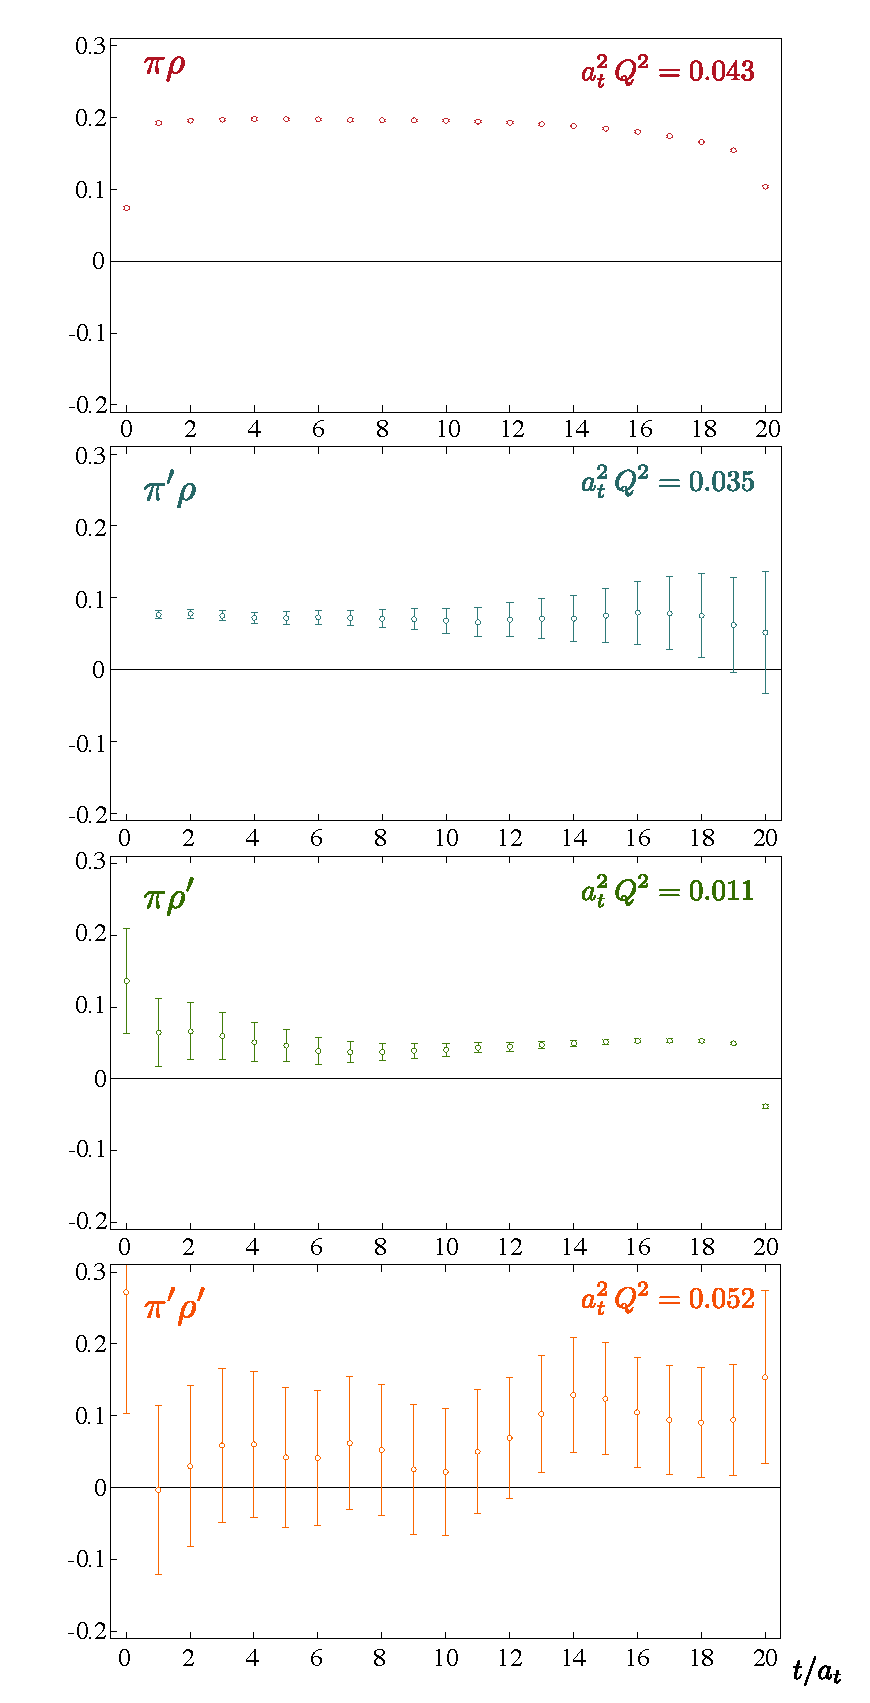
\includegraphics[width=0.5\linewidth]{figures/radTrans/ThreePointProjection.pdf}
\caption{ Form-factors extracted from optimized three-point correlation functions with a $\pi$ or $\pi'$ operator with ${\vec{p}=[\text{-}1,0,\text{-}1]}$ at $t=0$ and a $\rho$ or $\rho'$ operator with ${\vec{p}=[1,0,\text{-}1]}$ at $t= 20\,a_t$. The source-sink separation in physical units is roughly 
0.7 fm. \label{rhopiproj}}\end{centering}
\end{figure}
\clearpage
}

%%%%%%%%%%%% DEPENDENCE ON DELTA-T AND FITTING %%%%%%%%%%%%%%%%%%%%
\afterpage{
\begin{figure}[htbp]
\begin{centering}
\includegraphics[width=\linewidth]{figures/radTrans/Fpi_src_snk_separation_combined.pdf}
\caption{ Upper panel shows the pion ground-state form-factor extracted from correlation functions with source-sink separations of $\Delta t = (12,16,28)\, a_t$ using the procedure of fitting with \eqnref{three_point_fit}. The lower panel illustrates this using the example of $\vec{n}_{\vec{p}_i} = [1,0,0],\, \vec{n}_{\vec{p}_f} = [2,0,0]$.\label{fig::ThreePointSourceSinkSeparation}  }
\end{centering}
\end{figure}
\clearpage
}

In general, even for optimized operators, there may still be some residual contamination coming from states that lie beyond the reach of our variational basis, and indeed curvature away from flat behavior as we approach the source or sink timeslice is observed in Figures~\ref{fig::ThreePointRelaxationPion} and \ref{rhopiproj}. 

In order to make maximal use of the time-series data, in particular in those regions where there remains some unwanted excited-state contribution, we opt to perform a correlated fit over a time range with the form,
\begin{equation}
F(Q^2; t) =  F(Q^2)  + f_f \, e^{-\delta E_{f}\,(\Delta t - t)} + f_{i} \,  e^{- \delta E_i\, t} 
\label{three_point_fit}
\end{equation}
where $f_f, \delta E_f, f_i, \delta E_i$ and $F(Q^2)$ are real fit parameters. We make further use only of the constant term, which corresponds to the desired form-factor. Fitting the data to this form also exposes the energy scale of the pollution terms, $\delta E_f$ and $\delta E_i$. Generically, when present, we find that these energies lie at or above the scale of the largest energies we reliably extract in our two-point function variational analysis. In cases where there is a clear extended plateau region, we may exclude the exponential terms and perform a fit to a constant value.


We demonstrate the viability of our fitting method in \figref{fig::ThreePointSourceSinkSeparation}. A visible plateau is only observed for $\Delta t = 28\, a_t$, while for $\Delta t = 12\, a_t, 16\, a_t$, we make use of a fit using \eqnref{three_point_fit}, extracting compatible values for the form factor even in the face of significant amounts of pollution. The upper panel shows that this procedure is generally applicable and leads to form-factors from each time-separation that are in agreement across a range of $Q^2$ -- additional values of $\Delta t$ were also explored with similar results.

In practice, while we extract a very large number of form-factor determinations at many $Q^2$-values, we choose to make use of only those where application of \eqnref{three_point_fit} to $F(Q^2;t)$ shows modest excited-state contributions. Any cases where a clear trend toward a constant value is not visible are discarded.

%%%%%%%%%%%%%%%%%%%%%%%%%%%%%%%%%%%%%%%%%%%%%%%%%%%%%%%%%
%%%%%%%%%%%%%%%%%%%%%%%%%%%%%%%%%%%%%%%%%%%%%%%%%%%%%%%%%
%%%%%%%%%%%%%%%%%%%%%%%%%%%%%%%%%%%%%%%%%%%%%%%%%%%%%%%%%

\subsection{Extracting Form Factors} \label{sec::FFExtract}
In \eqnref{eqn::genericDecompositionHelicity} we present the most general form of the decomposition of a vector current matrix element into independent form factors, $F_i(Q^2)$, multiplying their associated kinematic factors, $K_i^\mu$, which are functions of the momentum, spin, and helicity projection. Moving, for the moment, to an exhaustive notation, we see that we can decompose a three-point correlation function featuring \emph{optimized} operators as 
\begin{align}
\langle 0 | \Omega_{\estate{n}_f,\vec{p}_f, \lambda_f}(\Delta t) &j^\mu_{\vec{q}}(t) \Omega^\dagger_{\estate{n}_i,\vec{p}_i, \lambda_i}(0) | 0 \rangle \notag \\ &= e^{-E_{\estate{n}_f}(\Delta t - t)} e^{-E_{\estate{n}_i}t} \langle \estate{n}_f ,\vec{p}_f, \lambda_f | j^\mu | \estate{n}_i,\vec{p}_i, \lambda_i \rangle + \ldots \label{eqn::llsq_p}\\ 
&=  e^{-E_{\estate{n}_f}(\Delta t - t)} e^{-E_{\estate{n}_i}t} \sum_j K^\mu_j(\estate{n}_f ,\vec{p}_f, \lambda_f;\estate{n}_i,\vec{p}_i, \lambda_i ) F_j(Q^2) + \ldots \notag,
\end{align}
where the ellipses represent suppressed contributions from states other than ($|\estate{n}_f\rangle , |\estate{n}_i\rangle $), which have been shown in the preceding subsection to be small. 

In general \eqnref{eqn::llsq_p} represents an under-determined linear system. This is to say that on the l.h.s. we have a single matrix element while on the right there are multiple form factors appearing which must be disentangled. We choose to build a constrained or over-constrained linear system featuring many such equations, each occurring at the same $Q^2$, which we then invert to obtain the form factors, $F_j(Q^2)$. Fixing the state choices, $\estate{n}_{f,i}$, using the indexing $a = \left(\vec{p}_f, \lambda_f;\mu;\vec{p}_i \lambda_i\right)$, and removing the time dependence we can rewrite the above equation as 
\begin{align}
\Gamma_a(\Delta t, t) &= e^{E_{\estate{n}_f}(\Delta t - t)} e^{E_{\estate{n}_i}t} \langle 0 | \Omega_{\estate{n}_f,\vec{p}_f, \lambda_f}(\Delta t) j^\mu_{\vec{q}}(t) \Omega^\dagger_{\estate{n}_i,\vec{p}_i, \lambda_i}(0) | 0 \rangle \notag \\
&= \sum_jK_j(a)F_j(Q^2) + \ldots.
\end{align}
In this manner we exploit the redundancy of form factors appearing for different current components and helicity combinations. We also, in some cases, average over kinematically equivalent momenta. 

The linear system we solve is $\mathbb{\Gamma} = \mathbb{K} \cdot \mathbb{F}$. Here $\mathbb{\Gamma}$ is a vector over the index $a$, each element $\Gamma_a(\Delta t,t)$, $\mathbb{K}$ a matrix over kinematic factors with indices $a$ and $j$, and $\mathbb{F}$ a vector of form factors indexed by $j$.  A general formulation of such a linear system need not be square, indeed in practice we build over-constrained rectangular linear systems. The system can be converted into a square system: $\mathbb{K}^\dagger \mathbb{\Gamma} = \left[ \mathbb{K}^\dagger \mathbb{K} \right ] \mathbb{F}$, which we invert using SVD\footnote{In the case where only a single form factor contributes this method of solution reduces to computing an average.}. 


%%%%%%%%%%%%%%%%%%%%%%%%%%%%%%%%%%%%%%%%%%%%%%%%%%%%%%%%%
%%%%%%%%%%%%%%%%%%%%%%%%%%%%%%%%%%%%%%%%%%%%%%%%%%%%%%%%%
%%%%%%%%%%%%%%%%%%%%%%%%%%%%%%%%%%%%%%%%%%%%%%%%%%%%%%%%%

\subsection{Cubic Symmetry} \label{sec::CubSym}
Implicit in the previous sections were a number of assumptions about the nature of states we see in our lattice calculation. Specifically we took advantage of Lorentz symmetry (by assuming we could relate various components of the current to one another) and the organization of hadrons into irreducible representations of the continuous rotation group labeled by an integer $J$ (in the construction of kinematic decompositions) -- neither of these are explicitly good symmetries on the lattice.  

The \emph{cubic} grid, on which we run simulations, is only invariant under cubic rotations, a subset of all rotations, and as such there are different irreps (as discussed in \secref{Spec::Subduce}). To correctly reflect the symmetry of our theory then, we should label our correlation functions according to irreducible representations of the cubic symmetry. In practice this is what we do by computing using the subduced operators introduced in \secref{sec::OptOps}. Using these operators, the three-point functions take the form,
\begin{equation}
	\big\langle 0 \big| \Omega_{\mathfrak{n}_\mathrm{f}, \vec{p}_\mathrm{f}}^{\Lambda_\mathrm{f},\mu_\mathrm{f}}(\Delta t) \, j_{\vec{q}}^{\Lambda_\gamma, \mu_\gamma}(t) \, \Omega_{\mathfrak{n}_\mathrm{i}, \vec{p}_\mathrm{i}}^{\Lambda_\mathrm{i},\mu_\mathrm{i}\dag}(0) \big| 0 \big\rangle, \label{subduced_3pt}
\end{equation}
where the indices $\Lambda$, $\mu$ label the cubic group irrep and the `row' ($1\cdots\text{dim}(\Lambda)$) of the irrep. 

As explained in \secref{Spec::Cubic} it \emph{may} be the case that there are underlying continuum-like symmetries which emerge when the mesh becomes sufficiently fine.  It would be irresponsible to use this putative symmetry without first demonstrating its realization in explicit calculation\footnote{The linear system, as presented, would also not be satisfactorily solvable if the symmetry were not present.}. 

\afterpage{
\begin{sidewaysfigure}[htbp]
\begin{center}
\includegraphics[width=\linewidth]{figures/radTrans/RotationalSymmetryRestoration.pdf}
\end{center}
\caption{Left: We plot the mass spectrum for the lowest $J^{PC} = 1^{--}, 1^{+-}$ states projected onto momentum $\vec{n}_{\vec{p}} = [110]$ across the $\Lambda^C = A_1^-,B_1^-,B_2^-,A_2^-$ little group irreps observing degeneracy patterns corresponding to the $\rho$ and $b_1$ mesons. Right: Transition form-factors extracted from the three point function $\langle 0 | \Omega_\rho(28,\vec{p}\;') j^\mu(t,\vec{q}) \Omega_\pi^\dagger(0,\vec{p}) | 0 \rangle$ with  $\vec{n}_{\vec{p}\;'} = [0,1,1]$, $\vec{n}_{\vec{p}} = [0,\text{-1},1]$, and $\vec{n}_{\vec{q}}  = [0,2,0]$.  Observation of consistent form-factor values indicates that we are resolving the different helicity components of a $1^{--}$ meson.  \label{fig::RotSymRest}}
\end{sidewaysfigure}
\clearpage
}

As a primer we first consider the left panel of \figref{fig::RotSymRest} where we show an example of the extracted spectrum across little-group irreps, $\Lambda^C = A_1^-, B_1^-, B_2^-, A_2^-$ for $n_{\vec{p}}=[110]$, where the distribution of states matches the expected subduction patterns for two meson states, a lighter $\rho$ ($J^{PC}=1^{--}$) state and a heavier $b_1$ ($J^{PC}=1^{+-}$) state.

In order to investigate if the lower pattern really does correspond to the different helicity projections of a $J^{PC} =1^{--}$ state we form the optimized `$\rho$' operator  in each of the $A_1^-, B_1^-, B_2^-$ irreps. We then compute the three-point function, 
\begin{equation*}
\langle 0 | \Omega_\rho(\Delta t,\vec{p}\,')\,  j^\mu(t,\vec{q}\,) \,  \Omega_\pi^\dagger(0,\vec{p}\,) | 0 \rangle,
\end{equation*}
for $\vec{n}_{\vec{p}\,'} = [0,1,1]$, $\vec{n}_{\vec{p}} = [0,\text{-}1,1]$, and $\vec{n}_{\vec{q}} = [0,2,0]$. The source operator is the optimized operator for the ground-state pion in the $A_2^+$ irrep. The three different sink irrep choices correspond to the subduced versions of the three helicity projections of a vector meson. For $\Delta t = 28\,  a_t$, the resulting form-factor is plotted in \figref{fig::RotSymRest}, where we observe that while the amount of excited state pollution differs slightly in each irrep, the form-factor values are consistent, indicating that we are observing components of the same $1^{--}$ meson in the three irreps. 

We expect to see a comparable restoration of the rotational symmetry across this calculation, we do not attempt to build decompositions according to the symmetries of the cube, rather making use of the continuum-like helicity decompositions presented earlier, subduced trivially into irreducible representations of the cube. 

A slight additional complication in this analysis arises from our use of anisotropic gauge configurations in which the space and time directions are discretized with different spacings. Spatially directed currents will need to be renormalized separately from temporal currents and the discretization effects along the two directions are expected to be different -- in explicit calculation we will not mix spatially directed currents with their temporal counterparts. Had we used isotropic lattices the temporal component of the vector current would be related to the spatial components, however here we will keep them separate with the temporal component of the current subducing differently from the spatial components. For spatial components, the subduced current is $j_{\vec{q}}^{\Lambda_\gamma, \mu_\gamma} = \sum_\lambda \mathcal{S}^{\Lambda_\gamma, \mu_\gamma}_{J=1,\lambda} \, j^\lambda$ where $j^\lambda = \vec{\epsilon}(\vec{q}, \lambda) \cdot \vec{j}$, whereas temporal components subduce as $j_{\vec{q}}^{\Lambda_\gamma, \mu_\gamma} = \mathcal{S}^{\Lambda_\gamma, \mu_\gamma}_{J=0} \, j^{\nu=0}$. 

In order to relate the irrep-based correlation functions that we compute, \eqnref{subduced_3pt}, to the helicity-based decompositions presented in \eqnref{eqn::genericDecompositionHelicity}, we define subduced matrix elements, which for the spatial current case take the form,
\begin{align}
\big\langle  \mathfrak{n}_\mathrm{f}, &\vec{p}_\mathrm{f}, \Lambda_\mathrm{f}, \mu_\mathrm{f} \big| j^{\Lambda_\gamma, \mu_\gamma} \big| \mathfrak{n}_\mathrm{i}, \vec{p}_\mathrm{i}, \Lambda_\mathrm{i}, \mu_\mathrm{i} \big\rangle  \nonumber \\
	= &\sum_{\lambda_\mathrm{f}, \lambda_\gamma, \lambda_\mathrm{i}} S^{\Lambda_f, \mu_f}_{J_f,\lambda_f}  S^{\Lambda_\gamma ,\mu_\gamma}_{J_\gamma =1 ,\lambda_\gamma}  \left[S^{\Lambda_i ,\mu_i}_{J_i,\lambda_i}\right]^*  \sum\nolimits_l \, \vec{\epsilon}(\vec{q},\lambda_\gamma) \cdot \vec{K}_l\big(h_{f,J_f}\big(\lambda_f,\vec{p}_f); h_{i,J_i}(\lambda_i,\vec{p}_i) \big) \, F_l(Q^2).  \label{eqn::subduced_decomp}
\end{align}
%\footnote{The use of the Lorentz-covariant decomposition in this expression implies relationships between different irreps that we must establish are present in the computed correlation functions for this approach to be considered reasonable.}

%%%%%%%%%%%%%%%%%%%%%%%%%%%%%%%%%%%%%%%%%%%%%%%%%%%%%%%%%
%%%%%%%%%%%%%%%%%%%%%%%%%%%%%%%%%%%%%%%%%%%%%%%%%%%%%%%%%

\subsection{Renormalization} \label{sec::Renormalization}
In our calculation we use a local vector current, $\bar{\psi}\gamma^\mu\psi$ which is not conserved at finite lattice spacing and must be renormalized, multiplicatively, by a factor $Z_V$. Further, owing to our anisotropic formulation, in which we discretize space and time differently, there can be one $Z_V$ for the spatially directed current, $\bar{\psi} \gamma^i\psi$, and another for the temporal direction, $\bar{\psi}\gamma^0\psi$.   

The renormalization coefficient can be determined non-perturbatively via computing the charge form factor of $\pi^+$ or $\rho^+$ at zero momentum transfer ($Q^2 = 0$). In the continuum this corresponds to a measurement of the total charge of the meson in units of $e$, the elementary charge ($F(0)=1$). We define the coefficient as 
\begin{equation}
Z_V = \frac{F^{\mathrm{cont.}}(0)}{F^{\mathrm{lat.}}(0)} = \frac{1}{F^{\mathrm{lat.}}(0)}. 
\end{equation}

The value is extracted from correlation functions of the form 
\begin{equation*}
\langle 0 | \Omega_\pi(\Delta t, \vec{p})  j^\mu(t,\vec{q}=\vec{0}) \Omega_\pi^\dagger(0,\vec{p}) | 0 \rangle.
\end{equation*}
 We plot the results, as a function of momentum, for the $\pi^+$ and $\rho^+$ mesons in \figref{fig::Z_V}. The dependence on momentum appears to be fairly mild, each value being consistent with the others. There is however dependence on particle type -- renormalization factors extracted from the rho meson differ from those extracted from the pion in a statistically significant manner. This can perhaps be attributed to discretization effects which may appear differently for the two particles\footnote{Some small amount of the discrepancy may also arise from an imperfect tuning of the action -- in a simple sense we tune the anisotropy in both the gauge and the fermion action, a slight mismatch of these parameters may give rise to additional effects beyond the scope of this analysis.} as well as the fact that we have not used a conserved vector current\footnote{If we had used a conserved current we would not need to renormalize the current.}.

\afterpage{
\begin{figure}[htbp]
\begin{center}
\includegraphics[width=\linewidth]{figures/radTrans/Z_V.pdf}
\end{center}
\caption{Vector current renormalization factor extracted at $Q^2=0$ from the pion (circles) and the rho (squares). Spatially directed currents appear in blue and green, temporal in red and orange. \label{fig::Z_V}}
\end{figure}
\clearpage
}

We set the scale of the charge via the pion extraction as it is statistically the most precise. The data are fit, including data covariance, to obtain 
\begin{equation}
	Z_V^s = 1.180(4), \;\; Z_V^t = 1.037(4),
\end{equation}
for the spatial and temporal renormalization factors respectively. All subsequent presentations of form-factor values in this paper have been multiplicatively renormalized by these factors.









\chapter{Results}

\section{calculation details} \label{sec::res::calc_det}

In this first investigation of the extraction of excited state form-factors using distillation, we restrict ourselves to a single ensemble of gauge-field configurations, having three degenerate flavors of dynamical quarks tuned to approximately the physical strange quark mass. This set of anisotropic Clover\footnote{Some details, including a brief derivation of the action may be found in \appref{app::Clover}.} lattices \cite{Edwards:2008ja, Lin:2008pr} has been used previously in studies of the meson spectrum \cite{Dudek:2009qf,Dudek:2010wm,Dudek:2011tt,Liu:2012ze,Dudek:2013yja}, meson decay constants~\cite{Mastropas:2014fsa}, baryon spectrum \cite{Edwards:2011jj, Dudek:2012ag, Edwards:2012fx, Padmanath:2013zfa} and meson-meson scattering \cite{Dudek:2010ew,Dudek:2012gj,Dudek:2012xn,Dudek:2014qha}. For the calculations reported on in this paper, we used 535 configurations of lattice volume $(L/a_s)^3 \times (T/a_t) = 16^3\times 128$, with a spatial grid spacing of $a_s \sim 0.12\, \mathrm{fm}$ and a temporal spacing roughly 3.5 times smaller. 

In this calculation we have an exact $SU(3)$ flavor symmetry such that all the octet mesons ($\pi$, $K$, $\eta$) are degenerate with a mass close to $700$ MeV. Where results are expressed in dimensionful units, they are determined from the dimensionless quantities $a_t E$ using the scale-setting procedure,
\begin{equation*}
E = \frac{a_t E}{a_t m_\Omega} \cdot m_\Omega^{\mathrm{phys.}}.
\end{equation*}
where $a_t m_\Omega$ is the $\Omega$ baryon mass calculated on this lattice and $m_\Omega^{\mathrm{phys.}}$ is the experimental value \cite{PDG-2012}.



\section{Extracted form-factors \& transitions\label{sec::results}}

In this section we present form-factors and transitions for the lightest few isovector pseudoscalar and vector mesons. We make use of the current ${  j^\nu = +\frac{2}{3}\bar{u}\gamma^\nu u -\frac{1}{3}\bar{d}\gamma^\nu d -\frac{1}{3}\bar{s}\gamma^\nu s  }$, such that the form-factors are in units of $e$, the magnitude of the electron charge. This calculation is performed with three flavors of dynamical quark all having the same mass, tuned approximately to the physical strange quark mass. We extract vector current matrix elements between ${(I,I_z) = (1,+1)}$ members of $SU(3)_F$ octets. Disconnected diagrams do not contribute to the amplitudes considered in this analysis as demonstrated in the appendix of \cite{Shultz:2015pfa}, where the flavor structure of the current is explored further.


%%%%%%%%%%%%%%%%%%%%%%%%%%%%%%%%%%%%%%%%%%%%%%%%%
%%% FORM-FACTORS
%%%%%%%%%%%%%%%%%%%%%%%%%%%%%%%%%%%%%%%%%%%%%%%%%

\subsection{Form-factors}


\subsubsection{$\pi$ form-factor}

The pion form-factor appears in the matrix element decomposition, $\big\langle \pi^+(\vec{p}\,') \big| j^\mu \big| \pi^+(\vec{p}) \big\rangle = (p+p')^\mu \, F_\pi(Q^2)$, which we will extract from three-point Euclidean correlation functions computed using optimized ground-state pion operators of definite momentum at the source (at $t=0$) and the sink (at $\Delta t = 28\, a_t$). As discussed previously, we will present $F(Q^2;t)$, where the leading Euclidean time-dependence of the correlation function has been removed, with any remaining time-dependence signaling the presence of excited state contributions to the correlation function. By utilizing many values of $\vec{p}$ and  $\vec{p}\,'$ we can determine the form-factor at a range of $Q^2$ values. We plot $F_\pi(Q^2;t)$ for a subset of these $Q^2$ values in Figure~\ref{fig::pion_proj0_pion_proj0_Q2_dep}, where for each $Q^2$ we overlay a fit according to the form in \eqnref{three_point_fit}.

\afterpage{
\begin{figure}[htbp]
\begin{centering}
  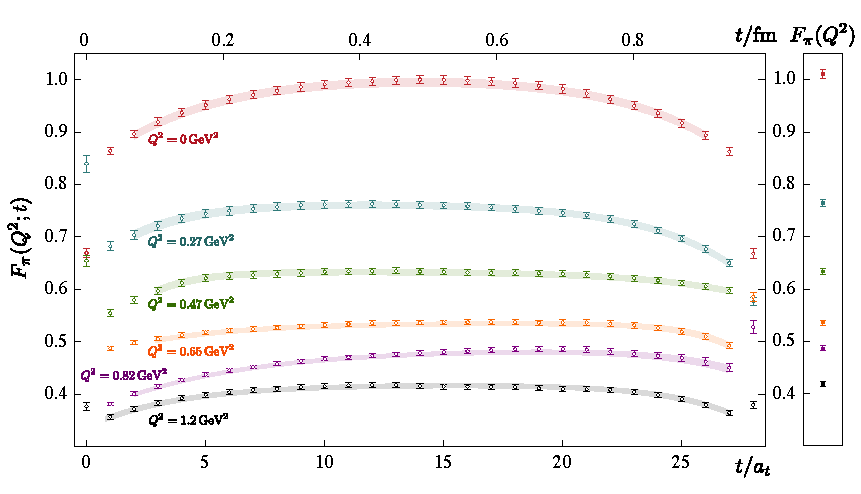
\includegraphics[width=0.8\linewidth]{figures/radTrans/pion_proj0_pion_proj0_Q2_dep.pdf}
  \caption{ Typical $F_\pi(Q^2; t)$ extracted from optimized three-point functions (points) with fit descriptions using \eqnref{three_point_fit} (curves). Note that the data points have a high degree of timeslice correlation which is accounted for in the fitting.  \label{fig::pion_proj0_pion_proj0_Q2_dep}}
    \end{centering}
\end{figure}
\clearpage
}

\afterpage{
\begin{figure}[htbp]
\begin{centering}
  \includegraphics[width=0.8\linewidth]{figures/radTrans/pion_proj0_pion_proj0.pdf}
  \caption{ Pion ground-state form-factor, $F_\pi(Q^2)$, using the improved current, see \secref{app::Clover}. Vector meson dominance using the $\rho$ meson mass on this lattice shown by the dashed curve. Fits to the small-$Q^2$ points using gaussian and single-pole forms shown by the gray curves. \label{fig::pion_formfactor} }
    \end{centering}
\end{figure}
\clearpage
}


In Figure~\ref{fig::pion_formfactor} we plot the resulting $Q^2$ dependence, shown via both dimensionless $a_t^2 Q^2$ and scale-set using the $\Omega$-baryon mass prescription presented in \secref{sec::res::calc_det}. A large number of kinematic points are sampled by considering all combinations of momentum such that $n^2_{\vec{p}} \le 4$, $ n^2_{\vec{p}\,'} \le 4$ and $ n^2_{\vec{q}} \le 4$. The extracted points appear to lie on a single curve, with only small residual scatter which can originate from fitting-range systematics and modest discretization effects.

Describing the $Q^2$ dependence may offer some phenomenological insight, albeit in this calculation at an unphysically heavy quark mass. A commonly used approach to describe vector-current form-factors of hadrons is to argue that the photon is behaving like the lightest vector meson which can couple to the hadrons in question, which in this case would be the $\rho$. This ``vector meson dominance"(VMD) describes the $Q^2$ dependence by ${F_{\mathrm{VMD}}(Q^2) = \frac{1}{1 + Q^2/m_\rho^2 }}$. Using the $\rho$ mass determined on these lattices, $m_\rho = 1020(1)\, \mathrm{MeV}$, we have the dashed curve shown in Figure~\ref{fig::pion_formfactor}, which is seen to describe the lattice data reasonably well only for small photon virtualities. One possible explanation of this effect is that as we move out to larger $Q^2$, considering only the nearest time-like pole, the $\rho$, and neglecting all excitations, becomes a progressively poorer approximation.

 
The distribution of charge within the pion can be characterized by the \emph{charge radius}, defined via the slope of the form-factor at zero virtuality, ${\langle r^2 \rangle \equiv -6 \frac{d}{dQ^2}F(Q^2) \big|_{Q^2=0}}$. We may obtain this quantity from the discrete $Q^2$ data presented in Figure~\ref{fig::pion_formfactor} by parameterizing the $Q^2$--dependence for small virtualities. Considering gaussian ${ \big(  F_\pi(Q^2) = F(0)\, e^{-Q^2/16\beta^2}  \big) }$ and pole ${ \big(  F_\pi(Q^2) = F(0)\, \tfrac{1}{1 + Q^2/m^2} \big) }$ forms to describe ${Q^2 < 0.3\,\mathrm{GeV}^2}$, we obtain\footnote{If $F(0)$ is allowed to float in fits, a value statistically compatible with 1 is obtained, as it must since the pion form-factor at zero $Q^2$ was used to set $Z_V$. The fit $\chi^2$ values obtained are fairly large due to the scatter in the statistically precise data, which is likely due to small discretization effects which are not described by these smooth fit-forms.} 
a charge radius ${  \langle r^2 \rangle_{\pi}^{1/2} = 0.47(6) \; \mathrm{fm}  }$, where the error includes the variation over fit-form. As we might expect, in a calculation where three flavors of quarks all have approximately the strange quark mass, we obtain a pion charge radius somewhat smaller than the physical pion ${\langle r^2 \rangle_\pi^{1/2} = 0.67(1)\,\mathrm{fm}}$ \cite{Amendolia:1986wj, PDG-2012}, and also smaller than the physical kaon ${  \langle r^2 \rangle_K^{1/2} = 0.58(4) \, \mathrm{fm}  }$ \cite{Amendolia:1986ui}.








%%%%%%%%%%%%%%%%%%%%%%%%%%%%%%%%%%%%%%%%%%%%%%%%%%%%%%%%%%%%%%%%%%%%%%%%%%%%%%%%%%%%%%%%%%%
%%%%%%%%%%%%%%%%%%%%%%%%%%%%%%%%%%%%%%%%%%%%%%%%%%%%%%%%%%%%%%%%%%%%%%%%%%%%%%%%%%%%%%%%%%%
\subsubsection{$\rho$ form-factors}



The three form-factors required to describe the vector-current response of a vector hadron may be defined as in \eqnref{eqn::rho_Gmultipole_basis}, which makes use of a multipole basis. The decomposition presented in \eqnref{eqn::rho_Gi_basis} defines the linear system which we may solve, as described in \secref{sec::FFExtract}, for the form-factors. We plot the charge, $G_E(Q^2)$, magnetic, $G_M(Q^2)$, and quadrupole, $G_Q(Q^2)$ form-factors in Figure~\ref{fig::rho_form_factors}. Examination of Equations~\ref{eqn::rho_Gi_basis}, \ref{eqn::rho_Gmultipole_basis} indicates that only the charge form-factor has a non-zero kinematic factor when $Q^2=0$, and as such only it is determined there, while all three form-factors are sampled for positive non-zero $Q^2$. The smallest form-factor, $G_Q$, shows the largest scatter, which likely originates from modest discretization effects and timeslice fitting-range fluctuations.

\afterpage{
\begin{figure}[htbp]
\begin{centering}
  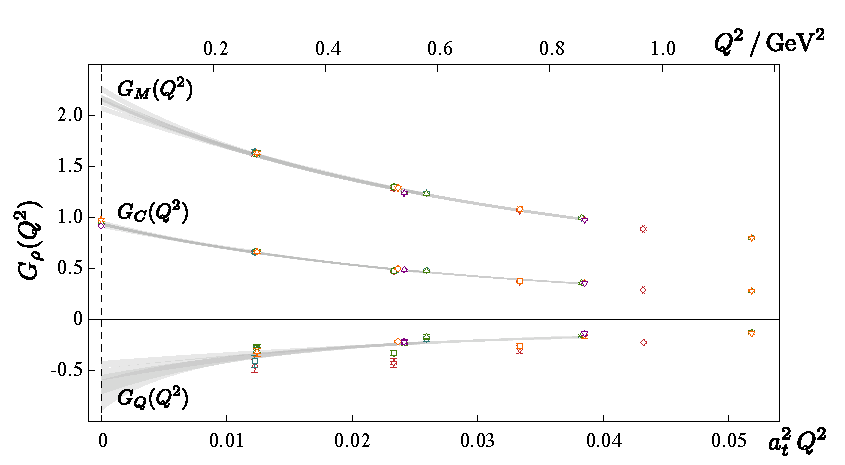
\includegraphics[width=0.80\linewidth]{figures/radTrans/rho0_rho0.pdf}
  \caption{ Ground-state $\rho$ meson multipole form-factors. Points have the same color and shape labeling presented in Figure~\ref{fig::pion_formfactor}. Fits to the $Q^2$ dependence, described in the text, are shown as gray curves. \label{fig::rho_form_factors}}
    \end{centering}
\end{figure}
\clearpage
}


Fitting the $Q^2$ dependence of the charge form-factor with various forms\footnote{$G(0) e^{-Q^2/16\beta^2}$, $G(0) e^{-Q^2(1+\alpha Q^2)/16\beta^2}$, $G(0)/(1+ Q^2/m^2)$, $G(0)/(1+ Q^2/m^2 + \gamma (Q^2/m^2)^2 )$, $G(0) \frac{e^{-Q^2/16\beta^2}  }{1+Q^2/m^2}$ }, over various $Q^2$ ranges we obtain $G_C(0) = 0.94(1)$ and ${  \langle r^2 \rangle_\rho^{1/2} = 0.55(5) \, \mathrm{fm} }$ where the errors include a systematic variation over different fit forms. The deviation of the charge from 1 was discussed previously \secref{sec::Renormalization}. 

In order to determine the magnetic and quadrupole moments from $G_M(0)$ and $G_Q(0)$ it is necessary to parameterize the $Q^2$ dependence of the form-factors and extrapolate back to $Q^2=0$. Utilizing a range of possible forms, we obtain ${G_M(0) = 2.17(10)}$ and ${G_Q(0) = -0.54(10)}$, accounting for the variation over fit-forms, which is much larger than the statistical uncertainty, in the errors. More precise determinations of these quantities could be obtained if twisted boundary conditions were used to sample the form-factors at smaller $Q^2$ (see for example \cite{Flynn:2005in}).

Within a simple picture of the $\rho$ as a $q\bar{q}$ bound-state, the presence of a quadrupole moment would indicate a required admixture of $D$-wave into the dominantly $S$-wave wavefunction. Previous estimates of the $\rho$-meson magnetic moment in versions of QCD with heavier than physical quarks come from chiral effective theory \cite{Djukanovic:2013mka} where $G_M(0) \sim 2.2$ for large pion masses, and quenched lattice QCD using either an energy shift in a magnetic field \cite{Lee:2008qf} where $G_M(0) = 2.13(6)$, or extrapolation to zero $Q^2$ from a single spacelike virtuality \cite{Hedditch:2007ex} where $G_M(0) = 2.05(4)$, at comparable unphysical pion masses. A dynamical calculation, Ref.~\cite{Owen:2015gva}, which appeared while this manuscript was in the final stages of production, found, at a comparable pion mass, $G_M(0) = 2.23(2)$ and $G_Q(0) = -0.362(20)$, using a model extrapolation to $Q^2=0$ from a single non-zero $Q^2$ point.




%%%%%%%%%%%%%%%%%%%%%%%%%%%%%%%%%%%%%%%%%%%%%%%%%%%%%%%%%%%%%%%%%%%%%%%%%%%%
%%%%%%%%%%%%%%%%%%%%%%%%%%%%%%%%%%%%%%%%%%%%%%%%%%%%%%%%%%%%%%%%%%%%%%%%%%%%
%%%%%%%%%%%%%%%%%%%%%%%%%%%%%%%%%%%%%%%%%%%%%%%%%%%%%%%%%%%%%%%%%%%%%%%%%%%%

\subsubsection{$\pi'$ form-factor}

\afterpage{
\begin{figure}[htbp]
\begin{centering}
  \includegraphics[width=0.8\linewidth]{figures/radTrans/pion_proj1_pion_proj1_Q2_dep.pdf}
  \caption{Current insertion time dependence for the form-factor of the first excitation of the pion, $F_{\pi'}(Q^2;t)$, shown for a range of source and sink momenta. The high degree of timeslice-timeslice data correlation  is manifested in the error on the fit which is not significantly reduced relative to the error on the individual data points. \label{fig::pion_proj1_pion_proj1_Q2_dep}}
    \end{centering}
\end{figure}
\clearpage
}

\afterpage{
\begin{figure}[htbp]
\begin{centering}
  \includegraphics[width=0.8\linewidth]{figures/radTrans/pion_proj1_pion_proj1.pdf}
  \caption{First-excited pion form-factor, $F_{\pi'}(Q^2)$. Points have the same color and shape labeling presented in Figure~\ref{fig::pion_formfactor}. Fits to low $Q^2$ dependence used to constrain charge-radius, as described in text, shown as gray bands.  
  \label{fig::piStar_form_factor}}
    \end{centering}
\end{figure}
\clearpage
}



The examples presented in the previous two subsections were the lightest states with the relevant quantum numbers. As such it was not strictly necessary to use optimized operators -- any suitable meson interpolators used in the three-point functions will, in the limit of large time separations, give access to the matrix elements. We will now move to the case of an excited state, the first excitation of the pion, which we access using optimized operators to eliminate the contribution of the ground-state pion.

As described in \chapref{chap::Spectroscopy}, the signals for excited states are typically noisier than those for the ground state, and as such we separate the source and sink operators by a smaller time, in this case $\Delta t = 16 \, a_t$. The decomposition for this matrix element is of the same form as the pion described previously, \eqnref{eqn::pion_decomp}. We plot the extracted form-factor, $F_{\pi'}(Q^2; t)$, as a function of the current insertion timeslice in Figure~\ref{fig::pion_proj1_pion_proj1_Q2_dep}. 



The $Q^2$ dependence of the form-factor, $F_{\pi'}(Q^2)$, is presented in Figure~\ref{fig::piStar_form_factor}. While the extracted values at $Q^2=0$ are not statistically precise, they are certainly consistent with unity. The charge radius can be extracted from the slope at $Q^2=0$ which we determine by parameterizing\footnote{Gaussian ($F_{\pi'}(0) \, e^{-Q^2/16\beta^2}$) and one-pole ($F_{\pi'}(0) / (1 + Q^2 / m^2 )$) forms were used. }
 the data for $Q^2 \lesssim 0.3\,\mathrm{GeV}^2$, yielding ${   \langle r^2 \rangle_{\pi'}^{1/2} = 0.74(6) \, \mathrm{fm} }$ where the error includes variation over parameterization form. As we might expect for a state which likely can be characterized as a radial excitation, this is significantly larger than the $0.47(6)\,\mathrm{fm}$ found for the ground-state pion at this quark mass. 
 
Ref.~\cite{Owen:2015gva}, computing at a very similar pion mass found $0.517(4)\,{\rm fm}$ for the ground-state pion charge radius, and $0.59(3)\,{\rm fm}$ for the first excitation of the pion. Their approach determines a single point on the form-factor curve at $Q^2\sim 0.16 \,\mathrm{GeV^2}$ which is used to determine the slope at $Q^2=0$ assuming monopole dependence on $Q^2$. 




%%%%%%%%%%%%%%%%%%%%%%%%%%%%%%%%%%%%%%%%%%%%%%%%%%%%%%%%%%%%%%%%%%%%%%%%%%%%%%%%%%%%%%%%%%%%%%%%%%%%%
%%%%%%%%%%%%%%%%%%%%%%%%%%%%%%%%%%%%%%%%%%%%%%%%%%%%%%%%%%%%%%%%%%%%%%%%%%%%%%%%%%%%%%%%%%%%%%%%%%%%%
%%%%%%%%%%%%%%%%%%%%%%%%%%%%%%%%%%%%%%%%%%%%%%%%%%%%%%%%%%%%%%%%%%%%%%%%%%%%%%%%%%%%%%%%%%%%%%%%%%%%%

\subsection{Radiative Transitions}



%%%%%%%%%%%%%%%%%%%%%%%%%%%%%%%%%%%%%%%%%%%%%%%%%%%%%%%%%%%%%%%%%%%%%%%%%%%%%%%%%%%%%%%%%%%%%%%%%%%%%
\subsubsection{$\pi' \rightarrow \pi \gamma$ transition}


In a transition between different pseudoscalar mesons, the decomposition of the current in terms of a form-factor $F_{\pi' \pi}(Q^2)$ is as in \eqnref{eqn::pipip_decomp}, and the form-factor must vanish at $Q^2=0$. The transition form-factor is extracted from three-point functions with $\Delta t = 20 \, a_t$, fitting the time-dependence as previously to account for any residual unwanted excited state contribution. We plot the extracted form-factor in \figref{fig::pi_pistar_transition} -- that we are now able to explore the timelike $Q^2$ region, where previously all points were spacelike, follows from the differing masses of the hadrons at source and sink, a simple example being the case where $\vec{p}\,' = \vec{p}$, so that ${Q^2 = - \big( E'(\vec{p}\,) - E(\vec{p}\,) \big)^2 < 0}$. In order to be able to trivially relate our Euclidean amplitudes to Minkowski amplitudes, we must restrict ourselves to the region where the current is not timelike enough to produce on-shell hadrons. In this calculation where the $\pi \pi$ threshold is above the $\rho$ mass, this limits us to ${  Q^2 > - m_\rho^2 \sim - 1\,\mathrm{GeV}^2  }$. In order to explore further into the timelike region, a somewhat more sophisticated approach must be followed \cite{Meyer:2011um, Feng:2014gba}.

\afterpage{
\begin{figure}[htbp]
\begin{centering}
  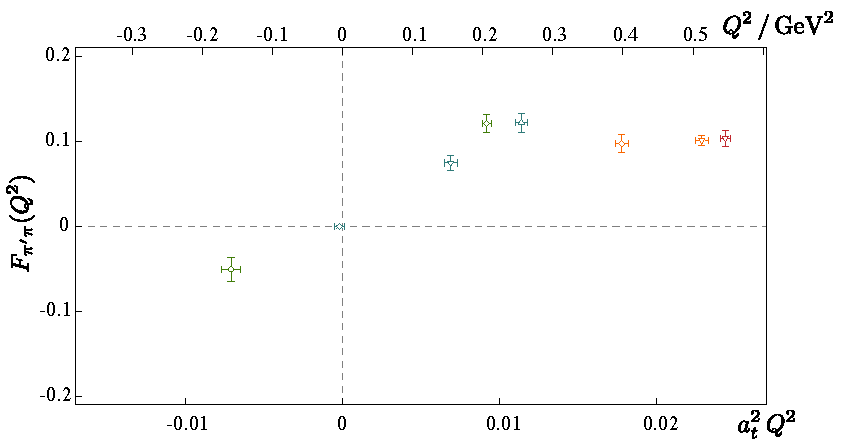
\includegraphics[width=0.8\linewidth]{figures/radTrans/pi_pistar_transition_formfactor.pdf}
  \caption{Transition form-factor between first-excited and ground-state pions, $\pi' \to \pi \gamma$. Points have the same color and shape labeling presented in Figure~\ref{fig::pion_formfactor} with the excited pion having momentum $\vec{p}_f$. \label{fig::pi_pistar_transition}}  \end{centering}
\end{figure}
\clearpage
}



%%%%%%%%%%%%%%%%%%%%%%%%%%%%%%%%%%%%%%%%%%%%%%%%%%%%%%%%%%%%%%%%%%%%%%%%%%%%%%%%%%%%%%%%%%%%%%%%%%%%%
\subsubsection{$\rho \rightarrow \pi \gamma$ transition}\label{rhopigamma}

A suitable decomposition for a vector to pseudoscalar transition in terms of a dimensionless form-factor is given in \eqnref{rho_pi_ff}. Using optimized operators for the ground-state $\rho$ and ground-state $\pi$ we computed correlation functions with $\Delta t = 28\, a_t$ for a large range of source and sink momenta -- the resulting determination of the form-factor, $F_{\rho \pi}(Q^2)$ is presented in Figure~\ref{fig::rho_pi_transition}.

The value of the form-factor at $Q^2=0$, known as the photocoupling, is of particular interest since it controls the rate of the physically allowed radiative transition process, $\rho^\pm \to \pi^\pm \gamma$. As can be seen in Figure~\ref{fig::rho_pi_transition}, we do not determine this quantity directly, but we may estimate it using interpolation between our space-like and time-like points. Using a range of fit forms over several $Q^2$ ranges (plotted in grey) we estimate $F_{\rho \pi}(0) = 0.494(8)$, where the error includes variation over fit-forms.


The Lorentz invariant matrix element for the decay $\rho^+ \to \pi^+ \gamma$ can be obtained by contracting the matrix element in \eqnref{rho_pi_ff} with a final state polarization vector, $\mathcal{M}_{\lambda_\gamma,\lambda} = \epsilon^*_\mu(\lambda_\gamma,\vec{q}) \big\langle \pi^+(\vec{p}\,') \big| j^\mu \big| \rho^+(\lambda, \vec{p}) \big\rangle$,
and for a vector stable under the strong interaction, we may obtain the decay width from
\begin{equation*}
\Gamma(\rho^+\rightarrow \pi^+\gamma) = \frac{1}{32\pi^2}\int \!\! d\Omega_{\vec{q}} \, \frac{\lvert \vec{q}\rvert}{m_\rho^2} \,  \frac{1}{3} \sum_{\lambda_\gamma,\lambda} \lvert \mathcal{M}_{\lambda_\gamma,\lambda}  \rvert^2,
\end{equation*}
where we have summed over the final state photon polarizations and averaged over the initial state polarization of the $\rho$. Using the decomposition above, and restoring the factors of $e$, we obtain the result relating the width to the photocoupling,
\begin{equation*}
\Gamma(\rho^+\rightarrow \pi^+\gamma) = \alpha\frac{4}{3} \frac{\lvert \vec{q} \rvert^3}{(m_\rho \!+\! m_\pi)^2} \lvert F_{\rho \pi}(0) \rvert^2,
\end{equation*}
where $\alpha = e^2/4\pi$. 

The calculation performed here uses three degenerate quark flavors tuned to approximate the physical strange quark mass and as such our photocoupling determination cannot be directly compared with experiment. For orientation we show in Figure~\ref{fig::rho_pi_transition}, the experimental values, $F_{\rho \pi}(0) = 0.33(2)$ and $F_{K^{\!*}\!K}(0) = 0.57(3)$ extracted from the corresponding decay rates obtained via the Primakoff effect for pions and kaons incident on nuclear targets \cite{PhysRevD.33.3199,Capraro:1987rp,PhysRevLett.51.168}.

\afterpage{
\begin{figure}[htbp]
\begin{centering}
  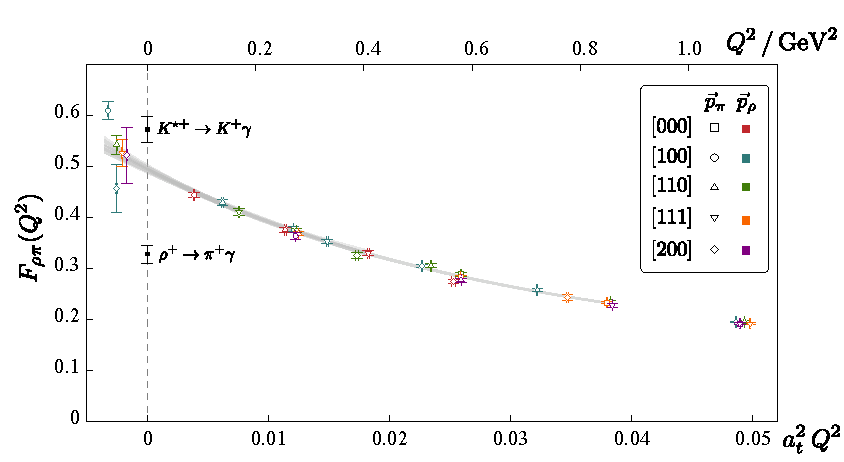
\includegraphics[width=0.8\linewidth]{figures/radTrans/pion_proj0_rho_proj0.pdf}
  \caption{Ground-state $\rho$ to ground-state $\pi$ transition form-factor. Curves in gray show fits used to interpolate between spacelike and timelike regions to determine the photocoupling, $F_{\rho\pi}(0)$. Experimental decay widths converted to photocouplings shown for orientation.  \label{fig::rho_pi_transition}}
    \end{centering}
\end{figure}
\clearpage
}

The $Q^2$ dependence of this meson transition form-factor plays a role in models of deuteron electromagnetic structure, where a virtual photon probe may couple to the bound nucleons or to the meson currents proposed to supply the binding \cite{Arnold:1979cg}.




%%%%%%%%%%%%%%%%%%%%%%%%%%%%%%%%%%%%%%%%%%%%%%%%%%%%%%%%%%%%%%%%%%%%%%%%%%%%%%%%%%%%%%%%%%%%%%%%%%%
\subsubsection{$\rho'\rightarrow\pi\gamma$ transition}
The first-excited $\rho$ state may also undergo a transition to the ground-state pion, with the form of the decomposition of the matrix element being the same as in the previous section. In \secref{sec::Spec:results} we presented the spectrum of excited vector mesons, finding that the first-excited state, $m_{\rho'} = 1882(11) \,\mathrm{MeV}$, is close to being degenerate with the second-excited state $m_{\rho''} = 1992(6) \,\mathrm{MeV}$. Our use of optimized operators corresponding to orthogonal combinations of basis operators allows us to reliably study the two excitations independently. 

We extract the form-factor using optimized operators in correlation functions with time-separation, $\Delta t = 20 \,a_t$, with the results presented in Figure~\ref{fig::rho1_pi_transition}. To determine the photocoupling, $F_{\rho' \pi}(0) = 0.050(4)$, we perform fits to the data over various $Q^2$ ranges using several fit-forms, and the quoted uncertainty includes this variation.

The photocoupling for this transition is observed to be an order of magnitude smaller than that of $\rho \to \pi \gamma$ extracted in Section~\ref{rhopigamma}. Within simple models treating mesons as $q\bar{q}$ bound-states with non-relativistic wavefunctions, such a suppression is expected -- the net effect of the current is to slightly shift in momentum-space the wavefunction of the pion, and since the $\rho'$ is likely described as a radial excitation, the resulting wavefunction overlap is much reduced relative to that for the ground-state $\rho$. This is described as a `hindered' magnetic dipole transition. A relevant experimental example of a hindered transition lies in the charmonium sector -- the relative rates of $\psi(2S) \to \eta_c \gamma$ and $J/\psi \to \eta_c \gamma$, $\frac{\Gamma(\psi(2S) \to \eta_c \gamma)/|\vec{q}_{\psi(2S)}|}{\Gamma(J/\psi \to \eta_c \gamma)/|\vec{q}_{J/\psi}|} \sim 0.1$ show the expected hierarchy of hindered versus non-hindered~\cite{PDG-2012}.


\afterpage{
\begin{figure}[htbp]
\begin{centering}
  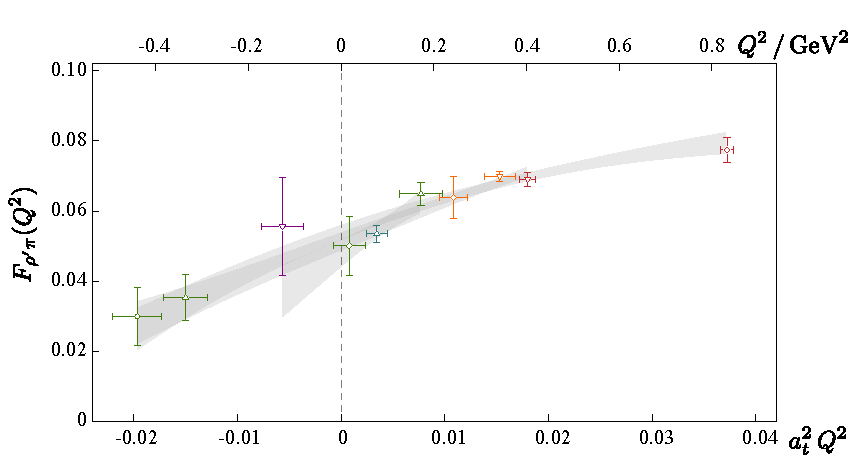
\includegraphics[width=0.8\linewidth]{figures/radTrans/rho_proj1_pion_proj0.pdf}
  \caption{First-excited $\rho$ transition to ground-state $\pi$ form-factor, $F_{\rho'\pi}(Q^2)$. Points have the same color and shape labeling presented in Figure~\ref{fig::rho_pi_transition}. Gray curves show fits used to interpolate to the photocoupling. \label{fig::rho1_pi_transition}}
  \end{centering}
\end{figure}
\clearpage
}




%%%%%%%%%%%%%%%%%%%%%%%%%%%%%%%%%%%%%%%%%%%%%%%%%%%%%%%%%%%%
\subsubsection{$\rho''\rightarrow \pi \gamma$ transition}

An extraction analogous to that presented in the previous subsection can be performed for the second-excited $\rho$ state, leading to the form-factor shown in Figure~\ref{fig::rho2_pi_transition}. Interpolating to $Q^2=0$ using a range of forms yields $F_{\rho'' \pi}(Q^2) = -0.016(3)$, which is smaller still than the $\rho' \to \pi \gamma$ photocoupling. The sign is somewhat arbitrary and would only have definite meaning were we to compare to other transitions involving the $\rho''$.

Within a simple $q\bar{q}$ bound-state model we might expect the $\rho''$ state to be dominated by a $^3\!D_1$ configuration (and indeed the operator overlaps presented in \cite{Dudek:2011bn} seem to suggest this), which would have a `hindered' structure in a transition to the ground-state $S$-wave pseudoscalar owing to the need for the current to provide a $D$-wave angular dependence, which appears only as a relativistic correction to the leading behavior. 

\afterpage{
\begin{figure}[htbp]
\begin{centering}
  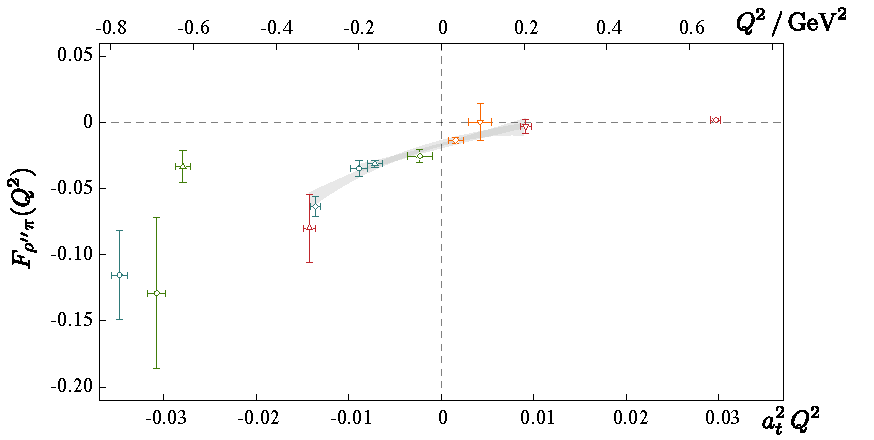
\includegraphics[width=0.8\linewidth]{figures/radTrans/rho_proj2_pion_proj0.pdf}
    \caption{ Second-excited $\rho$ transition to ground-state $\pi$ form-factor, $F_{\rho'' \pi}(Q^2)$. Points have the same color and shape labeling presented in Figure~\ref{fig::rho_pi_transition}. Gray curves show fits used to interpolate to the photocoupling. 
     \label{fig::rho2_pi_transition}}
       \end{centering}
\end{figure}
\clearpage
}




%%%%%%%%%%%%%%%%%%%%%%%%%%%%%%%%%%%%%%%%%%%%%%%%%%%%%%%%%%%%
\subsubsection{$\pi' \rightarrow \rho \gamma$ transition}

The first-excited pion may undergo a transition to the ground-state $\rho$. The results, extracted from $\Delta t = 20 \, a_t$ correlation functions, are presented in Figure~\ref{fig::pi1_rho0_transition}, along with a number of parameterizations used to interpolate a photocoupling of $F_{\pi' \rho}(0) = 0.18(2)$. Again we observe a significant suppression relative to the $\rho \to \pi \gamma$ case in line with this being a hindered transition.

\afterpage{
\begin{figure}[htbp]
\begin{centering}
  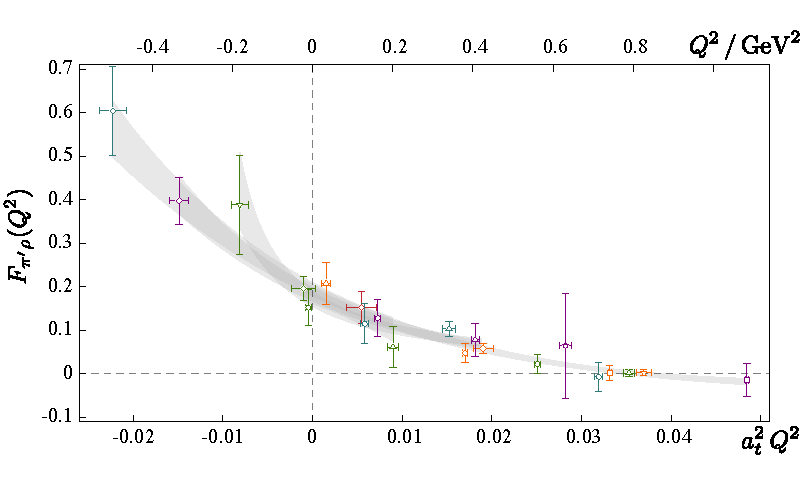
\includegraphics[width=0.8\linewidth]{figures/radTrans/rho_proj0_pion_proj1.pdf}
    \caption{First-excited $\pi$ transition to ground-state $\rho$, $F_{\pi' \rho}(Q^2)$. Gray curves show fits used to interpolate to the photocoupling. \label{fig::pi1_rho0_transition}}
  \end{centering}
\end{figure}
\clearpage
}







%%%%%%%%%%%%%%%%%%%%%%%%%%%%%%%%%%%%%%%%%%%%%%%%%%%%%%%%%%%%
\subsubsection{$\rho' \rightarrow \pi' \gamma$ transition}

This transition, which occurs between excited states, is not expected to be hindered in the case that the $\rho'$ and $\pi'$ are identified predominantly as the first radial excitations of the $\rho$ and $\pi$ respectively. As such we might expect a somewhat larger photocoupling than in previous subsections. We extracted the form-factor from optimized operator correlation functions with $\Delta t = 20 \,a_t$ obtaining the results presented in Figure~\ref{fig::rho1_pi1_transition}. Fits to the $Q^2$ dependence with a range of forms lead to an estimate of the photocoupling, $F_{\rho' \pi'}(Q^2) = 0.7(2)$, which, although not determined with high precision, is of comparable size to the $\rho \to \pi \gamma$ coupling. 

\afterpage{
\begin{figure}[htbp]
\begin{centering}
  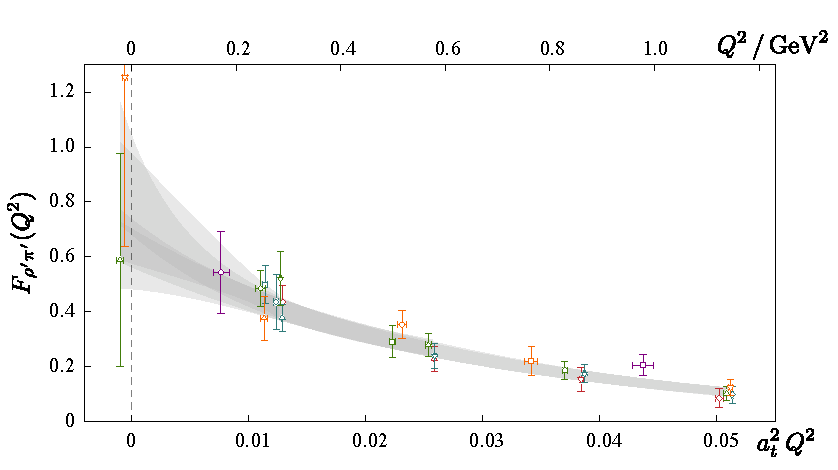
\includegraphics[width=0.8 \linewidth]{figures/radTrans/rho_proj1_pion_proj1.pdf}
      \caption{First-excited $\pi$ transition to first-excited $\rho$, $F_{\pi' \rho'}(Q^2)$. Gray curves show fits used to interpolate to the photocoupling. \label{fig::rho1_pi1_transition}}
        \end{centering}
\end{figure}
\clearpage
}





























\chapter{Concluding Remarks} \label{chap::conclusion}
We started our discussion with an overview of the Standard Model, introducing Quantum Chromodynamics as the relativistic gauge field theory describing the interaction of color charged spin=$\frac{1}{2}$ fermions, quarks, with the spin-$1$ gauge bosons mediating the strong force, gluons. We commented on the non-perturbative nature of QCD which distinguishes it from the other gauge field theories featuring in the standard model -- we don't currently know how to construct analytic solutions to the theory at low energy.  In this manner QCD is perhaps the least understood portion of the Standard Model. 

Historically, a good portion of our intuition comes from models of hadronic physics. These models were built to capture the essential effective degrees of freedom and symmetries present in the experimentally observed spectrum of hadrons. We specifically restricted ourselves to the constituent quark model in which mesons appear as quark-antiquark pairs bound in a central potential of gluonic origin. By constructing $q\bar{q}$ angular momentum eigenstates we were able to illustrate a known result, namely that the predicted spectrum of quark model states, in terms of the $J^{PC}$ quantum numbers is not exhaustive. We identified a set of quantum numbers, $J^{PC} = 0^{--}, (0,2,\ldots)^{+-}, (1,3,\ldots)^{-+}$ known as exotic which may provide hints about the role of glue in Quantum Chromodynamics. 

In order to motivate some of the discussion we also commented on the upcoming GlueX experiments sited at Jefferson Lab which aims to remedy the current lack of photoproduction data in the light quark sector. One of the physics goals of this experiment is to conduct a search for the $J^{PC} =1^{-+}$ exotic states. Currently there is some tentative evidence for three candidate isovector exotic states, $\pi_1(1400), \pi_1(1600), \pi_1(2015)$, though none are without controversy. 

QCD is non-perturbative in this regime; the lattice presents a unique opportunity to provide theoretical input into the expected rate of photo production of exotic mesons. As a first step then we must develop techniques, necessary to extract radiative transition matrix elements directly from the lattice. In the text we show that these matrix elements are embedded in three-point correlation functions, which, in a general sense contain information about many transitions simultaneously. 

Our goal was then to develop analysis methods which allow us to extract a single radiative transition matrix element from a tower of transitions occurring simultaneously. We demonstrated a technique, the construction of optimized interpolating fields, which allow us to project a single contribution out of three point functions, enabling us to study both ground and excited state matrix elements directly on the lattice.  

We then proceeded to use the technique to extract formfactors and transition matrix elements for the lightest few isovector pseudoscalar and vector states in a version of QCD where there are three flavors of quarks all tuned to approximately the physical strange quark mass. Having shown the efficacy of these techniques a natural question is their range of applicability -- where else can we use these methods to study non-perturbative physics?   

One area of immediate interest is in the study of the exotic mesons which motivated a good portion of this work. Here it is a straightforward application of the methods outlined in this manuscript and one could hope to provide some theoretical input about the size of exotic photo couplings in the near term future. 

The techniques outlined can also be generalized quite readily to the baryon sector. In this case one might be interested in reactions such as $N^* \rightarrow N^* \gamma$ as a method to study the internal quark structure of excited baryons non-perturbatively. Also of interest are transitions involving nucleons, for example, $N^*\rightarrow N \gamma$ where the dependence of the transition form factor on the photon virtuality can be measured quite directly in electroproduction experiments. 

From a more theoretical perspective, these techniques are also quite interesting when applied to unstable particles. Throughout this analysis we have been working under the assumption that our states are stable. In general this is not always true, for example the $\rho$ meson occurs as a dynamically generated resonance in $\pi\pi$ scattering. On the lattice this introduces additional complications associated with form factor extraction. To date, however, there is no calculation exploring the coupling of a resonance to external currents. A rigorous calculation at physical kinematics, where the $\rho$ is a resonance, seeking the coupling $\rho\rightarrow\pi\gamma$ would in fact need to determine the P-wave partial-wave amplitude for $\pi\pi \rightarrow \pi \gamma$ as a function of the invariant mass, $m_{\pi\pi}$. By analytically continuing the amplitude to complex values of $m^2_{\pi\pi}$ and extrapolating to the $\rho$-resonance pole, the coupling could be extracted as the residue of the amplitude. Very recently \cite{Briceno:2014uqa} the formalism relating matrix elements extracted in a finite volume to the physical amplitude has been developed. Calculations aiming to extract the value of the  $\pi\pi \rightarrow \pi \gamma$ at the $\rho$-meson pole using the techniques outlined in this analysis are currently underway.

In short, the techniques laid out in this dissertation, allowing for the extraction of single matrix elements for each state in a tower of discrete eigenstates, are required for any attempt to determine excited state or resonance couplings to external currents aiming to probe these states. The technical formalism has now been implemented and explored; more complicated three-point function calculations can now be attempted. 






  %This begins the list of reference or bibliography. The default form is consistent
  %with the references in the Physical Review. The articles must be listed in the order
  %in which they appear in the text. The style of the bibliography can be changed and
  %automatic ordering of the entries can be accomplished using BibTeX. Use of BibTeX is
  %explained in most of the standard LaTeX books.

%%%%%%%%%%%%% OUT WITH THE OLD
%\bibliographystyle{plain}
%\begin{thebibliography}{99}
%\addtocontents{toc}{\vspace*{12pt}}  %This command adds some extra space in the table of
                                     %contents
%\addcontentsline{toc}{chapter}{BIBLIOGRAPHY}  %This command adds and entry for the
                                              %bibliography in the table of contents
%
\bibitem{Ablikim:2011da}
M.~Ablikim et~al.
\newblock {Higher-order multipole amplitude measurement in
  $\psi(2S)\to\gamma\chi_{c2}$}.
\newblock {\em Phys.Rev.}, D84:092006, 2011.

\bibitem{Ablikim:2011kv}
M.~Ablikim et~al.
\newblock {Study of $\chi_{cJ}$ radiative decays into a vector meson}.
\newblock {\em Phys.Rev.}, D83:112005, 2011.

\bibitem{Ablikim:2012sf}
M.~Ablikim et~al.
\newblock {First observation of the M1 transition $\psi(3686)\to
  \gamma\eta_c(2S)$}.
\newblock {\em Phys.Rev.Lett.}, 109:042003, 2012.

\bibitem{Ablikim:2013hq}
M.~Ablikim et~al.
\newblock {Partial wave analysis of $J/\psi \to \gamma \eta \eta$}.
\newblock {\em Phys.Rev.}, D87(9):092009, 2013.

\bibitem{Adolph:2014mup}
C.~Adolph et~al.
\newblock {Measurement of radiative widths of $a_2(1320)$ and $\pi_2(1670)$}.
\newblock {\em Eur.Phys.J.}, A50:79, 2014.

\bibitem{PhysRevD.83.045010}
C.~Alexandrou, M.~Brinet, J.~Carbonell, M.~Constantinou, P.~A. Harraud,
  P.~Guichon, K.~Jansen, T.~Korzec, and M.~Papinutto.
\newblock Axial nucleon form factors from lattice qcd.
\newblock {\em Phys. Rev. D}, 83:045010, Feb 2011.

\bibitem{Allton:1993wc}
C.R. Allton et~al.
\newblock {Gauge invariant smearing and matrix correlators using Wilson
  fermions at Beta = 6.2}.
\newblock {\em Phys.Rev.}, D47:5128--5137, 1993.

\bibitem{Amendolia:1986ui}
S.R. Amendolia, G.~Batignani, G.A. Beck, E.H. Bellamy, E.~Bertolucci, et~al.
\newblock {A Measurement of the Kaon Charge Radius}.
\newblock {\em Phys.Lett.}, B178:435, 1986.

\bibitem{Amendolia:1986wj}
S.R. Amendolia et~al.
\newblock {A Measurement of the Space - Like Pion Electromagnetic Form-Factor}.
\newblock {\em Nucl.Phys.}, B277:168, 1986.

\bibitem{Arnold:1979cg}
R.G. Arnold, Carl~E. Carlson, and Franz Gross.
\newblock {Elastic electron-Deuteron Scattering at High-Energy}.
\newblock {\em Phys.Rev.}, C21:1426, 1980.

\bibitem{Aznauryan:2012ba}
I.G. Aznauryan, A.~Bashir, V.~Braun, S.J. Brodsky, V.D. Burkert, et~al.
\newblock {Studies of Nucleon Resonance Structure in Exclusive Meson
  Electroproduction}.
\newblock {\em Int.J.Mod.Phys.}, E22:1330015, 2013.

\bibitem{Babich:2010mu}
Ronald Babich, Michael~A. Clark, and Balint Joo.
\newblock {Parallelizing the QUDA Library for Multi-GPU Calculations in Lattice
  Quantum Chromodynamics}.
\newblock {\em {ACM/IEEE Int. Conf. High Performance Computing, Networking,
  Storage and Analysis, New Orleans}}, 2010.

\bibitem{Bali:2014gha}
Gunnar~S. Bali, Sara Collins, Benjamin Gl��le, Meinulf G�ckeler, Johannes
  Najjar, et~al.
\newblock {The moment $\langle x\rangle_{u-d}$ of the nucleon from $N_f=2$
  lattice QCD down to nearly physical quark masses}.
\newblock 2014.

\bibitem{Barnes:1982tx}
Ted Barnes, F.E. Close, F.~de~Viron, and J.~Weyers.
\newblock {Q anti-Q G Hermaphrodite Mesons in the MIT Bag Model}.
\newblock {\em Nucl.Phys.}, B224:241, 1983.

\bibitem{PDG-2012}
J.~Beringer et~al.
\newblock Review of particle physics.
\newblock {\em Phys. Rev. D}, 86:010001, 2012.

\bibitem{Blossier:2009kd}
Benoit Blossier, Michele Della~Morte, Georg von Hippel, Tereza Mendes, and
  Rainer Sommer.
\newblock {On the generalized eigenvalue method for energies and matrix
  elements in lattice field theory}.
\newblock {\em JHEP}, 0904:094, 2009.

\bibitem{Briceno:2014pka}
Ra�l~A. Brice�o.
\newblock {Few-body physics}.
\newblock 2014.

\bibitem{Briceno:2014uqa}
Ra�l~A. Brice�o, Maxwell~T. Hansen, and Andr� Walker-Loud.
\newblock {Multichannel one-to-two transition form factors in a finite volume}.
\newblock 2014.

\bibitem{Bulava:2010yg}
J.~Bulava, R.G. Edwards, E.~Engelson, B.~Joo, H-W. Lin, et~al.
\newblock {Nucleon, $\Delta$ and $\Omega$ excited states in $N_f=2+1$ lattice
  QCD}.
\newblock {\em Phys.Rev.}, D82:014507, 2010.

\bibitem{Bulava:2010vk}
John Bulava, Robert~G. Edwards, Balint Joo, David~G. Richards, Eric Engelson,
  et~al.
\newblock {Nucleon, Delta and Omega excited state spectra at three pion mass
  values}.
\newblock {\em PoS}, LATTICE2010:129, 2010.

\bibitem{Capraro:1987rp}
L.~Capraro, P.~Levy, M.~Querrou, B.~Van~Hecke, M.~Verbeken, et~al.
\newblock {The $\rho$ Radiative Decay Width: A Measurement at 200-{GeV}}.
\newblock {\em Nucl.Phys.}, B288:659, 1987.

\bibitem{PhysRevLett.51.168}
C.~Chandlee, D.~Berg, S.~Cihangir, B.~Collick, T.~Ferbel, S.~Heppelmann,
  J.~Huston, T.~Jensen, A.~Jonckheere, F.~Lobkowicz, Y.~Makdisi, M.~Marshak,
  M.~McLaughlin, C.~Nelson, T.~Ohshima, E.~Peterson, K.~Ruddick, P.~Slattery,
  P.~Thompson, and M.~Zielinski.
\newblock Measurement of the radiative width of the ${K}^{*+}(890)$.
\newblock {\em Phys. Rev. Lett.}, 51:168--171, Jul 1983.

\bibitem{Chanowitz:1982qj}
Michael~S. Chanowitz and Stephen~R. Sharpe.
\newblock {Hybrids: Mixed States of Quarks and Gluons}.
\newblock {\em Nucl.Phys.}, B222:211, 1983.

\bibitem{Chen:2000ej}
Ping Chen.
\newblock {Heavy quarks on anisotropic lattices: The Charmonium spectrum}.
\newblock {\em Phys.Rev.}, D64:034509, 2001.

\bibitem{Clark:2009wm}
M.~A. Clark et~al.
\newblock {Solving Lattice QCD systems of equations using mixed precision
  solvers on GPUs}.
\newblock {\em Comput. Phys. Commun.}, 181:1517--1528, 2010.

\bibitem{Close:2003fz}
F.E. Close and J.J. Dudek.
\newblock {Electroweak production of hybrid mesons in a flux tube simulation of
  lattice QCD}.
\newblock {\em Phys.Rev.Lett.}, 91:142001, 2003.

\bibitem{Close:2003ae}
F.E. Close and J.J. Dudek.
\newblock {Hybrid meson production by electromagnetic and weak interactions in
  a flux tube simulation of lattice QCD}.
\newblock {\em Phys.Rev.}, D69:034010, 2004.

\bibitem{Davoudi:2012ya}
Zohreh Davoudi and Martin~J. Savage.
\newblock {Restoration of Rotational Symmetry in the Continuum Limit of Lattice
  Field Theories}.
\newblock {\em Phys.Rev.}, D86:054505, 2012.

\bibitem{Dinter:2011sg}
Simon Dinter, Constantia Alexandrou, Martha Constantinou, Vincent Drach, Karl
  Jansen, et~al.
\newblock {Precision Study of Excited State Effects in Nucleon Matrix
  Elements}.
\newblock {\em Phys.Lett.}, B704:89--93, 2011.

\bibitem{Djukanovic:2013mka}
D.~Djukanovic, E.~Epelbaum, J.~Gegelia, and U.-G. Meissner.
\newblock {The magnetic moment of the $\rho$-meson}.
\newblock {\em Phys.Lett.}, B730:115--121, 2014.

\bibitem{Dudek:2012vr}
Jozef Dudek, Rolf Ent, Rouven Essig, K.S. Kumar, Curtis Meyer, et~al.
\newblock {Physics Opportunities with the 12 GeV Upgrade at Jefferson Lab}.
\newblock {\em Eur.Phys.J.}, A48:187, 2012.

\bibitem{Dudek:2011bn}
Jozef~J. Dudek.
\newblock {The lightest hybrid meson supermultiplet in QCD}.
\newblock {\em Phys.Rev.}, D84:074023, 2011.

\bibitem{Dudek:2009kk}
Jozef~J. Dudek, Robert Edwards, and Christopher~E. Thomas.
\newblock {Exotic and excited-state radiative transitions in charmonium from
  lattice QCD}.
\newblock {\em Phys.Rev.}, D79:094504, 2009.

\bibitem{Dudek:2012ag}
Jozef~J. Dudek and Robert~G. Edwards.
\newblock {Hybrid Baryons in QCD}.
\newblock {\em Phys.Rev.}, D85:054016, 2012.

\bibitem{Dudek:2013yja}
Jozef~J. Dudek, Robert~G. Edwards, Peng Guo, and Christopher~E. Thomas.
\newblock {Toward the excited isoscalar meson spectrum from lattice QCD}.
\newblock {\em Phys.Rev.}, D88(9):094505, 2013.

\bibitem{Dudek:2011tt}
Jozef~J. Dudek, Robert~G. Edwards, Balint Joo, Michael~J. Peardon, David~G.
  Richards, et~al.
\newblock {Isoscalar meson spectroscopy from lattice QCD}.
\newblock {\em Phys.Rev.}, D83:111502, 2011.

\bibitem{Dudek:2007wv}
Jozef~J. Dudek, Robert~G. Edwards, Nilmani Mathur, and David~G. Richards.
\newblock {Charmonium excited state spectrum in lattice QCD}.
\newblock {\em Phys.Rev.}, D77:034501, 2008.

\bibitem{Dudek:2009qf}
Jozef~J. Dudek, Robert~G. Edwards, Michael~J. Peardon, David~G. Richards, and
  Christopher~E. Thomas.
\newblock {Highly excited and exotic meson spectrum from dynamical lattice
  QCD}.
\newblock {\em Phys.Rev.Lett.}, 103:262001, 2009.

\bibitem{Dudek:2010wm}
Jozef~J. Dudek, Robert~G. Edwards, Michael~J. Peardon, David~G. Richards, and
  Christopher~E. Thomas.
\newblock {Toward the excited meson spectrum of dynamical QCD}.
\newblock {\em Phys.Rev.}, D82:034508, 2010.

\bibitem{Dudek:2010ew}
Jozef~J. Dudek, Robert~G. Edwards, Michael~J. Peardon, David~G. Richards, and
  Christopher~E. Thomas.
\newblock {The phase-shift of isospin-2 pi-pi scattering from lattice QCD}.
\newblock {\em Phys.Rev.}, D83:071504, 2011.

\bibitem{Dudek:2006ej}
Jozef~J. Dudek, Robert~G. Edwards, and David~G. Richards.
\newblock {Radiative transitions in charmonium from lattice QCD}.
\newblock {\em Phys.Rev.}, D73:074507, 2006.

\bibitem{PhysRevD.79.094504}
Jozef~J. Dudek, Robert~G. Edwards, and Christopher~E. Thomas.
\newblock Exotic and excited-state radiative transitions in charmonium from
  lattice qcd.
\newblock {\em Phys. Rev. D}, 79:094504, May 2009.

\bibitem{Dudek:2012gj}
Jozef~J. Dudek, Robert~G. Edwards, and Christopher~E. Thomas.
\newblock {S and D-wave phase shifts in isospin-2 pi pi scattering from lattice
  QCD}.
\newblock {\em Phys.Rev.}, D86:034031, 2012.

\bibitem{Dudek:2012xn}
Jozef~J. Dudek, Robert~G. Edwards, and Christopher~E. Thomas.
\newblock {Energy dependence of the $\rho$ resonance in $\pi\pi$ elastic
  scattering from lattice QCD}.
\newblock {\em Phys.Rev.}, D87(3):034505, 2013.

\bibitem{Dudek:2014qha}
Jozef~J. Dudek, Robert~G. Edwards, Christopher~E. Thomas, and David~J. Wilson.
\newblock {Resonances in coupled $\pi K -\eta K$ scattering from quantum
  chromodynamics}.
\newblock {\em Phys.Rev.Lett.}, 113(18):182001, 2014.

\bibitem{Durand:1962zza}
Loyal Durand, Paul~C. DeCelles, and Robert~B. Marr.
\newblock {Lorentz Invariance and the Kinematic Structure of Vertex Functions}.
\newblock {\em Phys.Rev.}, 126:1882--1898, 1962.

\bibitem{PhysRevLett.96.052001}
R.~G. Edwards, G.~T. Fleming, Ph. H\"agler, J.~W. Negele, K.~Orginos, A.~V.
  Pochinsky, D.~B. Renner, D.~G. Richards, and W.~Schroers.
\newblock Nucleon axial charge in full lattice qcd.
\newblock {\em Phys. Rev. Lett.}, 96:052001, Feb 2006.

\bibitem{Edwards:2011jj}
Robert~G. Edwards, Jozef~J. Dudek, David~G. Richards, and Stephen~J. Wallace.
\newblock {Excited state baryon spectroscopy from lattice QCD}.
\newblock {\em Phys.Rev.}, D84:074508, 2011.

\bibitem{Edwards:2004sx}
Robert~G. Edwards and Balint Joo.
\newblock {The Chroma software system for lattice QCD}.
\newblock {\em Nucl.Phys.Proc.Suppl.}, 140:832, 2005.

\bibitem{Edwards:2008ja}
Robert~G. Edwards, Balint Joo, and Huey-Wen Lin.
\newblock {Tuning for Three-flavors of Anisotropic Clover Fermions with
  Stout-link Smearing}.
\newblock {\em Phys.Rev.}, D78:054501, 2008.

\bibitem{Edwards:2012fx}
Robert~G. Edwards, Nilmani Mathur, David~G. Richards, and Stephen~J. Wallace.
\newblock {Flavor structure of the excited baryon spectra from lattice QCD}.
\newblock {\em Phys.Rev.}, D87(5):054506, 2013.

\bibitem{Feng:2014gba}
Xu~Feng, Sinya Aoki, Shoji Hashimoto, and Takashi Kaneko.
\newblock {Time-like pion form factor in lattice QCD}.
\newblock 2014.

\bibitem{Feng:2010es}
Xu~Feng, Karl Jansen, and Dru~B. Renner.
\newblock {Resonance Parameters of the rho-Meson from Lattice QCD}.
\newblock {\em Phys.Rev.}, D83:094505, 2011.

\bibitem{Flynn:2005in}
J.M. Flynn, A.~Juttner, and C.T. Sachrajda.
\newblock {A Numerical study of partially twisted boundary conditions}.
\newblock {\em Phys.Lett.}, B632:313--318, 2006.

\bibitem{Green:2014xba}
J.R. Green, J.W. Negele, A.V. Pochinsky, S.N. Syritsyn, M.~Engelhardt, et~al.
\newblock {Nucleon electromagnetic form factors from lattice QCD using a nearly
  physical pion mass}.
\newblock {\em Phys.Rev.}, D90(7):074507, 2014.

\bibitem{Gusken:1989ad}
S.~Gusken, U.~Low, K.H. Mutter, R.~Sommer, A.~Patel, et~al.
\newblock {Nonsinglet Axial Vector Couplings of the Baryon Octet in Lattice
  {QCD}}.
\newblock {\em Phys.Lett.}, B227:266, 1989.

\bibitem{Hedditch:2007ex}
J.N. Hedditch, W.~Kamleh, B.G. Lasscock, D.B. Leinweber, A.G. Williams, et~al.
\newblock {Pseudoscalar and vector meson form-factors from lattice QCD}.
\newblock {\em Phys.Rev.}, D75:094504, 2007.

\bibitem{Horn:1977rq}
D.~Horn and J.~Mandula.
\newblock {A Model of Mesons with Constituent Gluons}.
\newblock {\em Phys.Rev.}, D17:898, 1978.

\bibitem{Horsley:2013ayv}
R.~Horsley, Y.~Nakamura, A.~Nobile, P.E.L. Rakow, G.~Schierholz, et~al.
\newblock {Nucleon axial charge and pion decay constant from two-flavor lattice
  QCD}.
\newblock {\em Phys.Lett.}, B732:41--48, 2014.

\bibitem{PhysRevD.33.3199}
J.~Huston, D.~Berg, C.~Chandlee, S.~Cihangir, T.~Ferbel, T.~Jensen,
  F.~Lobkowicz, M.~McLaughlin, T.~Ohshima, P.~Slattery, P.~Thompson,
  M.~Zielinski, B.~Collick, S.~Heppelmann, Y.~Makdisi, M.~Marshak, E.~Peterson,
  K.~Ruddick, A.~Jonckheere, and C.~Nelson.
\newblock Measurement of the resonance parameters and radiative width of the
  $\rho^+$.
\newblock {\em Phys. Rev. D}, 33:3199--3202, Jun 1986.

\bibitem{Isgur:1999kx}
Nathan Isgur.
\newblock {Flux tube zero point motion, hadronic charge radii, and hybrid meson
  production cross-sections}.
\newblock {\em Phys.Rev.}, D60:114016, 1999.

\bibitem{Isgur:1985vy}
Nathan Isgur, Richard Kokoski, and Jack~E. Paton.
\newblock {Gluonic Excitations of Mesons: Why They Are Missing and Where to
  Find Them}.
\newblock {\em Phys.Rev.Lett.}, 54:869, 1985.

\bibitem{Ito:1993au}
Hiroshi Ito and Franz Gross.
\newblock {Isoscalar meson exchange currents and the deuteron form-factors}.
\newblock {\em Phys.Rev.Lett.}, 71:2555--2558, 1993.

\bibitem{Kim:2005gf}
C.h. Kim, C.T. Sachrajda, and Stephen~R. Sharpe.
\newblock {Finite-volume effects for two-hadron states in moving frames}.
\newblock {\em Nucl.Phys.}, B727:218--243, 2005.

\bibitem{Lee:2008qf}
Frank~X. Lee, Scott Moerschbacher, and Walter Wilcox.
\newblock {Magnetic moments of vector, axial, and tensor mesons in lattice
  QCD}.
\newblock {\em Phys.Rev.}, D78:094502, 2008.

\bibitem{Lin:2012ev}
Huey-Wen Lin.
\newblock {Lattice Hadron Structure: Applications within and beyond QCD}.
\newblock {\em PoS}, LATTICE2012:013, 2012.

\bibitem{Lin:2008pr}
Huey-Wen Lin et~al.
\newblock {First results from 2+1 dynamical quark flavors on an anisotropic
  lattice: Light-hadron spectroscopy and setting the strange-quark mass}.
\newblock {\em Phys.Rev.}, D79:034502, 2009.

\bibitem{Liu:2012ze}
Liuming Liu et~al.
\newblock {Excited and exotic charmonium spectroscopy from lattice QCD}.
\newblock {\em JHEP}, 1207:126, 2012.

\bibitem{Luscher:1986pf}
M.~Luscher.
\newblock {Volume Dependence of the Energy Spectrum in Massive Quantum Field
  Theories. 2. Scattering States}.
\newblock {\em Commun.Math.Phys.}, 105:153--188, 1986.

\bibitem{Luscher:1990ux}
Martin L\"uscher.
\newblock {Two particle states on a torus and their relation to the scattering
  matrix}.
\newblock {\em Nucl.Phys.}, B354:531--578, 1991.

\bibitem{Luscher:1990ck}
Martin Luscher and Ulli Wolff.
\newblock {How to Calculate the Elastic Scattering Matrix in Two-dimensional
  Quantum Field Theories by Numerical Simulation}.
\newblock {\em Nucl.Phys.}, B339:222--252, 1990.

\bibitem{Mastropas:2014fsa}
Ekaterina~V. Mastropas and David~G. Richards.
\newblock {Decay constants of the pion and its excitations on the lattice}.
\newblock {\em Phys.Rev.}, D90:014511, 2014.

\bibitem{Meyer:2011um}
Harvey~B. Meyer.
\newblock {Lattice QCD and the Timelike Pion Form Factor}.
\newblock {\em Phys.Rev.Lett.}, 107:072002, 2011.

\bibitem{Michael:1985ne}
Christopher Michael.
\newblock {Adjoint Sources in Lattice Gauge Theory}.
\newblock {\em Nucl.Phys.}, B259:58, 1985.

\bibitem{Mohler:2012nh}
Daniel Mohler.
\newblock {Review of lattice studies of resonances}.
\newblock {\em PoS}, LATTICE2012:003, 2012.

\bibitem{Moore:2006ng}
David~C. Moore and George~T. Fleming.
\newblock {Multiparticle States and the Hadron Spectrum on the Lattice}.
\newblock {\em Phys.Rev.}, D74:054504, 2006.

\bibitem{Moore:2005dw}
David~C. Moore and George~Tamminga Fleming.
\newblock {Angular momentum on the lattice: The Case of non-zero linear
  momentum}.
\newblock {\em Phys.Rev.}, D73:014504, 2006.

\bibitem{Morningstar:1999dh}
Colin Morningstar and Mike~J. Peardon.
\newblock {The Glueball spectrum from novel improved actions}.
\newblock {\em Nucl.Phys.Proc.Suppl.}, 83:887--889, 2000.

\bibitem{Morningstar:1999rf}
Colin~J. Morningstar and Mike~J. Peardon.
\newblock {The Glueball spectrum from an anisotropic lattice study}.
\newblock {\em Phys.Rev.}, D60:034509, 1999.

\bibitem{Owen:2015gva}
Benjamin Owen, Waseem Kamleh, Derek Leinweber, Benjamin Menadue, and Selim
  Mahbub.
\newblock {Light Meson Form Factors at near Physical Masses}.
\newblock 2015.

\bibitem{Padmanath:2013zfa}
M.~Padmanath, Robert~G. Edwards, Nilmani Mathur, and Michael Peardon.
\newblock {Spectroscopy of triply-charmed baryons from lattice QCD}.
\newblock {\em Phys.Rev.}, D90:074504, 2014.

\bibitem{Peardon:2009gh}
Michael Peardon et~al.
\newblock {A Novel quark-field creation operator construction for hadronic
  physics in lattice QCD}.
\newblock {\em Phys.Rev.}, D80:054506, 2009.

\bibitem{0201503972}
Michael~E. Peskin and Dan~V. Schroeder.
\newblock {\em An Introduction To Quantum Field Theory (Frontiers in Physics)}.
\newblock Westview Press, 1995.

\bibitem{Prelovsek:2014zga}
Sasa Prelovsek.
\newblock {Hadron Spectroscopy}.
\newblock {\em PoS}, LATTICE2014:015, 2014.

\bibitem{Rummukainen:1995vs}
K.~Rummukainen and Steven~A. Gottlieb.
\newblock {Resonance scattering phase shifts on a nonrest frame lattice}.
\newblock {\em Nucl.Phys.}, B450:397--436, 1995.

\bibitem{Shultz:2015pfa}
Christian~J. Shultz, Jozef~J. Dudek, and Robert~G. Edwards.
\newblock {Excited meson radiative transitions from lattice QCD using
  variationally optimized operators}.
\newblock 2015.

\bibitem{Symanzik:1983dc}
K.~Symanzik.
\newblock {Continuum Limit and Improved Action in Lattice Theories. 1.
  Principles and phi**4 Theory}.
\newblock {\em Nucl.Phys.}, B226:187, 1983.

\bibitem{Thomas:2011rh}
Christopher~E. Thomas, Robert~G. Edwards, and Jozef~J. Dudek.
\newblock {Helicity operators for mesons in flight on the lattice}.
\newblock {\em Phys.Rev.}, D85:014507, 2012.

\bibitem{PhysRevLett.100.171602}
T.~Yamazaki, Y.~Aoki, T.~Blum, H.~W. Lin, M.~F. Lin, S.~Ohta, S.~Sasaki, R.~J.
  Tweedie, and J.~M. Zanotti.
\newblock Nucleon axial charge in ($2+1$)-flavor dynamical-lattice qcd with
  domain-wall fermions.
\newblock {\em Phys. Rev. Lett.}, 100:171602, Apr 2008.


%\end{thebibliography}

%%%%%%%% this seems to cause the bib to mess itself up??
\addtocontents{toc}{\vspace*{12pt}}  %This command adds some extra space in the table of
                                     %contents
\addcontentsline{toc}{chapter}{BIBLIOGRAPHY}  %This command adds and entry for the
                                              %bibliography in the table of contents

\bibliographystyle{plain}
%\bibliographystyle{unsrt}
%\bibliographystyle{unsrtnat}
%\bibliographystyle{apsrev4-1}
%\bibliographystyle{alpha}
\bibliography{bib}




%This command begins the Appendix section. The style of the chapter numbering is changed to
%letters

\appendix

\chapter{Methods}


%%%%%%%%%%%%%%%%%%%%%%%%%%%%%%%%%%%%%%%%%%%%%%%%%%%%%%%%%
%%%%%%%%%%%%%%%%%%%%%%%%%%%%%%%%%%%%%%%%%%%%%%%%%%%%%%%%%
%%%%%%%%%%%%%%%%%%%%%%%%%%%%%%%%%%%%%%%%%%%%%%%%%%%%%%%%% 
 
\section{Grassman Numbers}\label{app::grassman}
The generators of an n-dimensional Grassman Algebra obey the anti-commutation relation 
\begin{equation*}
\{G_i,G_j\} \equiv G_iG_j + G_jG_i = 0 \qquad G_i^2 = 0
\end{equation*}
where $i,j=1,2,...,n$. Because of the anti-commutation relation the expansion of any function defined on a finite Grassman Algebra contains only a finite number of terms (any term quadratic or higher in a single generator is zero). We define integration of Grassman quantities as 
\begin{equation*}
\int dG_i = 0 \qquad \int dG_iG_i = 1 \qquad \{G_i,dG_j\} = 0 \qquad \{dG_i,dG_j\} = 0
\end{equation*}
For example let $g$ and $\bar{g}$ be independent Grassman quantities, then 
\begin{equation*}
\int dg = \int d\bar{g} = 0 \qquad \int dgg = \int d\bar{g}\bar{g} = 1.
\end{equation*}
Since $gg = \bar{g}\bar{g} = 0$ we see 
\begin{equation*}
e^{g\bar{g}} = 1 + g\bar{g}
\end{equation*}
and thus 
\begin{align*}
\int dgd\bar{g}e^{g\bar{g}} &= \int dgd\bar{g} + \int dgd\bar{g} g\bar{g} \notag \\
&= 0 - \int dgg d\bar{g}\bar{g} \notag \\
&= -1
\end{align*}
Where we have used the relation $\{G_i,dG_j\} = 0$ to pick up the minus sign in the second line. Now we consider a two dimensional case, 
\begin{equation*}
g = \left(\begin{array}{c} g_1 \\ g_2 \end{array} \right), \qquad \bar{g} = \left(\begin{array}{c} \bar{g}_1 \\ \bar{g}_2 \end{array}\right), \qquad g^T\bar{g} = g_1\bar{g}_1 + g_2\bar{g}_2
\end{equation*}
Then one can verify that 
\begin{equation*}
e^{-g^T\bar{g}} = 1 - (g_1\bar{g}_1 + g_2\bar{g}_2) + g_1\bar{g}_1g_2\bar{g}_2.
\end{equation*}
Defining the integration rule $dgd\bar{g} = dg_1d\bar{g}_1dg_2d\bar{g}_2$ we see then that 
\begin{equation*}
\int dgd\bar{g}e^{-g^T\bar{g}} = 1.
\end{equation*}
Performing a change of variables $g = M\xi$ and $\bar{g} = M^{\prime}\bar{\xi}$ then 
\begin{equation*}
\left(\begin{array}{c} g_1 \\ g_2 \end{array}\right) = 
\left(\begin{array}{cc} M_{11} & M_{12} \\ M_{21} & M_{22} \end{array} \right) 
\left(\begin{array}{c} \xi_1 \\ \xi_2 \end{array} \right) =
\left(\begin{array}{c} M_{11}\xi_1 + M_{12}\xi_2 \\ M_{21}\xi_1 + M_{22}\xi_2 \end{array} \right).
\end{equation*} 
So then we can compute 
\begin{align*}
g_1g_2 &= (M_{11}\xi_1 + M_{12}\xi_2)(M_{21}\xi_1 + M_{22}\xi_2) \notag \\
&= M_{11}M_{22}\xi_1\xi_2 + M_{12}M_{21}\xi_2\xi_1 \notag \\
&= M_{11}M_{22}\xi_1\xi_2 - M_{12}M_{21}\xi_1\xi_2 \notag \\
&= \mathrm{det}(M)\xi_1\xi_2. 
\end{align*}
In order to preserve integration under change of variables then we require
\begin{equation*}
\int dg_1dg_2g_1g_2 = \int d\xi_1 d\xi_2 \xi_1 \bar{\xi}_2 \quad \longrightarrow \quad dg_1dg_2 = \mathrm{det}(M)^{-1}d\xi_1d\xi_2.
\end{equation*}
It follows by substitution that 
\begin{equation*}
1 = \int dgd\bar{g}e^{-g^T\bar{g}} = (\mathrm{det}(M^T)\mathrm{det}(M^{\prime}))^{-1} \int d\xi d\bar{\xi}e^{\xi^TM^TM^{\prime}\bar{\xi}}.
\end{equation*}
Defining $\tilde{M}\equiv M^TM^{\prime}$ and using the relations $\mathrm{det}(M^T) = \mathrm{det}(M)$ and $\mathrm{det}(AB) = \mathrm{det}(A)\mathrm{det}(B)$ we find 
\begin{equation*}
\int d\xi d\bar{\xi}e^{\xi^T\tilde{M}\bar{\xi}}  = \mathrm{det}(\tilde{M}).
\end{equation*}
This formula generalizes to the case where $\xi$ and $\bar{\xi}$ are vectors of arbitrary length.

%%%%%%%%%%%%%%%%%%%%%%%%%%%%%%%%%%%%%%%%%%%%%%%%%%%%%%%%%
%%%%%%%%%%%%%%%%%%%%%%%%%%%%%%%%%%%%%%%%%%%%%%%%%%%%%%%%%
%%%%%%%%%%%%%%%%%%%%%%%%%%%%%%%%%%%%%%%%%%%%%%%%%%%%%%%%% 




%%%%%%%%%%%%%%%%%%%%%%%%%%%%%%%%%%%%%%%%%%%%%%%%%%%%%%%%%
%%%%%%%%%%%%%%%%%%%%%%%%%%%%%%%%%%%%%%%%%%%%%%%%%%%%%%%%%
%%%%%%%%%%%%%%%%%%%%%%%%%%%%%%%%%%%%%%%%%%%%%%%%%%%%%%%%% 

\section{Single Elimination Jackknife Statistics \label{App:jack}}
Given some statistical sample $y_i \in \left\{{Y}\right\}$ the mean and variance are defined
\begin{align*}
\bar{y} &= \frac{1}{N}\sum_i^Ny_i \\
var(y) &= \frac{1}{N}\sum_i^N \left(y_i - \bar{y}\right)^2
\end{align*}
In order to propagate the error using the jackknife method one takes the sample $y_i$ in what is called ensemble data format (a list of samples) and converts it to the jackknife format by
\begin{align*}
y^{jack.}_i &= \frac{1}{N-1}\sum_{j\ne i}^N y_j \\
&= \bar{y} - \frac{1}{N-1}\left(y_i - \bar{y}\right).
\end{align*}
By inspection one realizes that the jackknife rescaled data will have the same mean as the ensemble format data. The effect is to scale down the fluctuations by a factor of $\frac{1}{N-1}$.  One then calculates some function of the samples in the jackknife format and then inverts the rescaling to obtain the distribution in the ensemble format.
\begin{align*}
f^{jack.}_i &= g\left(y^{jack.}_i,z^{jack.}_i,\cdots\right)\\
f_i &= \bar{f} - \frac{1}{N-1}\left(f_i^{jack.}-\bar{f}\right)
\end{align*}
The variance of the ensemble of samples $f_i$ is then given by the standard formula.








\chapter{Spectroscopy}


%%%%%%%%%%%%%%%%%%%%%%%%%%%%%%%%%%%%%%%%%%%%%%%%%%%%%%%%%
%%%%%%%%%%%%%%%%%%%%%%%%%%%%%%%%%%%%%%%%%%%%%%%%%%%%%%%%%
%%%%%%%%%%%%%%%%%%%%%%%%%%%%%%%%%%%%%%%%%%%%%%%%%%%%%%%%%


%%%%%%%%%%%%%%%%%%%%%%%%%%%%%%%%%%%%%%%%%%%%%%%%%%%%%%%%%
%%%%%%%%%%%%%%%%%%%%%%%%%%%%%%%%%%%%%%%%%%%%%%%%%%%%%%%%%
%%%%%%%%%%%%%%%%%%%%%%%%%%%%%%%%%%%%%%%%%%%%%%%%%%%%%%%%%

\section{Generalized Eigenvalue Problem}\label{app::GEVP}


%%%%%%%%%%%%%%%%%%%%%%%%%%%%%%%%%%%%%%%%%%%%%%%%%%%%%%%%%
%%%%%%%%%%%%%%%%%%%%%%%%%%%%%%%%%%%%%%%%%%%%%%%%%%%%%%%%%
%%%%%%%%%%%%%%%%%%%%%%%%%%%%%%%%%%%%%%%%%%%%%%%%%%%%%%%%%

\subsection{Derivation}
Here we present a derivation of the generalized eigenvalue problem. Considering a basis of operators $\{\mathcal{O}_i\}$ composed of the basic quark and gluon fields of QCD, having the quantum numbers of the desired hadrons, we seek a procedure by which we can maximize the signal to create a hadronic eigenstate of the finite volume Hamiltonian, $\hat{H}$.

Any operator, $\mathcal{O}_i$, acting on the vacuum, $| 0 \rangle $,  effects to create a tower of eigenstates of the Hamiltonian. 
\begin{equation}
\mathcal{O}_i^\dagger | 0 \rangle = \sum_{\estate{n}} \frac{ | \estate{n} \rangle \langle \estate{n} | \mathcal{O}_i^\dagger | 0 \rangle }{2E_{\estate{n}}}  
\end{equation}
Here we are interested only in the lowest lying eigenstates. We will proceed by considering a matrix of two-point functions, $\mathbf{C}$, whose elements are defined:
\begin{equation*}
C_{ij}(t)  \equiv \langle 0 | \mathcal{O}_i(t) \mathcal{O}_j(0) | 0 \rangle = \sum_{\estate{n}} \frac{| \langle \estate{n} | \mathcal{O}_i^\dagger | 0 \rangle |^2}{2E_{\estate{n}}}  e^{-E_{\estate{n}} t}.
\end{equation*}
We have written the spectral representation of the correlation function where we have performed the time evolution $\mathcal{O}(t) = e^{\hat{H}t}\mathcal{O}(0)e^{-\hat{H}t}$, $\hat{H}|\estate{n} \rangle =  E_{\estate{n}}|\estate{n} \rangle$. The vacuum is defined to have zero energy. It is clear that the two point function gives us information about the spectrum of the theory and asymptotically decays to the ground state.

Before continuing we remark that provided our basis of operators is \emph{linearly independent} it also follows that the matrix $\mathbf{C}$ is positive definite which we now prove. Denoting $Z_i^{\estate{n}} \equiv \langle \estate{n} | \mathcal{O}_i^\dagger | 0 \rangle$ ,where we may choose a phasing convention such that all $Z_i^{\estate{n}}$ are real numbers, the $m\times m$ correlation matrix may be decomposed as:

\begin{equation}
\mathbf{C} = \sum_{\estate{n}} \begin{bmatrix} 
g_0^{\estate{n}}g_0^{\estate{n}}  & g_0^{\estate{n}}g_1^{\estate{n}} & \cdots & g_0^{\estate{n}}g_m^{\estate{n}} \\
g_1^{\estate{n}}g_0^{\estate{n}}  & g_1^{\estate{n}}g_1^{\estate{n}} & \cdots & g_1^{\estate{n}}g_m^{\estate{n}} \\
\vdots  					  & 						       & \ddots & \vdots  \\
g_m^{\estate{n}}g_0^{\estate{n}}  & g_m^{\estate{n}}g_1^{\estate{n}} & \cdots & g_m^{\estate{n}}g_m^{\estate{n}} \\
\end{bmatrix}
\end{equation}

where $g_i^{\estate{n}} \equiv \frac{Z_i^{\estate{n}}}{\sqrt{2E_{\estate{n}}}}e^{-E_{\estate{n}}t/2}$. This matrix may then be factorized as 
\begin{equation*}
\mathbf{C} =  \begin{bmatrix} 
g_0^{\estate{0}} & g_0^{\estate{1}} & \cdots &g_0^{\estate{n}} \\
g_1^{\estate{0}} & g_1^{\estate{1}} & \cdots &g_1^{\estate{n}} \\
\vdots &  & \ddots & \vdots \\
g_m^{\estate{0}} & g_m^{\estate{1}} & \cdots &g_m^{\estate{n}} \\
\end{bmatrix} \times 
 \begin{bmatrix} 
g_0^{\estate{0}} & g_1^{\estate{0}} & \cdots &g_m^{\estate{0}} \\
g_0^{\estate{1}} & g_1^{\estate{1}} & \cdots &g_m^{\estate{1}} \\
\vdots &  & \ddots & \vdots \\
g_0^{\estate{n}} & g_1^{\estate{n}} & \cdots &g_m^{\estate{n}} \\
\end{bmatrix} = \mathbf{A}^T\mathbf{A} \label{app::pos_def_decomp}
\end{equation*}

Where the matrix $\mathbf{A}$ is an $N\times m$ \emph{rectangular matrix}. A sufficient condition for a matrix to be positive definite is if the product $z^T M z  >0 $ for any non-null vector, $z$. Then $z^T C z$ = $(\mathbf{A}z)^T (\mathbf{A}z) > 0$. Thus $\mathbf{C}$ is positive definite. In the case that our operators are not linearly independent we must first remove the null-space after which the proof goes through identically.   

Having shown that correlation matrix is positive definite we now turn to the problem at hand, namely, we seek a procedure by which we can maximize
\begin{equation}
\Omega(\vec{\alpha}) \equiv \sum_{ij} \alpha_i \langle 0 | \mathcal{O}_i(t) \mathcal{O}_j(0) | 0 \rangle \alpha_j,
\end{equation} 
 essentially the amplitude of our signal, as a function of the coefficients $\{\alpha_k\}$ which are real parameters. In order to introduce an absolute normalization for the coefficients we also include a Lagrange multiplier.  We then seek to extremize (maximize)  the function 
\begin{equation}
\Lambda( \{\alpha_k\} , \lambda ) = \sum_{ij} \alpha_i \langle 0 | \mathcal{O}_i(t) \mathcal{O}_j(0) | 0 \rangle \alpha_j - \lambda \left( \left[\sum_{ij} \alpha_i \langle 0 | \mathcal{O}_i(t_0) \mathcal{O}_j(0) | 0 \rangle \alpha_j \right] - \mathcal{N} \right)
\end{equation}
where it is understood that $t_0 < t$. This equation may be written more compactly in matrix form as 
\begin{equation*}
\Lambda( \vec{\mathbf{\alpha}} , \lambda) = \vec{\mathbf{\alpha}}^T\cdot \mathbf{C}(t) \cdot \vec{\mathbf{\alpha}} - \lambda \left(  \vec{\mathbf{\alpha}}^T\cdot \mathbf{C}(t_0) \cdot \vec{\mathbf{\alpha}} - \mathcal{N} \right)
\end{equation*} 
where $\vec{\alpha}$ is a column vector and $\mathbf{C}$ is a real, symmetric, and positive definite matrix. We proceed in the standard method by taking the first derivative of the function $\Lambda(\{\alpha_k\} , \lambda)$ and setting it to zero which gives us the locations of the critical points (maxima, minima, and saddle points). 

\begin{align*}
\frac{\partial}{\partial \alpha_k} \Lambda( \vec{\mathbf{\alpha}} , \lambda) = 2 \left( \left[\sum_j  \langle 0 | \mathcal{O}_k(t) \mathcal{O}_j(0) | 0 \rangle \alpha_j\right] - \lambda \left[\sum_j  \langle 0 | \mathcal{O}_k(t_0) \mathcal{O}_j(0) | 0 \rangle \alpha_j\right] \right)  = 0 \\
\frac{\partial}{\partial \lambda} \Lambda( \vec{\mathbf{\alpha}} , \lambda) = \left[\sum_{ij} \alpha_i \langle 0 | \mathcal{O}_i(t_0) \mathcal{O}_j(0) | 0 \rangle \alpha_j \right] - \mathcal{N} = 0
\end{align*}

Re-expressing the above set of equations in matrix form yields 
\begin{align}
\mathbf{C}(t) \cdot \vec{\alpha} = \lambda \mathbf{C}(t_0) \cdot \vec{\alpha} \notag \\ 
\vec{\mathbf{\alpha}}^T\cdot \mathbf{C}(t_0) \cdot \vec{\alpha} = \mathcal{N}.  \label{app::gevp_primitive}
\end{align}

A similar derivation follows when one considers multiple sets of $\{\alpha^{(\estate{n})}_i\}$ and promotes the normalization condition to an orthogonality condition. For a basis of $N$ operators we have access to, at most, $N$ states, each vector $\{\alpha^{(\estate{n})}_i\}$ maping to one low lying eigenstates of the Hamiltonian residing within the reach of our basis. Relabeling Equation \ref{app::gevp_primitive}, $\alpha^{(\estate{n})}_i \rightarrow v^{(\estate{n})}_i$, we arrive at the standard representation of the Generalized Eigenvalue Problem, 
 
\begin{align}
C_{ij}(t)v^{(\estate{n})}_j   = \lambda^{(\estate{n})} C_{ij}(t_0)v^{(\estate{n})}_j \notag \\ 
v^{(\estate{n})}_i C(t_0)_{ij}v^{(\estate{m})}_j  = \delta_{\estate{n}\estate{m}}.  \label{app::gevp}
\end{align}

%%%%%%%%%%%%%%%%%%%%%%%%%%%%%%%%%%%%%%%%%%%%%%%%%%%%%%%%%
%%%%%%%%%%%%%%%%%%%%%%%%%%%%%%%%%%%%%%%%%%%%%%%%%%%%%%%%%
%%%%%%%%%%%%%%%%%%%%%%%%%%%%%%%%%%%%%%%%%%%%%%%%%%%%%%%%%

\subsection{Implementation}
The variational method involves solving the generalized eigenvalue problem 
\begin{equation}
C_{ij}(t)v^{(\estate{n})}_j   = \lambda^{(\estate{n})} C_{ij}(t_0)v^{(\estate{n})}_j. \label{eqn:gen_eig}
\end{equation}
This can be achieved via reformulating the problem as a standard eigenvalue problem. In practice we choose to do this via Singular Value Decomposition.  It is well known that any matrix $M$, real or complex, may be factorized to the form $M = U\Sigma V^{\dagger}$, where $U$ and $V$ are unitary matrices and $\Sigma$ is a diagonal matrix whose entries are the ``singular values'' of $M$. In the case of a symmetric  matrix it is evident that $M = U\Sigma U^T$. It also follows that algebraically $M^{-1} = V\cdot [\mathrm{diag}(1/\sigma_j)]\cdot U^T$, for $\sigma_j$ the j$^{\text{th}}$ singular value of $\Sigma$.  Further in the event that one of the $\sigma_j$'s is singular or near singular, it can be shown that the best approximation to the inverse, the pseudoinverse (Moore-Penrose Inverse), is obtained by setting $\frac{1}{\sigma_j} \rightarrow 0$. This machinery will be useful in constructing a solution involving SVD below.
\par
Noting Equation \ref{eqn:gen_eig} again,
\begin{equation*}
C(t)V(t) = C(t_0)V(t)\Lambda(t).
\end{equation*}
We see we can decompose $C(t_0) = U(t_0)\Sigma(t_0)U^T(t_0)$ and the above becomes
\begin{equation*}
C(t)V(t) = U(t_0)\Sigma(t_0)U^T(t_0)V(t)\Lambda(t).
\end{equation*}
Multiplying from the left by $\frac{1}{\sqrt{\Sigma^{+}}}U^T$, where $\frac{1}{\sqrt{\Sigma^{+}}}$ is the square root of the pseudoinverse ($\Sigma$ is diagonal so the inverse square root is trivial) of the singular value matrix with singular values reset to 0, we see the above becomes
\begin{equation*}
\frac{1}{\sqrt{\Sigma^{+}}}U^TC(t)V(t) = \sqrt{\Sigma^{+}}U^TV(t)\Lambda(t)
\end{equation*}
Where we have used the property $U^TU = \mathbb{1}$.  Now inserting $\mathbb{1} = U\sqrt{\frac{\Sigma^{+}}{\Sigma^{+}}}U^T$ we see we can recover a standard eigenvalue problem,
\begin{align*}
\label{eqn:svd_gen_eig}
\left[\frac{1}{\sqrt{\Sigma^{+}}}U^TC(t)U\frac{1}{\sqrt{\Sigma^{+}}}\right] \left[\sqrt{\Sigma^{+}}U^TV(t)\right] &= \left[\sqrt{\Sigma^{+}}U^TV(t)\right]\Lambda(t).
\end{align*}
Which with the identification of $M = \frac{1}{\sqrt{\Sigma^{+}}}U^TC(t)U\frac{1}{\sqrt{\Sigma^{+}}}$ and $W(t) = \sqrt{\Sigma^{+}}U^TV(t)$, forms a standard eigensystem, $M W(t) = W(t)\Lambda(t)$. The generalized eigenvectors are recoverable from the standard eigenvectors by simple matrix algebra, $V(t) = U\frac{1}{\sqrt{\Sigma^{+}}}W(t)$. 

In explicit calculation the correlation functions we compute are statistical approximations and as such we have some noise or variance associated with each element of the matrix $C(t)$. It is possible for the noise to combine in such a way as to introduce an approximate null-space into the correlation matrices, an approximate linear dependence within the basis arising from the variance associated with each element. SVD provides, via pseudoinversion, a method by which we can eliminate this null space. We show a toy example of the removal of null space in \figref{fig::SVDProjGraphic}.

\afterpage{
\begin{figure}[htbp]
\begin{centering}
  \includegraphics[width=0.8\linewidth]{figures/ProjectionGraphicFinal.pdf}
  \caption{ A toy example of SVD resetting. The gray box is the full rank matrix while $M$ represents the subspace we wish to eigendecompose. The transparent column and elements represent the portion of the full rank matrix that was approximately null which we remove via SVD resetting. \label{fig::SVDProjGraphic}}
    \end{centering}
\end{figure}
\clearpage
}


%%%%%%%%%%%%%%%%%%%%%%%%%%%%%%%%%%%%%%%%%%%%%%%%
%%% MOMENTUM CONSERVATION
%%%%%%%%%%%%%%%%%%%%%%%%%%%%%%%%%%%%%%%%%%%%%%%%

\section{Momentum conservation in a finite-volume}\label{app::two-point}

We define meson eigenstates which in infinite volume have normalization
\begin{equation}
 \big\langle \mathfrak{n}(\vec{k}) \big| \mathfrak{n}'(\vec{p}) \big\rangle = \delta_{\mathfrak{n}\mathfrak{n}'}(2\pi)^3 \, 2 E_{\vec{k}} \; \delta^{(3)}( \vec{k} - \vec{p} \,),
\end{equation}
such that the completeness relation takes the form
\begin{equation}
1 = \sum_\mathfrak{n} \int \!\! \frac{d^3 \vec{k} }{(2\pi)^3} \, \frac{1}{2  E_{\mathfrak{n}}(\vec{k})  } 
	\big| \mathfrak{n}(\vec{k}) \big\rangle \big\langle \mathfrak{n}(\vec{k}) \big|.
\end{equation}
In a periodic cubic volume, $L \times L \times L$, the allowed momenta of free particles is quantized, $\vec{k} = \tfrac{2\pi}{L} \vec{n}_k$, where $\vec{n}_k = \big(n_x, n_y, n_z \big)$ and the completeness relation becomes
\begin{equation}
1 = \frac{1}{L^3} \sum_\mathfrak{n} \sum_{\vec{n}_k} \, \frac{1}{2 E_{\mathfrak{n}}(\vec{k}) } 
	\big| \mathfrak{n}(\vec{k}) \big\rangle \big\langle \mathfrak{n}(\vec{k}) \big|. \label{completeness}
\end{equation}


Two-point correlation functions in which the source and sink operators are projected into definite momentum have a spectral representation which can be obtained by inserting Eq.~\ref{completeness},

\begin{align*}
C(t) 	&= \big\langle 0 \big| \mathcal{O}^{\,}_\mathrm{f}(\vec{p}_{\mathrm{f}}, t) \, \mathcal{O}^\dag_\mathrm{i}(\vec{p}_\mathrm{i}, 0) \big| 0 \big\rangle \\ 
		&= \big\langle 0 \big| \sum\nolimits_{\vec{x}} e^{i \vec{p}_\mathrm{f}\cdot \vec{x} }\,  \mathcal{O}^{\,}_\mathrm{f}(\vec{x}, t)\, 
		\sum\nolimits_{\vec{y}} e^{-i \vec{p}_\mathrm{i}\cdot \vec{y} }\,  \mathcal{O}^{\dag}_\mathrm{i}(\vec{y}, 0) \big| 0 \big\rangle \\
		&= \frac{1}{L^3} \sum_\mathfrak{n} \sum_{\vec{n}_k} \, \frac{1}{2 E_\mathfrak{n}(\vec{k}) } 
		\,\big( L^3 \delta_{\vec{p}_\mathrm{f} \vec{k}} \,\big)
		\,\big( L^3 \delta_{\vec{p}_\mathrm{i} \vec{k}} \,\big) 
		e^{-E_{\mathfrak{n}} t} \; 
		\big\langle 0 \big| \mathcal{O}_\mathrm{f}(\vec{x}=\vec{0}, 0) \big| \mathfrak{n}(\vec{k}) \big\rangle
		\big\langle \mathfrak{n}(\vec{k}) \big| \mathcal{O}^\dag_\mathrm{i}(\vec{y}=\vec{0}, 0) \big| 0\big\rangle \\
		&= L^3 \delta_{\vec{p}_\mathrm{f} , \vec{p}_\mathfrak{i}} \sum_\mathfrak{n} \frac{1}{2 E_\mathfrak{n} } 
		e^{-E_{\mathfrak{n}} t} \; 
		\big\langle 0 \big| \mathcal{O}_\mathrm{f}(\vec{0}, 0) \big| \mathfrak{n}(\vec{p}_\mathrm{i}) \big\rangle
		\big\langle \mathfrak{n}(\vec{p}_\mathrm{i}) \big| \mathcal{O}^\dag_\mathrm{i}(\vec{0}, 0) \big| 0\big\rangle,
\end{align*}
where we note an explicit factor of the lattice volume, $L^3$. 

Three-point correlation functions projected into definite source, sink and current momentum have a spectra representation,
\begin{align*}
C(t) 	&= 	\big\langle 0 \big| \mathcal{O}^{\,}_\mathrm{f}(\vec{p}_\mathrm{f}, t_\mathrm{f}) \,
			j(\vec{q}, t) \, 
			\mathcal{O}^\dag_\mathrm{i}(\vec{p}_\mathrm{i}, t_\mathrm{i}) \big| 0 \big\rangle \\
		&= \big\langle 0 \big| \sum\nolimits_{\vec{x}} e^{i \vec{p}_\mathrm{f}\cdot \vec{x} }\, \mathcal{O}^{\,}_\mathrm{f}(\vec{x}, t_\mathrm{f})\, 
		\sum\nolimits_{\vec{z}} e^{-i \vec{q} \cdot \vec{z} }\, j(\vec{z}, t)\,
		\sum\nolimits_{\vec{y}} e^{-i \vec{p}_\mathrm{i}\cdot \vec{y} }\, \mathcal{O}^{\dag}_\mathrm{i}(\vec{y}, t_\mathrm{i}) \big| 0 \big\rangle \\ 
		&= L^3 \delta_{\vec{p}_\mathrm{f} , \vec{p}_\mathfrak{i}+\vec{q}} \sum_{\mathfrak{n}_\mathrm{i},\mathfrak{n}_\mathrm{f} } \frac{1}{2 E_{\mathfrak{n}_\mathrm{i}} }\frac{1}{2 E_{\mathfrak{n}_\mathrm{f}} } 
		e^{-E_{\mathfrak{n}_\mathrm{f}} (t_f - t)} e^{-E_{\mathfrak{n}_\mathrm{i}} (t - t_i)} \;  
\\
		&\qquad\qquad\qquad\times\big\langle 0 \big| \mathcal{O}_\mathrm{f}(\vec{0}, 0) \big| \mathfrak{n}_\mathrm{f}(\vec{p}_\mathrm{f}) \big\rangle
		\big\langle \mathfrak{n}_\mathrm{f}(\vec{p}_\mathrm{f}) \big| j(\vec{0},0) \big| \mathfrak{n}_\mathrm{i}(\vec{p}_\mathrm{i}) \big\rangle
		\big\langle \mathfrak{n}_\mathrm{i}(\vec{p}_\mathrm{i}) \big| \mathcal{O}^\dag_\mathrm{i}(\vec{0}, 0) \big| 0\big\rangle,	
\end{align*}
which again features an explicit factor of the lattice volume, $L^3$. This volume factor, common to two-point and three-point functions may conventionally be absorbed into the meson creation/annihilation matrix elements.




%%%%%%%%%%%%%%%%%%%%%%%%%%%%%%%%%%%%%%%%%%%%%%%%%%%%%%%%%
%%%%%%%%%%%%%%%%%%%%%%%%%%%%%%%%%%%%%%%%%%%%%%%%%%%%%%%%%
%%%%%%%%%%%%%%%%%%%%%%%%%%%%%%%%%%%%%%%%%%%%%%%%%%%%%%%%%

\section{Subduction Coefficients for Mesons in Flight }\label{app::Subduce}

 
\begin{table}
\begin{centering}
\begin{tabular}{c|c|c|c}
\textbf{Group} & $|\lambda|^{\tilde{\eta}}$ & \textbf{$\Lambda(\mu)$} & \textbf{$\mathcal{S}_{\Lambda,\mu}^{\tilde{\eta},\lambda}$} \\
\hline
$\Dic_{4}$ 
 & $0^+$ & $A_1(1)$ & $1$ \\
$(n,0,0)$
 & $0^-$ & $A_2(1)$ & $1$ \\
 & $1$   & $E_2\left(\begin{smallmatrix}1 \\ 2\end{smallmatrix}\right)$ & $(\delta_{s,+} \pm \tilde{\eta} \delta_{s,-})/\sqrt{2}$ \\
 & $2$   & $B_1(1)$ & $(\delta_{s,+} + \tilde{\eta} \delta_{s,-})/\sqrt{2}$ \\
 & $2$   & $B_2(1)$ & $(\delta_{s,+} - \tilde{\eta} \delta_{s,-})/\sqrt{2}$ \\
 & $3$   & $E_2\left(\begin{smallmatrix}1 \\ 2\end{smallmatrix}\right)$ & $(\pm\delta_{s,+} + \tilde{\eta} \delta_{s,-})/\sqrt{2}$ \\
 & $4$   & $A_1(1)$ & $(\delta_{s,+} + \tilde{\eta} \delta_{s,-})/\sqrt{2}$ \\
 & $4$   & $A_2(1)$ & $(\delta_{s,+} - \tilde{\eta} \delta_{s,-})/\sqrt{2}$ \\
\hline
$\Dic_{2}$
 & $0^+$ & $A_1(1)$ & $1$ \\
$(n,n,0)$
 & $0^-$ & $A_2(1)$ & $1$ \\
 & $1$   & $B_1(1)$ & $(\delta_{s,+} + \tilde{\eta} \delta_{s,-})/\sqrt{2}$ \\
 & $1$   & $B_2(1)$ & $(\delta_{s,+} - \tilde{\eta} \delta_{s,-})/\sqrt{2}$ \\
 & $2$   & $A_1(1)$ & $(\delta_{s,+} + \tilde{\eta} \delta_{s,-})/\sqrt{2}$ \\
 & $2$   & $A_2(1)$ & $(\delta_{s,+} - \tilde{\eta} \delta_{s,-})/\sqrt{2}$ \\
 & $3$   & $B_1(1)$ & $(\delta_{s,+} + \tilde{\eta} \delta_{s,-})/\sqrt{2}$ \\
 & $3$   & $B_2(1)$ & $(\delta_{s,+} - \tilde{\eta} \delta_{s,-})/\sqrt{2}$ \\
 & $4$   & $A_1(1)$ & $(\delta_{s,+} + \tilde{\eta} \delta_{s,-})/\sqrt{2}$ \\
 & $4$   & $A_2(1)$ & $(\delta_{s,+} - \tilde{\eta} \delta_{s,-})/\sqrt{2}$ \\
\hline
$\Dic_{3}$
 & $0^+$ & $A_1(1)$ & $1$ \\
$(n,n,n)$
 & $0^-$ & $A_2(1)$ & $1$ \\
 & $1$   & $E_2\left(\begin{smallmatrix}1 \\ 2\end{smallmatrix}\right)$ & $(\delta_{s,+} \pm \tilde{\eta} \delta_{s,-})/\sqrt{2}$ \\
 & $2$   & $E_2\left(\begin{smallmatrix}1 \\ 2\end{smallmatrix}\right)$ & $(\pm\delta_{s,+} - \tilde{\eta} \delta_{s,-})/\sqrt{2}$ \\
 & $3$   & $A_1(1)$ & $(\delta_{s,+} - \tilde{\eta} \delta_{s,-})/\sqrt{2}$ \\
 & $3$   & $A_2(1)$ & $(\delta_{s,+} + \tilde{\eta} \delta_{s,-})/\sqrt{2}$ \\
 & $4$   & $E_2\left(\begin{smallmatrix}1 \\ 2\end{smallmatrix}\right)$ & $(\delta_{s,+} \mp \tilde{\eta} \delta_{s,-})/\sqrt{2}$ \\
\hline
\end{tabular}
\caption{Subduction coefficients, $\mathcal{S}_{\Lambda,\mu}^{\tilde{\eta},\lambda}$, for $|\lambda| \leq 4$ with $s \equiv \text{sign}(\lambda)$. Here $\tilde{\eta} \equiv P(-1)^J$ with $J$ and $P$ the spin and parity of the operator $\mathbb{O}^{J,P,\lambda}(\vec{p}=\vec{0})$.  The subduced helicity operators are different orthogonal combinations of the two signs of helicity, $+|\lambda|$ and $-|\lambda|$. }
\label{tab::subductions}
\end{centering}
\end{table} 

\clearpage








\section{Clover Action} \label{app::Clover}
The process of discretizing QCD onto a grid introduces errors, relative to the continuum action, which are polynomial in the lattice spacing, $a$. The process of systematically removing these effects,  order by order in $a$, is called \emph{improvement}.

 For orientation it is useful to consider a finite difference derivative of some smooth function $f$. The forward difference derivative is defined as $f'(x) = \frac{1}{h}\left[f(x+h) - f(x)\right]$ and has an $\mathcal{O}(h)$ error relative to the continuous derivative. Another, slightly better, definition of a discretized derivative is the central difference derivative, $f'(x) = \frac{1}{2h}\left[ f(x+h) - f(x-h)\right]$. Here the error is $\mathcal{O}(h^2)$. The difference between the two discretizations and the observation that the central difference definition approaches the continuum value more quickly captures the essence of improvement. Simply put, we want to remove discretization error up to some order in the lattice spacing such that at finite lattice spacing the error introduced by computing QCD on a grid is removed to the desired accuracy. 

On the lattice we will mainly be interested in improving the Euclidean action, 
\begin{equation}
\bar{\Psi} \left( m + \slashed{D} \right) \Psi.
\end{equation}
From an \emph{effective field theory} approach, improvement amounts to adding \emph{irrelevant}\footnote{In the context of QCD in four dimensions irrelevant operators are those which have mass dimension greater than four. $\bar{\psi}\sigma_{\mu\nu}F^{\mu\nu} \psi$ is an example of a dimension five operator while $(\bar{\psi}\psi)^2$ is a local dimension six operator. Dimension five operators can be used to eliminate $\mathcal{O}(a)$ effects, dimension six $\mathcal{O}(a^2)$. We will only concern ourselves with $\mathcal{O}(a)$ improvement. } operators to the action multiplied by powers of the spacing and coefficients chosen to cancel the discretization artifacts. Since these operators are multiplied by powers of $a$ they disappear as the continuum limit is taken ($a\rightarrow0$). 

The lattice action we use \cite{Edwards:2008ja}, can be obtained by using the field transformation
\begin{align}
\Psi = \left( 1 + \frac{1}{2} \Omega_m a_t m + \frac{1}{2} \Omega_t a_t \gamma_4 \overrightarrow{D}_4 + \frac{1}{2} \Omega_s a_s \gamma_j \overrightarrow{D}_j \right) \psi  \notag \\
\bar{\Psi} = \bar{\psi}\left( 1 + \frac{1}{2} \bar{\Omega}_m a_t m + \frac{1}{2} \bar{\Omega}_t a_t \gamma_4 \overleftarrow{D}_4 + \frac{1}{2} \bar{\Omega}_s a_s \gamma_j \overleftarrow{D}_j \right), 
\end{align}
where \cite{Chen:2000ej} describes a method for non-perturbative tuning of the improvement parameters, $\Omega_{m,t,s},\bar{\Omega}_{m,t,s}$. Here $a_{t,s}$ are the lattice spacings in the temporal and spatial directions which owing to our anisotropic formulation are not the same. One can show via integrating by parts, removing the surface terms, and making the choices $\bar{\Omega}_t = - \Omega_t$,   $\;\bar{\Omega}_s = - \Omega_s$,   $\;\bar{\Omega}_m + \Omega_m = 1$, that  the  action becomes 

\begin{align*}
&\left( 1 + \frac{1}{2}a_tm\right) \bar{\psi} \left[ m + \gamma_\mu \overrightarrow{D}_\mu \right] \psi + \bar{\psi}\left[ \Omega_t a_t \gamma_4 \overrightarrow{D}_4 m + \Omega_s a_s \gamma_i \overrightarrow{D}_i m \right] \psi \\
& + \bar{\psi} \left[  \frac{1}{2} a_t \Omega_t \left( \gamma_\mu \gamma_4 \overrightarrow{D}_\mu \overrightarrow{D}_4 + \gamma_4 \gamma_\mu \overrightarrow{D}_4 \overrightarrow{D}_\mu \right) + \frac{1}{2}a_s \Omega_s \left( \gamma_\mu \gamma_i \overrightarrow{D}_\mu \overrightarrow{D}_i + \gamma_i \gamma_\mu \overrightarrow{D}_i \overrightarrow{D}_\mu \right) \right] \psi 
\end{align*}


We work in \emph{Euclidean} spacetime; the gamma matrices and Dirac matrices, $\sigma_{\mu\nu}$, are defined by 
\begin{equation*}
\{ \gamma_\mu , \gamma_\nu \} =2 \delta_{\mu\nu} \qquad \qquad \left[ \gamma_\mu , \gamma_\nu \right]  = -2i \sigma_{\mu\nu}. 
\end{equation*}
These relations can be used to re-express pairs of gamma matrices in terms of symmetric and antisymmetric tensors ( $\gamma_{\mu\nu} = \frac{1}{2}\left( \{\gamma_\mu , \gamma_\nu \}  + \left[ \gamma_\mu , \gamma_\nu \right]  \right) = \delta_{\mu\nu} - i \sigma_{\mu\nu}$). One can also reorganize the pairs of derivatives, we find the general relation\footnote{ It is conventional, in lattice gauge theory, to absorb the coupling, $g$, into the definition of the gauge field such that the covariant derivative takes the form $D_\mu = \partial_\mu -i A_\mu$. Using this convention the commutator of two gauge covariant derivatives is related to the field strength tensor by $ \left[  \overrightarrow{D}_\mu,\overrightarrow{D}_\nu \right] = -i  F_{\mu\nu}$ which differs, by a factor of $g^{-1}$, from that presented in \chapref{chap::intro}. }
\begin{align*}
\gamma_\mu \gamma_\nu \overrightarrow{D}_\mu\overrightarrow{D}_\nu + \gamma_\nu \gamma_\mu \overrightarrow{D}_\nu\overrightarrow{D}_\mu &= \delta_{\mu\nu} \{ \overrightarrow{D}_\mu,\overrightarrow{D}_\nu\} - i \sigma_{\mu\nu} \left[  \overrightarrow{D}_\mu,\overrightarrow{D}_\nu \right] \\
&= \delta_{\mu\nu} \{ \overrightarrow{D}_\mu,\overrightarrow{D}_\nu\} +  \sigma_{\mu\nu} F_{\mu\nu}.
\end{align*} 

Using this relation one can show that the action becomes
\begin{align*}
\bar{\psi} \Bigg[ \;\;&\left( 1 + \frac{1}{2}a_t m \right) m  \\
& + \left( 1 + \frac{1}{2} a_t m + m\Omega_t a_t\right) \gamma_4 \overrightarrow{D}_4  + \Omega_t a_t \overrightarrow{D}_4\overrightarrow{D}_4\\
& + \left( 1 + \frac{1}{2} a_t m + m\Omega_s a_s\right) \gamma_i \overrightarrow{D}_i   + \Omega_s a_s \overrightarrow{D}_i\overrightarrow{D}_i\\
& + \frac{1}{2}\left( \Omega_t a_t + \Omega_s a_s \right) \sigma_{4i} F_{4i} + \Omega_s a_s \sum_{i>j} \sigma_{ij} F_{ij} \;\;\Bigg] \psi. 
\end{align*}

Making the further choices $\Omega_s = -\frac{1}{2}\nu_s$, $\;\Omega_t = -\frac{1}{2}$, discretizing the derivatives, and including gauge field smearing in the link variables yields the action presented in \cite{Edwards:2008ja}, which we use in this calculation. 

Improvement of the action also introduces extra terms into the definition of the vector current. Applying the transformation to the vector current, $j_\mu = \bar{\Psi}\gamma_\mu \Psi$ allows us to obtain the classically $\mathcal{O}(a)$ improved current. The transformation gives 
\begin{align*}
	j_\mu &= \big(1 + \tfrac{1}{2} a_t m \big)\, \bar{\psi} \gamma_\mu \psi    \\
	&\quad- \tfrac{1}{4} a_t \big( \partial_4 (\bar{\psi} \sigma_{\mu 4} \psi)  - \delta_{\mu 4} \bar{\psi} ( \overleftarrow{D}_{\!4} - \overrightarrow{D}_{\!4})\psi \big) \\
	&\quad- \tfrac{1}{4} \nu_s a_s \big( \partial_j (\bar{\psi} \sigma_{\mu j} \psi)  - \delta_{\mu j} \bar{\psi} ( \overleftarrow{D}_{\!j} - \overrightarrow{D}_{\!j})\psi \big),
\end{align*} 
and use of the classical equations of motion for the quark fields allows for the elimination of the gauge-covariant derivatives acting on quark fields to give
\begin{align*}
j_4 &= \big( 1 + \tfrac{1}{2}(m+m_0)a_t \big)\,  \bar{\psi}\gamma_4 \psi + \tfrac{1}{4} \tfrac{\nu_s}{\xi} ( 1- \xi) \, a_s \partial_j \big( \bar{\psi}\sigma_{4j} \psi\big)  \\
j_k &= \big( 1 + \tfrac{1}{2}(m+m_0 \xi)a_t \big)\,  \bar{\psi}\gamma_k \psi + \tfrac{1}{4} ( 1 - \xi) \, a_t \partial_4 \big( \bar{\psi}\sigma_{4k} \psi\big),
\end{align*}
where $\xi = a_s/a_t$ is the anisotropy. In our formulation we choose to non-perturbatively determine the vector current renormalization and so we conventionally choose to absorb the mass dependent prefactor into the definition of the vector current renormalization. The improved current is then given by 
\begin{align}
j_4 &= Z_V^t \Big(   \bar{\psi}\gamma_4 \psi + \tfrac{1}{4} \tfrac{\nu_s}{\xi} ( 1- \xi) \, a_s \partial_j \big( \bar{\psi}\sigma_{4j} \psi\big)  \Big) \nonumber \\
j_k &= Z_V^s \Big(   \bar{\psi}\gamma_k \psi + \tfrac{1}{4} ( 1 - \xi) \, a_t \partial_4 \big( \bar{\psi}\sigma_{4k} \psi\big) \Big).
\end{align}
As expected we observe that the improvement terms vanish at classical level in the case of an isotropic action, $\xi = 1$.

In this manuscript we concern ourselves only with the unimproved current, finding in explicit calculation that improvement alters the results at approximately the $5\%$ level \cite{Shultz:2015pfa}. 







\newpage

%The command below initiates printing of the vita page.  The name and other information is taken
%from previous entries.

\vitapage


\end{document}
